
%----------------------------------------------------%
%        D�claration des packages utiles             %
%----------------------------------------------------%
\documentclass[12pt,a4paper]{book}%
\usepackage{cite}%
\usepackage[T1]{fontenc}%
\usepackage[ansinew]{inputenc}%
\usepackage [french]{babel}%
\usepackage{graphicx,wrapfig,lipsum}%
\usepackage{hyperref}%
\usepackage{caption}%
\usepackage{multirow}%
\hypersetup{colorlinks,%
citecolor=black,%
filecolor=black,%
linkcolor=blue,%
urlcolor=blue,pdftex,}%
%\usepackage{mathptmx}%police
\usepackage{lmodern}
\usepackage{eurosym}
\usepackage{amsmath}%
\usepackage{amssymb} %
\usepackage{pifont} %
\usepackage{anysize}%
\usepackage{fancyhdr}%
\usepackage[Sonny]{fncychap}%
\usepackage{fancybox}%
\usepackage{color}% 
\usepackage{lettrine}%
\usepackage{titletoc}%
\usepackage{lscape} %
\usepackage{enumitem} %
\usepackage{bold-extra} %
\usepackage{float} %
\usepackage[titletoc]{appendix} %
\marginsize{2cm}{1.5cm}{1.5cm}{1.5cm}
\usepackage[left=1.2in, right=1in, top=1in, bottom=1in,asymmetric]{geometry}

\titlecontents{table}
[0pt]                                           
{\addvspace{.1cm}}%                         
{\contentsmargin{0pt}                     
    Table~\thecontentslabel:\enspace
    \normalsize}
{\contentsmargin{0pt}\large}                  
{\titlerule*[.5pc]{.}\contentspage}                
[\addvspace{.01pc}] 

\titlecontents{figure}
[0pt]                                           
{\addvspace{.1cm}}%                         
{\contentsmargin{0pt}                     
    Figure~\thecontentslabel:\enspace
    \normalsize}
{\contentsmargin{0pt}\large}                  
{\titlerule*[.5pc]{.}\contentspage}                
[\addvspace{.01pc}] 

\renewcommand{\citeform}[1]{\textbf{#1}}

\newcommand*{\captionsource}[2]{%
  \caption[{#1}]{%
    #1%
    \\\hspace{\linewidth}%
    \textbf{Source:} #2%
  }%
}


%-----------------------------------------------------%

%\captionsetup{labelfont=bf, labelfont = sc}




\begin{document}
\sloppy
%------------------Page de garde---------------------%
%==========================D�but Page de Garde==========================
\pagestyle{fancy}
\renewcommand{\footrulewidth}{0.5pt}
\fancyhf[cf]{2015-2016}
\begin{center}
 \normalsize \textsc{R\'epublique Alg\'erienne D\'emocratique et
 Populaire}\\
 Minist�re de l'Enseignement Sup�rieur et de la Recherche
 Scientifique\\
 \hrulefill\\
\begin{figure}[h]
\centering
   %Requires \usepackage{graphicx}
 
\includegraphics[scale=0.8]{logo.jpeg}
\end{figure}
 \large �cole nationale Sup�rieure d'Informatique\\
\normalsize ex. INI (Institut National de formation en Informatique)\\
Oued Smar, Alger\\
\rule{7cm}{0.5pt}\\
\vspace{1cm}\LARGE \textbf{\textsc{M�moire de fin d'�tudes}}\\
\Large
\vspace{0.5cm} Pour l'obtention du dipl�me d'Ing�nieur d'�tat en Informatique\\
\large
\vspace{0.3cm} \textbf{Option : Syst�mes Informatiques}\\
\textbf{Syst�mes d'Information et Technologie}\\
\vspace{0.5cm} Th�me:
\rule{\textwidth}{1.6pt}\vspace*{-\baselineskip}\vspace*{2pt}
\rule{\textwidth}{0.4pt}\\
\huge
\textbf{Conception et r�alisation d'un syt�me d'information pour la gestion de la maintenance (Groupe SAIDAL)}
\rule{\textwidth}{0.4pt}\vspace*{-\baselineskip}\vspace{3.2pt}
\rule{\textwidth}{1.6pt}\\[\baselineskip]
\normalsize %\vspace{0.5cm}
\noindent
\begin{minipage}[t]{0.3\textwidth} %
  \begin{flushleft} \large
    \textbf{R�alis� par :}\\[0.5\baselineskip]
    \normalsize
   \begin{tabular}{l}
     \textsc{ait-ouaret} Massinissa \\[5pt]
     \textsc{tighilt ferhat} Rabah \\[5pt]
   \end{tabular}
  \end{flushleft}
\end{minipage}\hfill \hfill\hfill \hfill
\begin{minipage}[t]{0.4\textwidth} %
   \large
    \textbf{Encadr� par :} \\[0.5\baselineskip]
    \normalsize
     \begin{tabular}{l}
     	Mme. \textsc{Atek} Ouardia , ESI\\[5pt]
 	    M. \textsc{Aitgherbi} Kamal , SAIDAL\\[5pt]
                 
       \end{tabular}
\end{minipage}
\end{center}


%==========================Fin Page de Garde==========================

%------------------Page vide------------------------%
\fancyhf{}
\renewcommand{\headrulewidth}{0pt}%
\renewcommand{\footrulewidth}{0pt}
\include{pagevide}

%---------------------------------------------------------%
%                   Style des pages                       %
%---------------------------------------------------------%
\cleardoublepage
\fancypagestyle{plain}{%
\fancyhf{}% on efface tout
\fancyfoot[C]{\thepage}% num�ro en bas de la page
%% on efface tous les traits
\renewcommand{\headrulewidth}{0.5pt}%
\renewcommand{\footrulewidth}{0.5pt}}

\fancyhf{}\pagestyle{fancy}\fancyfoot[C]{\thepage}%
\pagenumbering{roman}
\setcounter{page}{3}
\renewcommand{\headrulewidth}{0.5pt}%
\renewcommand{\footrulewidth}{0.5pt}
\addcontentsline{toc}{chapter}{\numberline{}D�dicace}
\vspace*{10cm}%\vfill
\begin{flushright}\Large
\emph{� nos familles;}\\
\emph{� tous nos amis et proches.}
\end{flushright}

\let\cleardoublepage\clearpage
\cleardoublepage \ChNameVar{\bfseries\Large} \ChNumVar{\huge}
\ChTitleVar{\Large\bfseries} \ChRuleWidth{1pt} \ChNameUpperCase
\cleardoublepage
\renewcommand{\baselinestretch}{1.25}
%----------------Remerciements--------------------------%
\thispagestyle{fancy}\fancyhead[LE,RO]{} \fancyhead[LO]{}
\fancyhead[RE]{} \fancyhead[C]{\bfseries Remerciements}
\phantomsection
\addcontentsline{toc}{chapter}{\numberline{}Remerciements}

\chapter*{Remerciements}



%----------------Abstract------------------------------%
\cleardoublepage \thispagestyle{fancy} \fancyhead[LE,RO]{}
\fancyhead[LO]{} \fancyhead[RE]{} \fancyhead[C]{\bfseries R�sum� et Mots Cl�s}
\phantomsection
\addcontentsline{toc}{chapter}{\numberline{}R�sum� et
Mots Cl�s}

\chapter*{R�sum� et Mots Cl�s}
\subsubsection*{R�sum�}
SAIDAL est une Soci�t� par actions, au capital de 2 500 000 000 dinars alg�riens. Cr�� en 1982, le groupe couvre actuellement 40\% des besoins nationaux en m�dicaments ce qui le place en position de leader de l'industrie pharmaceutique en Alg�rie.\\[0.5\baselineskip]
Avec neuf sites de production, le groupe SAIDAL dispose d'un important parc d'�quipements industriels, ce qui impose un important effort de maintenance pour permettre � ces ces �quipements d'�tre dans le meilleur �tat afin d'obtenir un meilleur rendement en terme de qualit� et de quantit� des produits.\\[0.5\baselineskip]
Actuellement, la maintenance au sein du groupe se fait manuellement, avec notamment des support papier. Cette gestion rend difficile l'exploitation de l'information, les interventions ainsi que l'�laboration de diff�rents rapport quotidien et mensuelles et les statistiques relatifs � la fonction maintenance. Cette mauvaise gestion risque de compromettre le statut du groupe comme �tant leader national de l'industrie des m�dicaments.\\[0.5\baselineskip]
Dans ce contexte, nous nous sommes engag�s, avec la direction des syst�mes d'information du groupe, dans un projet de r�alisation d'un syst�me automatique pour la gestion de la maintenance GMAO qui sera d�ploy� dans un premier temps au sein de l'unit� de production de Dar El Beida. Ce projet devrait permettre d'am�liorer largement la gestion des travaux de maintenance dans cette unit� et de r�duire sensiblement les co�ts des interventions.  


\subsubsection*{Mots Cl�s}
GMAO, Maintenance pr�ventive, Maintenance corrective, Intervention, Demande de r�paration, Ordre de travail, Service m�thodes, SAIDAL.

\newpage

\subsubsection*{Abstract}
SAIDAL is a joint stock company with a capital of 2.5 billion Algerian dinars. Created in 1982, the group currently covers 40 \% of national drug needs which means that it's the leader of pharmaceutical industry in Algeria.\\[0.5\baselineskip]
With nine production sites, SAIDAL the group has a large fleet of industrial equipment, which requires significant maintenance effort to allow to these equipements to be those in the best condition to obtain better performance in terms quality and quantity of products.\\[0.5\baselineskip]
Currently, maintenance within the group is done manually, particulary with papers. This management makes it difficult to use informations, interventions and the development of various daily and monthly report and statistics relating to the maintenance function. This mismanagement could compromise the group's status as national leader of the drug industry.\\[0.5\baselineskip]
In this context, we are committed, with management information systems of the group, in a project to build an CMMS that will be deployed initially in the unit production of Dar El Beida. This project is expected to greatly improve the management of maintenance work in this unit and significantly reduce intervention costs.


\subsubsection*{Key words}
CMMS, Preventive maintenance, Corrective maintenance, Intervention, application works, Work order, service methods, SAIDAL.

\newpage



    \begin{figure}[H]
    	\centering
    	\includegraphics[width=1\linewidth]{./image_chapitre1/capture}
    	
    \end{figure}
\let\cleardoublepage\clearpage

%---------------------Table des mati�res----------------%
\cleardoublepage \fancyhead{} \normalsize \fancyhead[LE,RO]{}
\fancyhead[LO]{} \fancyhead[RE]{} \fancyhead[C]{\bfseries Table des
mati�res} \fancyfoot[C]{\thepage}
\phantomsection
\addcontentsline{toc}{chapter}{\numberline{}Table des mati�res}
\setcounter{secnumdepth}{3}
\setcounter{tocdepth}{2}

{\hypersetup{linkcolor=black}
\tableofcontents
}
%\tableofcontents
\let\cleardoublepage\clearpage
%---------------------Symbole et Abr�viations---------%
\cleardoublepage\thispagestyle{fancy}\fancyhead[LE,RO]{}
\fancyhead[LO]{} \fancyhead[RE]{} \fancyhead[C]{\bfseries Liste des abr�viations}
\phantomsection
\addcontentsline{toc}{chapter}{\numberline{}Liste des abr�viations}
\chapter*{Liste des abr�viations}
\small
\begin{tabular}{ll}
	\textbf{GMAO} & Gestion de la maintenance assist�e par ordinateur\\
	\textbf{PDR} & Pi�ce de rechange\\
	\textbf{BPF} & Bonnes Pratiques de Fabrication\\
	\textbf{GPAO} & Gestion de la Production Assist�e par Ordinateur\\
	\textbf{TCO} & Tableau Comparatif des Offres\\
	\textbf{PV} & Proc�s Verbal\\
	\textbf{CD} & Compact Disk\\
	\textbf{AFIM} & Association Fran�aise des Ing�nieurs et responsables de Maintenance \\
	\textbf{AFNOR} & Association Fran�aise de Normalisation\\
	\textbf{CEN} & Comit� Europ�en de Normalisation\\
	
\end{tabular}

\let\cleardoublepage\clearpage
%--------------------Liste des figures--------------------%
\cleardoublepage \fancyhead{} \fancyhead[LE,RO]{} \fancyhead[LO]{}
\fancyhead[RE]{} \fancyhead[C]{\bfseries Table des figures}
\fancyfoot[C]{\thepage}
\phantomsection
\addcontentsline{toc}{chapter}{\numberline{}Table des figures}
\include{pagevide}
{\hypersetup{linkcolor=black}
\listoffigures
}

\let\cleardoublepage\clearpage
%--------------------Liste des tables---------------------%
\cleardoublepage\thispagestyle{fancy} \fancyhead[LE,RO]{}
\fancyhead[LO]{} \fancyhead[RE]{} \fancyhead[C]{\bfseries Liste de tableaux} \fancyfoot[C]{\thepage}
\phantomsection
\addcontentsline{toc}{chapter}{\numberline{}Liste de tableaux}
{\hypersetup{linkcolor=black}
\listoftables
}

\let\cleardoublepage\clearpage
\cleardoublepage
%-----------------------Introduction---------------------%
\thispagestyle{fancy} \fancyhead[LE,RO]{} \fancyhead[LO]{}
\fancyhead[RE]{} \fancyhead[C]{\bfseries Introduction g�n�rale}
\pagenumbering{arabic}
\phantomsection
\addcontentsline{toc}{chapter}{\numberline{}Introduction g�n�rale}
\chapter*{Introduction g�n�rale}
La diversification de l'�conomie constitue de nos jours une priorit� pour les autorit�s alg�riennes et cela pour pallier � la d�pendance financi�re vis-�-vis du secteur des hydrocarbures qui demeure souvent expos� aux risques li�s � l'instabilit� des prix, fix�s par le march� international.\\[0.5\baselineskip]

Face � l'ampleur de cette situation, les �conomistes nationaux estiment que le meilleur moyen pour en sortir est d'appliquer des strat�gies qui visent � d�velopper les autres secteurs en exploitant au maximum leurs potentialit�s. Il s'agit des diff�rents programmes ayant pour objectif principal de diversifier et d'augmenter les productions dans un but � la fois d'exportation et de substitution aux importations. On peut citer le programme qui s'appuie sur la strat�gie nationale de diversification dans les secteurs de l'agriculture, du tourisme et de l'industrie.
Le meilleur exemple de l'industrie qu'on peut �voquer, c'est celui de l'industrie pharmaceutique qui est un secteur strat�gique qui regroupe les activit�s de recherche, de fabrication et de commercialisation des m�dicaments pour la m�decine humaine ou v�t�rinaire \cite{web09}. C'est un march� porteur, rentable et important �conomiquement dans le monde. En Alg�rie en particulier, Cette activit� est exerc�e par les laboratoires pharmaceutiques nationaux et internationaux et reste un secteur cl� et un important moteur de croissance de l'�conomie alg�rienne qui vise � r�duire la facture des importations et devenir ainsi une plateforme de production des m�dicaments.\\[0.5\baselineskip]
Selon les statistiques du conseil national de l'ordre des pharmaciens, Le march� du m�dicament alg�rien p�se 3 milliards de dollars (2 milliards � l'importation contre 1 milliard � la production)\cite{web08}.
L'acteur national principal qui a contribu� � ce march�, c'est l'incontournable groupe public SAIDAL qui veut r�ussir le d�fi de couvrir les besoins du march� national en m�dicaments avec une strat�gie tendant vers la r�duction des importations � travers le d�veloppement d'une industrie nationale performante en s'appuyant sur la maitrise des processus de fabrication et l'application de savoir-faire en mati�re de d�veloppement pharmaceutique.\\[0.5\baselineskip]

Dans ce contexte et afin de consolider sa position de leader dans la production de m�dicaments et de contribuer � la concr�tisation de la politique nationale du m�dicament mise en \oe uvre par les pouvoirs publics, le groupe SAIDAL cherche � d�velopper sa production en d�veloppant la gestion de la maintenance de ses �quipements en se dotant d'un syst�me d'information pour la gestion de la maintenance.\\[0.5\baselineskip]

A l'initiative de la direction des syst�mes d'information du groupe, il nous a �t� confi� la mission de r�aliser un syst�me d'information pour la gestion de maintenance dot� d'un logiciel de GMAO.\\[0.5\baselineskip]

Ce pr�sent m�moire qui est la synth�se de notre stage qui sera effectu� pendant 11 mois au sein du groupe, est �tal� sur 5 chapitre:\\[0.5\baselineskip]

D'abord, et apr�s cette introduction, le premier chapitre sera consacr� � la pr�sentation du cadre du projet. Nous d�tailleront la probl�matique et les objectifs de ce projet. Nous exposerons le planning des diff�rentes phases du projet ainsi que l'organisation g�n�rale de ce m�moire.\\[0.5\baselineskip]

Le deuxi�me chapitre sera consacr� � une �tude bibliographique sur la maintenance. Nous revenons sur quelques notions sur la maintenance en entreprise et nous pr�senterons des g�n�ralit�s sur la maintenance assist�e par ordinateur.\\[0.5\baselineskip]

Dans le troisi�me chapitre, nous entamerons la premi�re phase qui est l'�tude de l'existant. Nous �tudierons le syst�me de maintenance mis en place actuellement au sein du groupe SAIDAL et nous conclurons par le diagnostic du syst�me existant qui consiste � d�duire les anomalies, les dysfonctionnements et les suggestions.\\[0.5\baselineskip]

Le quatri�me chapitre aura comme objectif, la conception de notre solution. Nous divisons
ce chapitre en trois parties. La premi�re traite de l'�tude pr�liminaire qui consiste � effectuer un premier rep�rage des besoins du syst�me.
Dans la seconde partie nous d�taillerons la capture des besoins fonctionnels et techniques, en �laborant notamment des modules qui contiennent des listes de cas d'utilisations.
La troisi�me partie est consacr�e � l'analyse, une phase importante afin de clarifier les besoins des utilisateurs du syst�me d'une mani�re d�taill�e. Nous repr�senterons les diff�rents digrammes de classes, les diagrammes de s�quences ainsi que la conception de la base de donn�es.
\\ [0.5\baselineskip]

Dans le cinqui�me et dernier chapitre, nous aborderons la partie de r�alisation de notre projet. Au cours de cette partie, nous concr�tiserons notre travail par l'impl�mentation d'un prototype.
Nous d�crivons, d'une part, les environnements mat�riels et logiciels, ainsi que les diff�rents
choix techniques que nous avons adopt�. D'autre part, nous pr�senterons notre application, �
travers des captures d'�crans de l'interface applicative.
\\[0.5\baselineskip]

Enfin, ce m�moire sera cl�tur� par une conclusion g�n�rale r�sumant notre travail. Nous
dressons aussi quelques perspectives en vue d'�ventuelles futures am�liorations du syst�me
que nous allons concevoir.
 
%--------------------------------------------------------%
%              Style des chapitres                       %
%--------------------------------------------------------%
\cleardoublepage\fancyhead{}\thispagestyle{fancy}
\renewcommand{\chaptermark}[1]{\markboth{#1}{}}
\renewcommand{\sectionmark}[1]{\markright{\thesection\ #1}}
\fancyhead[LE,RO]{\sc\bfseries Chapitre \thechapter}
\fancyhead[LO]{\bfseries\rightmark}
\fancyhead[RE]{\sc\bfseries\leftmark}
%----------------------Les chapitres---------------------%
\chapter{\sc Pr�sentation du sujet}
\label{chap:presentation}
Nous entamerons ce premier chapitre par une sp�cification pr�cise de notre sujet � savoir la probl�matique et les objectifs attendus. Ensuite, nous donnerons de fa�on globale le planning du projet qui s'�talera sur une p�riode de 9 mois. Enfin , nous exposerons la structure ce ce m�moire de fin d'�tude. 
\section{Probl�matique}
Dans une entreprise � l'occurrence celle sp�cialis�e dans le domaine industriel, il est indispensable que la maintenance ne soit r�duite qu'� de simples t�ches de r�paration. Alors que cette fonction, jusqu'� tr�s r�cemment, �tait consid�r�e comme une t�che de d�pannage, et par le fait m�me, une fonction dont les co�ts ne cessent d'augmenter et dont la contribution � la performance de l'entreprise n'est pas �vidente, elle est actuellement une fonction qui a pour mission d'assurer une disponibilit� optimale des �quipements au moindre co�t.\\[0.5\baselineskip]
SAIDAL est parmi les entreprises qui sont de plus en plus sensibilis�es � l'importance des co�ts induits par les d�faillances accidentelles des syst�mes de production. Les pannes et les temps d'arr�t entra�nent une perte de qualit� du produit ainsi qu'une perte au niveau de la production. Pallier ces pertes et anticiper les pannes permet d'assurer
une continuit� des services fournis par l'�quipement et par l�-m�me, une augmentation de
la qualit� de ceux-ci et une maximisation de  la performance globale de l'entreprise.\\[0.5\baselineskip]
Afin de pouvoir commencer tout travail, il est int�ressant de le bien d�finir sa probl�matique. Nous allons d�finir les probl�mes de la gestion de la maintenance pour le groupe SAIDAL, les grands points � prendre en compte sont les suivants:
\begin{itemize}
	\item Des pannes r�p�titives.
	\item Absence d'outil informatique destin� � assister le personnel du service maintenance.
	\item Difficult� de la recherche et d'acc�s aux informations relatives aux interventions puisqu'elles sont sauvegard�es dans des archives et en version papier.
	\item Absence d'indicateurs et de statistiques sur les interventions.
	\item Non ma�trise du co�t de maintenance.
	\item Absence de la planification de la maintenance pr�ventive.
	\item Difficult� de suivre les �tapes du processus de la maintenance telles que la planification des interventions, les proc�dures de d�tection des d�faillances et l'ex�cution et la r�alisation de l'intervention. 	
\end{itemize}
A cet effet, notre travail consiste � d�velopper une application de la gestion de maintenance
assist�e par ordinateur au niveau du groupe SAIDAL, afin de faciliter le travail aux utilisateurs de certaines t�ches manuelles et r�p�titives, et en fin d'arriver � �laborer des �tats statistiques pour tirer des informations strat�giques pour la prise de d�cision.
\section{Objectifs}
Le projet de mise en place d'un syst�me de gestion de la maintenance vise �:
\begin{itemize}

	
	\item Mettre en place une nomenclature des �quipements. 
	\item Faciliter l'acc�s � la documentation des �quipements.
	\item Cr�er des gammes de maintenance pour chaque �quipements.
	\item Faciliter l'acc�s � l'historique des interventions sur les �quipements.
	\item R�duire le nombre des pannes en appliquant une maintenance pr�ventive fiable.
	\item R�duire des co�ts de la maintenances (main d'\oe uvre, pi�ces de rechange et sous-traitance) car si l'�quipement est bien entretenu, il n�cessite moins d'interventions.
	\item Am�liorer le processus de la maintenance en utilisant la proc�dure de demande de travail et ordre de travail.
	\item Avoir un calendrier d�taill� des intervention de maintenance planifi�es.
	\item lancement d'alertes automatiques pour la planification d'une maintenance pr�ventive.
	\item Avoir des statistiques de base concernant les travaux de maintenance: le cout d'interventions, nombre d'intervention par secteur de production, ...  
\end{itemize}

\section{Planification du projet}

Le d�roulement du projet se divise en cinq �tapes principales qui se chevauchent, chacune
�tant finalis�e par un livrable. La planification du projet peut �tre visualis�e � travers le
diagramme de Gantt suivant:
\begin{figure}[H]
	\centering
	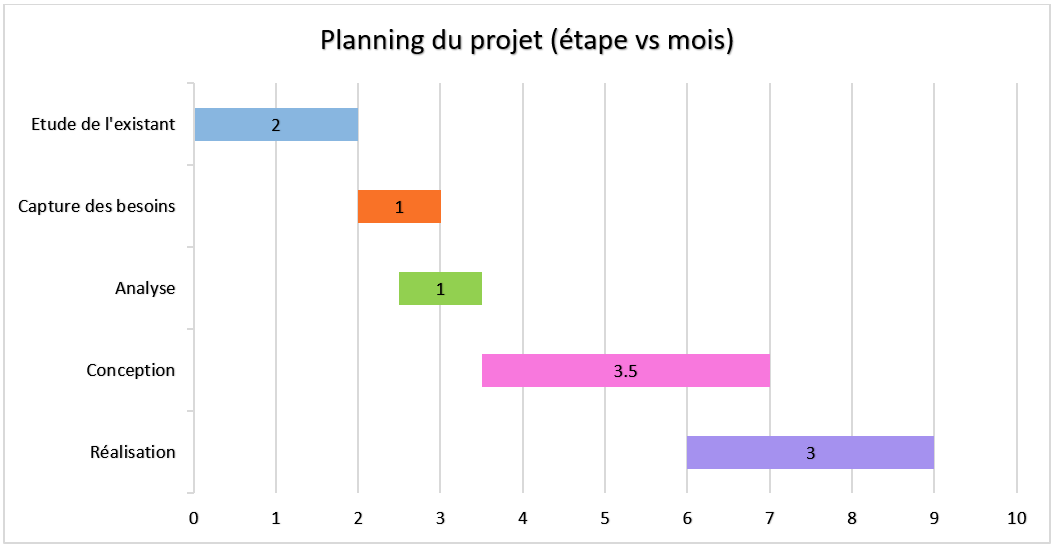
\includegraphics[width=0.9\linewidth]{./image_chapitre1/gant}
	\caption[Planning du projet]{Planning du projet}
	\label{fig:gant}
\end{figure}
\section{Organisation du m�moire}
Ce pr�sent document, qui repr�sente notre rapport de stage de fin d'�tude � SAIDAL, est
structur� en 4 grandes parties :
\subsubsection*{Partie 01: �tude bibliographique}
Nous commen�ons par une �tude bibliographique afin de d�finir et d'expliquer les concepts de
base.
\subsubsection*{Partie 02: �tude de l'existant}
Nous faisons ici une analyse de l'organisme d'accueil, ainsi que de la fonction maintenance.
L'objectif de cette analyse est de d�finir les probl�mes actuels afin
de parvenir � proposer la solution la plus ad�quate au contexte de la fonction maintenance de
SAIDAL.\\[0.5\baselineskip]
Cette �tude recouvre plusieurs axes : m�tier, applicatif, organisationnel.
\subsubsection*{Partie 03: La solution}
Dans cette partie nous pr�sentons la solution pr�conis�e pour la r�solution des diff�rents
probl�mes d�tect�es auparavant.
\subsubsection*{Partie 04: Conclusion et perspectives}
Pour finir, nous pr�sentons notre conclusion, ainsi que les perspectives.


\include{pagevide}
\chapter{\sc Synth�se bibliographique}\label{chap2}
Dans ce deuxi�me chapitre, nous introduisons, d'abord, quelques g�n�ralit�s sur la maintenance. Nous nous int�ressons principalement sur les types de maintenance ainsi que les op�rations associ�s � sa gestion. Par la suite, nous pr�senterons les concepts cl�s de la maintenance assist�es par ordinateur (GMAO). 
\section{Maintenance}
\subsection{D�finitions}
Nous allons pr�senter ici deux d�finitions de la maintenance.
\subsubsection{D�finition AFNOR X 60-010 (d�cembre 1994)}
Selon la norme NF X 60-010 donn�e par l'AFNOR (Association Fran�aise de Normalisation), la maintenance est d�finie comme �tant : � ensemble des actions permettant de maintenir ou de r�tablir un bien dans un �tat sp�cifi� ou en mesure d'assurer un service d�termin� �. \cite{ref01}\\[0.5\baselineskip]
Cette d�finition peut �tre compl�t�e par le document d'introduction � la maintenance X 60-000 qui pr�cise: �Bien maintenir, c'est assurer ces op�rations au co�t global optimal.�\cite{ref01}\\[0.5\baselineskip]
A partir de cette d�finition, nous pouvons tirer deux mots cl�s importants :
\begin{itemize}
	\item Action de maintenir: contient la notion de surveillance et de pr�vention sur un bien en fonctionnement normal. \cite{ref01}
	\item Action de pr�venir: contient la notion de correction (remise � niveau) apr�s perte de fonction. \cite{ref01}
\end{itemize}
\subsubsection{D�finition CEN projet WI 319-003 (1997)}
Selon le CEN (Comit� europ�en de normalisation), La maintenance est �l'ensemble de toutes les actions techniques, administratives et de
gestion durant le cycle de vie d'un bien, destin�e � le maintenir ou � le r�tablir dans
un �tat dans lequel il peut accomplir la fonction requise�.\cite{ref01}\\[0.5\baselineskip]
La fonction requise est ainsi d�finie : �fonction, ou ensemble de fonctions d'un bien
consid�r�es comme n�cessaire pour fournir un service donn�.\cite{ref01}\\[0.5\baselineskip]
L'op�ration de maintenance peut se d�finir comme �tant une suite d'actions organis�es, intervenant sur un syst�me et ayant deux objectif:
\begin{itemize}
	\item \textbf{Premier objectif: }r�tablir un bien, en �tat de dysfonctionnement et le replacer en �tat
	de fonctionnement, donc de produire.\cite{ref01}
	\item \textbf{Deuxi�me objectif: }maintenir ce bien, par une suite d'actions pr�ventives et planifi�es,
	en �tat parfait de fonctionnement, donc de produire. En r�gle g�n�rale, le service maintenance doit garder l'outil de production en �tat op�rationnel, afin d'assurer une production efficace et maximale.\cite{ref01}
\end{itemize}

%\subsubsection*{Diff�rence entre entretien et maintenance}
%\noindent \textbf{Entretien: }ce terme d�signe les op�rations ou les interventions � effectuer sur un
%mat�riel de production afin de le conserver en parfait �tat de produire. Les op�rations correspondantes, souvent ordonn�es par le constructeur, peuvent prendre la forme:
%\begin{itemize}
%	\item De vidange (huile de lubrification),
%	\item De graissage (paliers de guidage),
%	\item De changement de courroies, etc.\cite{r2}
%\end{itemize}

%\noindent \textbf{Maintenance: }la maintenance permet d'organiser, pr�voir, planifier et g�rer les
%op�rations d'entretien. La maintenance permet donc de conserver un bien dans son �tat maximal de %production. Aux activit�s techniques effectu�es par des sp�cialistes viennent se greffer d'autres %responsabilit�s comme:
%\begin{itemize}
%	\item l'organisation d'une structure de maintenance pr�ventive,
%	\item le suivi des co�ts,
%	\item l'analyse des pannes ainsi que le compte rendu des interventions de maintenance,
%	\item le suivi informatique du vieillissement du mat�riel,
%	\item l'�tablissement d'un fichier historique du suivi de maintenance par secteur et par machine,
%	\item la gestion des stocks de pi�ces d�tach�es.\cite{r2} 
%\end{itemize}
\subsection{Types de la maintenance}
Principalement, nous avons deux types de la maintenance : la maintenance pr�ventive qui est effectu�e avant l'arriv�e de la panne et la maintenance corrective qui est effectu�e apr�s l'arriv�e de la panne. Nous d�finissons dans la ci-dessous ces deux types de maintenance et leurs sous types.

\begin{figure}[H]
	\centering
	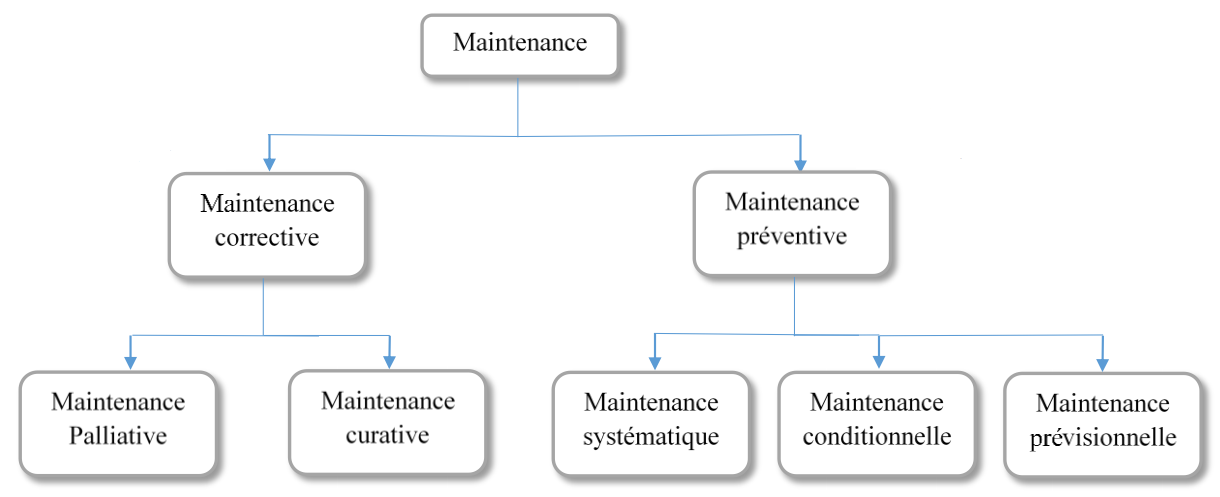
\includegraphics[width=0.9\linewidth]{./image_chapitre2/types}
	\caption[Les diff�rents types de maintenance]{Les diff�rents types de maintenance}
	\label{fig:types}
\end{figure}

\subsubsection{Maintenance pr�ventive}
La maintenance pr�ventive est une � maintenance ex�cut�e � des intervalles pr�d�termin�s ou selon des crit�res prescrits et destin�s � r�duire la probabilit� de d�faillance ou la d�gradation du fonctionnement d'un bien � \cite{ref02}. Elle est divis�e en :\\[0.5\baselineskip]
\noindent \textbf{Maintenance conditionnelle:}

La maintenance conditionnelle est une � maintenance pr�ventive bas�e sur une surveillance du fonctionnement du bien et/ou des param�tres significatifs de ce fonctionnement et int�grant les actions qui en d�coulent �. \cite{ref02}
\vspace{0.3cm}

\noindent \textbf{Maintenance pr�visionnelle}

La maintenance pr�visionnelle est une � maintenance conditionnelle ex�cut�e en suivant les pr�visions extrapol�es de l'analyse et de l'�valuation de param�tres significatifs de la d�gradation du bien �. \cite{ref02}
\vspace{0.3cm}

\noindent \textbf{Maintenance syst�matique}

La maintenance syst�matique est une � maintenance pr�ventive ex�cut�e � des intervalles de temps pr��tablis ou selon un nombre d�fini d'unit�s d'usage mais sans contr�le pr�alable de l'�tat du bien �. \cite{ref02}

\subsubsection{Maintenance corrective}
La maintenance corrective est une � maintenance ex�cut�e apr�s d�tection d'une panne et destin�e � remettre un bien dans un �tat dans lequel il peut accomplir une fonction requise � \cite{ref02}. Elle est subdivis�e en :\\[0.5\baselineskip]
\noindent \textbf{Maintenance palliative}

La maintenance palliative est une � Action de maintenance corrective destin�e � permettre � un bien d'accomplir provisoirement tout ou partie d'une fonction requise �. Elle est souvent appel�e � d�pannage � qui doit �tre suivi d'une maintenance curative. \cite{ref02}
\vspace{0.3cm}

\noindent \textbf{Maintenance curative}

La maintenance curative est une � Action de maintenance corrective ayant pour objet de r�tablir un bien dans un �tat sp�cifi� pour lui permettre d'accomplir une fonction requise �. Ce type de maintenance doit donner un caract�re permanent pour rem�dier � la panne. \cite{ref02}

\subsection{Niveaux de maintenance}
Les op�rations de la maintenance sont souvent nombreuses, parfois r�p�titives et parfois occasionnelles, d'o� la n�cessit� de la hi�rarchisation en niveaux \cite{ref02}. Selon la norme AFNOR X 60-000, il existe 5 niveaux de maintenance:

\begin{itemize}
\item \textbf{1er niveau:}

Op�rations  simples r�alis�es sur des �l�ments facilement accessibles en toute s�curit�.
Ce type d'actions peut �tre ex�cut�  par l'utilisateur du bien. \cite{ref02}\\[0.5\baselineskip]
\noindent Exemples:
\begin{itemize}
	\item Maintenance corrective: remplacement des lampes, ajustage d'�l�ments d�t�rior�s, etc ...
	\item Maintenance pr�ventive: test des lampes, graissage journaliers, etc ...
\end{itemize}
\item \textbf{2�me niveau:}

Actions simples d�finies dans les instructions de maintenance, qui sont ex�cut�es par un personnel qualifi� avec des proc�dures simples mais d�taill�es et des �quipements de soutien. \cite{ref02}\\[0.5\baselineskip]
\noindent Exemples:
\begin{itemize}
	\item Maintenance corrective: remplacement par �change standard de pi�ces (fusibles, courroies, filtres � air).	
	\item Maintenance pr�ventive: remplacement des filtres difficile d'acc�s.
\end{itemize}

\item \textbf{3�me niveau}

Actions qui n�cessitent des �quipements et des proc�dures complexes, ex�cut�es par un technicien qualifi�. \cite{ref02}\\[0.5\baselineskip]
\noindent Exemples:
\begin{itemize}
	\item Maintenance corrective: r�paration d'une fuite d'un fluide.	
	\item Maintenance pr�ventive: contr�le d'allumage de chaudi�res. 
\end{itemize}

\item \textbf{4�me niveau}

Op�rations dont des proc�dures complexes qui impliquent une ma�trise de technologie particuli�re et une mise en \oe uvre d'�quipements sp�cialis�s. \cite{ref02}\\[0.5\baselineskip]
\noindent Exemples:
\begin{itemize}
	\item Maintenance corrective: remplacement de clapets de compresseur.	
	\item Maintenance pr�ventive: analyse vibratoire, analyse des lubrifiants.	
\end{itemize}

\item \textbf{5�me niveau}

Op�rations dont les proc�dures impliquent un savoir-faire, des techniques, des technologies particuli�res et des �quipements de soutien industriels complexes. Ce type d'op�rations n�cessite l'intervention du constructeur ou une soci�t� sp�cialis�e. \cite{ref02}\\[0.5\baselineskip]
\noindent Exemples:
\begin{itemize}
	\item r�visions g�n�rales avec le d�montage complet de la machine.	
	\item reprise dimensionnelle et g�om�trique.	
\end{itemize}
\end{itemize}
\subsection{Objectifs de la maintenance}
\begin{itemize}

\item \textbf{Contribuer � assurer la production pr�vue (Quantit�):}

La planification de la production doit �tre �tudi�e parall�lement par la maintenance et la production en trouvant un consensus entre les arr�ts n�cessaires � la maintenance pr�ventive et les recommandations du service production et cela pour le but de produire la quantit� d�sir�e en tenant compte de la disponibilit� des �quipements. \cite{ref03}

\item \textbf{Contribuer � maintenir la qualit� du produit fabriqu� (Qualit�):}

La qualit� d�pend autant de la production que de la maintenance. Elle peut co�ter cher et c'est pourquoi il est indispensable de consid�rer les besoins de maintenance au m�me titre que les autres moyens de contr�le de la qualit�.\cite{ref03}
\item \textbf{Contribuer au respect des d�lais (d�lais):}

On parle ici autant des d�lais de fabrication des produits que des d�lais d'intervention en maintenance. Il y a donc une double responsabilit� au niveau de la maintenance : on doit conna�tre exactement l'�tat des �quipements pour en garantir leur fonctionnement pendant les p�riodes de production et on doit s'assurer de pr�parer et prioriser les travaux de maintenance avec suffisamment de pr�cision pour les r�aliser dans les d�lais avec un maximum d'efficacit�.\cite{ref03}
\item \textbf{Rechercher des co�ts optimaux (Rentabilit�):}

Mis � part les comp�tences techniques, le service de la maintenance doit �tre capable d'�tablir des devis estimatifs reli�s aux travaux de maintenance. Que ce soit pour chiffrer les diff�rentes solutions, pour proposer le remplacement d'une machine, pour soumettre un projet d'am�lioration ou de mise � niveau d'un �quipement.\cite{ref03}
\item \textbf{Respecter la s�curit� des travailleurs et la qualit� du milieu de travail (S�curit�):}

Le service de la maintenance doit se pr�occuper de la s�curit� des travailleurs lors des interventions qui peuvent toucher d'une part ses propres t�ches (m�thodes de travail, consignes de s�curit�, etc ...) et d'autre part, le personnel de production (remise des protecteurs, consid�rations pour la s�curit� lors de modifications d'�quipement, etc ...).\cite{ref03}
\item \textbf{Respecter l'environnement:}

Il est impos� au service de la maintenance de faire le contr�le de ses d�chets puisqu'ils peuvent �tre des polluants ou des contaminants de l'environnement.\cite{ref03}
\end{itemize}
\subsection{Documentation de la maintenance}
Une bonne connaissance du mat�riel passe par une documentation suffisamment
exhaustive pour prendre en compte tous les �quipements n�cessitant un suivi, une politique de
maintenance et un stockage de pi�ces de rechange. On dira m�me que la documentation est
un des piliers de la fonction maintenance et est indispensable � celle-ci afin qu'elle puisse
accomplir sa mission le mieux possible. \cite{web01}\\[0.5\baselineskip]
La fonction maintenance exige la circulation appropri�e des informations entre les diff�rents
n\oe uds de son organisation interne \cite{web01}. La documentation intervient donc � tous les niveaux du
service maintenance :
\begin{itemize}
	\item Dossiers techniques pour la pr�paration d'interventions plus efficaces et plus s�res.
	\item Modes op�ratoires pour les interventions proprement dites.
	\item Dossiers historiques pour la politique de maintenance � mettre en place.
	\item Catalogues constructeurs pour la gestion du stock maintenance.
\end{itemize}
La structure g�n�rale de la documentation d'un service maintenance est donn�e ci-dessous.
Cette documentation se d�compose en deux grandes parties : la documentation g�n�rale et la
documentation strat�gique.
\begin{figure}[H]
	\centering
	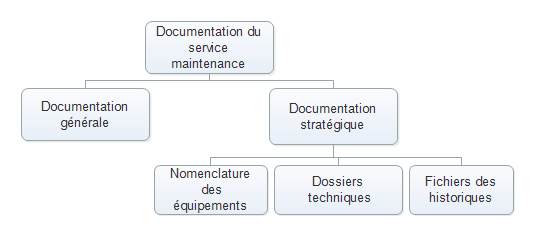
\includegraphics[width=0.8\linewidth]{./image_chapitre2/documentation}
	\caption[Structure de la documentation du service maintenance]{Structure de la documentation du service maintenance\cite{web01}}
	\label{fig:documentation}
\end{figure}
\subsubsection*{Documentation g�n�rale}
Le service se doit de se doter d'un service de documentation g�n�rale, mis � jour
r�guli�rement. Celle-ci comprend tous les documents techniques qui ne sont pas affect�s � des
mat�riels particuliers, mais qui sont n�cessaires aux maintenanciers pour r�pondre � des
questions techniques plus g�n�rales \cite{web01}. Elle contient en particulier :
\begin{itemize}
	\item tous les ouvrages de technique fondamentale (m�canique, �lectricit�, hydraulique,
	pneumatique, thermique) o� l'on trouvera les formulaires et abaques n�cessaires au
	dimensionnement rapide d'�l�ments techniques ou de composants. \cite{web01}
	\item des ouvrages plus sp�cialis�s, destin�s � des lecteurs plus avertis, et tr�s utiles lorsqu'on
	veut conduire une �tude d'am�lioration et de fiabilisation d'un �quipement. \cite{web01}
\end{itemize}
\subsubsection*{Documentation strat�gique}
Elle se d�compose en quatre grandes parties:
\begin{itemize}
	\item La nomenclature des �quipements.
	\item Le dossier technique des �quipements.
	\item Le fichier des historiques.
\end{itemize}
\begin{enumerate}
	\item \textbf{Nomenclature des �quipements:}\\[0.5\baselineskip]
	La nomenclature est une liste exhaustive qui comporte la d�signation des pi�ces qui rentrent
	dans la composition d'un �quipement. La d�composition est faite de fa�on arborescente de
	plusieurs niveaux, chaque n\oe ud (�quipement, organe ... pi�ce) est identifi� par un code
	(codification) \cite{ref06}. La nomenclature peut se faire sous forme de sch�mas.\\[0.5\baselineskip]
	Tous les mat�riels et biens durables de l'entreprise doivent �tre inventori�s, class�s et codifi�s
	afin de constituer une nomenclature. Une telle nomenclature va faciliter l'�tablissement des
	budgets de maintenance, la mise en place de plans de maintenance pr�ventive et plus
	g�n�ralement des m�thodes de maintenance. \cite{web01}
	\item \textbf{Dossier technique d'un �quipement:}\\[0.5\baselineskip]
	Le dossier technique comprend tous les renseignements et documents qui concernent un m�me
	type de mat�riel \cite{web01}:
	\begin{itemize}
	\item Les �l�ments d'identification : d�signation du type, constructeur, caract�ristiques g�n�rales,
	liste des machines du m�me type, fiche technique. \cite{web01}
	\item Le r�pertoire des documents class�s dans le dossier. \cite{web01}
	\item La synth�se des modifications effectu�es sur ces machines. \cite{web01}
	\end{itemize}
	Le dossier est consult� lors des interventions de maintenance, pr�paration d'intervention ou lors
	du d�pouillement d'une expertise.
	
	\item \textbf{Fichier historique de l'�quipement:}\\[0.5\baselineskip]
	C'est la partie de la documentation de maintenance qui enregistre les d�faillances,
	pannes et informations relatives � la maintenance d'un bien. Elle retrace la vie du mat�riel en
	indiquant chronologiquement tous les faits marquants de maintenance ainsi que les
	am�liorations qui auront �t� apport�es � l'�quipement depuis sa mise en service. \cite{web01}
\end{enumerate}

\subsection{La maintenance et les autres fonctions de l'entreprise}
L'organisation de la maintenance est justifi�e par le type de l'entreprise. Elle doit correspondre au champ d'activit�s et la sp�cialit� de cette derni�re.\\[0.5\baselineskip]
Pour les diff�rentes entreprises, l'urgence en cas de panne est tr�s importante pour les unes et moins pour les autres, les d�cisions � prendre seront donc tr�s diff�rentes. De plus, pour am�liorer la maintenance, il est impossible d'isoler cette fonction des autres fonctions de l'entreprise. Il faut donc int�grer et faire participer � son organisation d'autres fonctions qui ont plus ou moins une influence sur sa gestion et son organisation, donc sur ses co�ts et son efficacit�. Ces fonctions doivent avoir des objectifs communs ou concert�s avec la fonction maintenance. \cite{ref03}\\[0.5\baselineskip]
Ces fonctions sont:
\begin{itemize}
	\item \textbf{Achats:}
	
	Pour faire respecter le cahier des charges et les sp�cifications techniques de qualit� n�cessaires pour les �quipements achet�s aupr�s des fournisseurs, pour et pour obtenir le dossier technique le mieux adapt� aux politiques de la maintenance de l'entreprise. \cite{ref03}
	\item \textbf{Gestion des actifs:}
	
	Pour les programmes d'investissement, l'�tude des installations, les �tudes de fiabilit� et de maintenabilit�, la standardisation du mat�riel, la documentation technique des constructeurs, le choix des sous-traitants et des entrepreneurs, la r�ception technique du mat�riel sont � la charge de la gestion des actifs. \cite{ref03}
	\item \textbf{M�thodes de fabrication:}
	
	Le service m�thodes et fabrication donne au service maintenance les proc�dures d'utilisation des �quipements, leur taux d'utilisation, le niveau de s�curit� de ce mat�riel et du personnel de fabrication et la documentation technique des �quipements. \cite{ref03}
	\item \textbf{Gestion des stocks:}
	
	L'�tablissement du catalogue magasin de fournitures des pi�ces de rechange de la maintenance, leur m�thode de gestion, leur classement dans ce magasin, la r�duction de leur co�t de possession (quantit� minimale et maximale) sont confi�s au service de gestion des stocks. \cite{ref03}
	\item \textbf{Contr�le de la qualit� et la normalisation:}
	
	Le service qualit� a un r�le primordial dans l'entreprise et notamment dans la maintenance. Il est charg� d'effectuer des �tudes garantissant la qualit� de la maintenance, �laborer les plans d'action aupr�s du personnel charg� de la maintenance, assurer le suivi quotidien de la mise en \oe uvre de la politique de maintenance de l'entreprise et veiller � ce que la nomenclature des �quipements de la maintenance et la standardisation des composants et des installations r�pondent aux normes en vigueur. \cite{ref03}
	\item \textbf{Finances:}
	
	Le service Finances est charg� d'�tablir les relations �conomiques entre l'amortissement et la maintenance des �quipements, les cycles de r�visions �conomiques du mat�riel et la d�cision de remplacement quand le cycle devient trop couteux. \cite{ref03}
	\item \textbf{S�curit�:}
	
	Le service s�curit� est charg� de la s�curit� du personnel et du mat�riel pour am�liorer les conditions de travail en assurant un syst�me de maintenance s�curis� et efficace dans l'organisation du travail. \cite{ref03}
\end{itemize}
\begin{figure}[H]
	\centering
	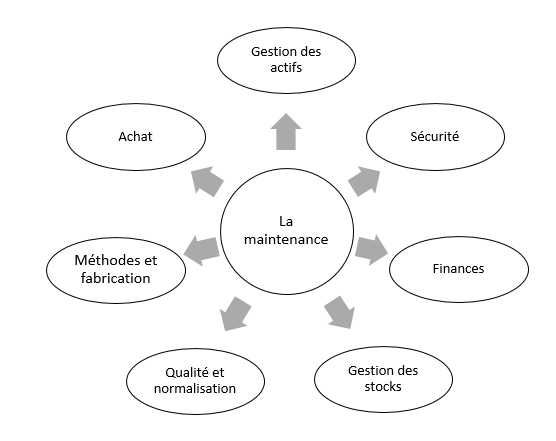
\includegraphics[width=0.6\linewidth]{./image_chapitre2/maintenanceetautres}
	\caption[La maintenance et les autres fonctions de l'entreprise]{La maintenance et les autres fonctions de l'entreprise}
	\label{fig:maintenanceetautres}
\end{figure}
\subsection{Pr�sentation d'un syst�me de gestion de la maintenance:}
La fugure ci-dessous que nous pr�sentons repr�sente le syst�me de gestion de la maintenance. Il comporte quatre �tapes:
\begin{itemize}
	\item La premi�re �tape concerne la r�ception du mat�riel.
	\item La deuxi�me est relative au choix du type de maintenance � appliquer en fonction des param�tres choisis.
	\item A partir du type de maintenance choisi (conditionnelle, syst�matique ou corrective), nous pr�cisons les �tapes du processus de maintenance telles que la planification des interventions, les proc�dures de d�tection des d�faillances, l'ex�cution et le suivi de l'intervention.
	\item La derni�re �tape concerne la r�alisation et le suivi de l'op�ration de maintenance.	
\end{itemize}
\newpage
\begin{figure}[H]
	\centering
	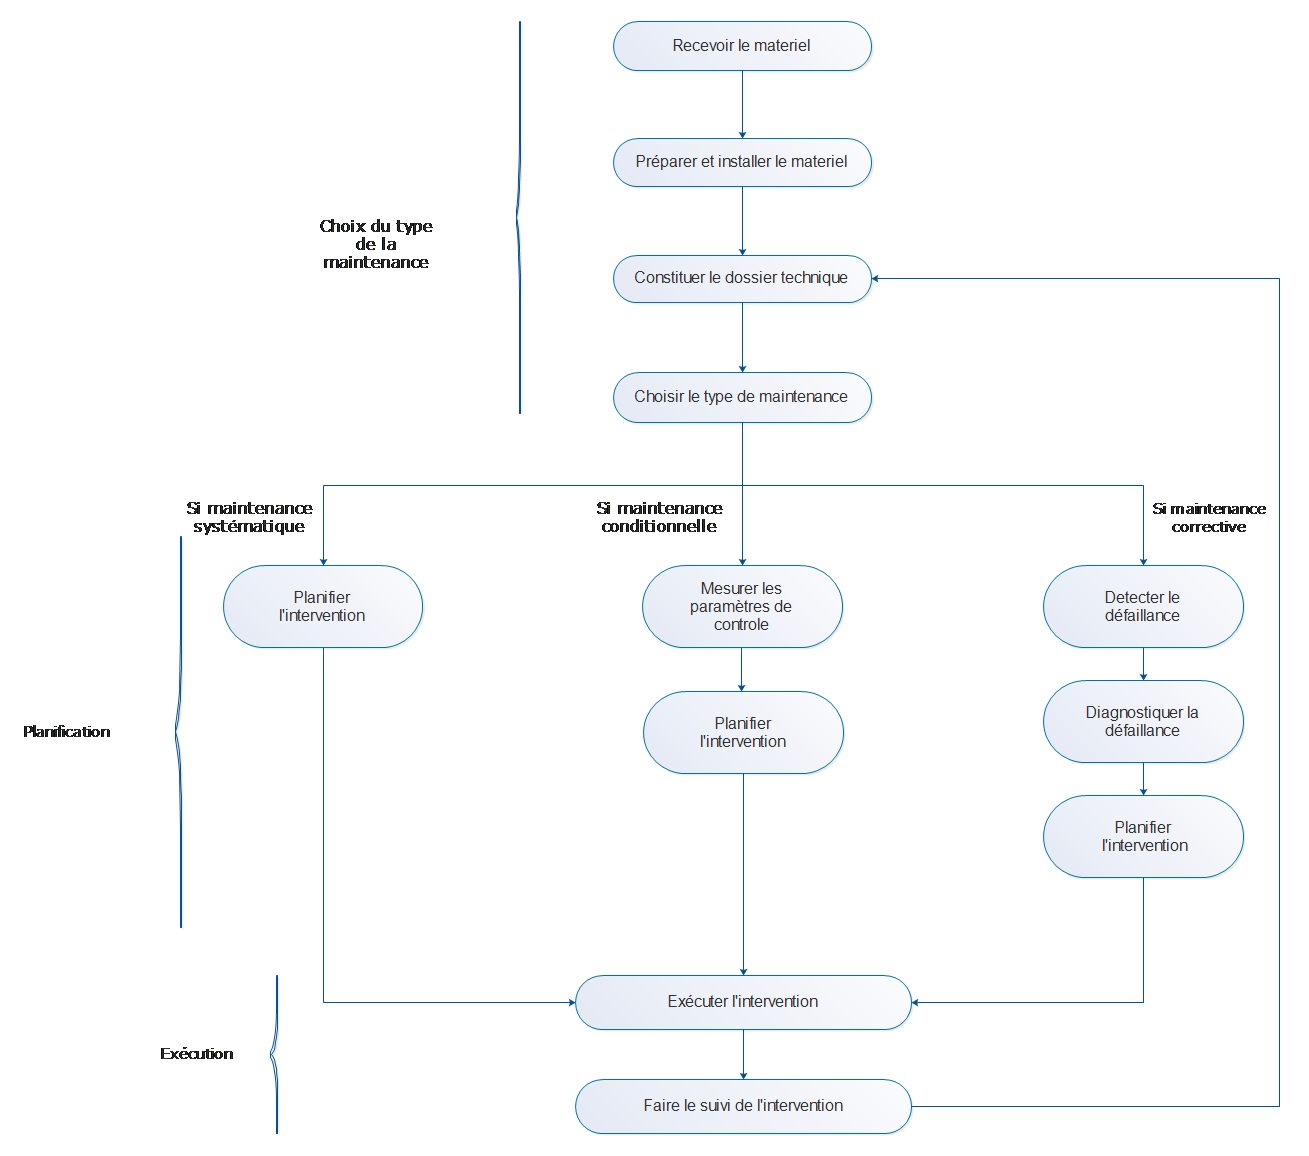
\includegraphics[width=1\linewidth]{./image_chapitre2/systeme}
	\caption[Le syst�me de gestion de maintenance]{Le syst�me de gestion de maintenance \cite{ref04}}
	\label{fig:syst�me}
\end{figure}



\section{Gestion de maintenance assist�e par ordinateur (GMAO)}
\subsection{D�finition de la GMAO}
\subsubsection*{D�finition 1}

En 1985, M.Gabriel et Y.PIMOR d�finissent la GMAO en ces termes:
� Un syst�me informatique de management de la maintenance est un progiciel organis� autour
d'une base de donn�es permettant de programmer et de suivre sous les trois aspects techniques,
budg�taire et organisationnel, toutes les activit�s d'un service de maintenance et les objets de
cette activit� (services, lignes d'atelier, machines, �quipements, sous-ensembles, pi�ces, etc.) �
partir de terminaux diss�min�s dans les bureaux techniques, les ateliers, les magasins et bureaux
d'approvisionnement.� \cite{web02}\\[0.5\baselineskip]
\subsubsection*{D�finition 2}

La GMAO ou Gestion de la Maintenance Assist�e par Ordinateur est un outil d'aide � la maintenance tr�s utilis� dans le monde industriel. La GMAO est utilis�e pour planifier des t�ches de maintenance, g�rer les fiches de suivi machines, les modes op�ratoires, les fiches d'intervention, indiquer aux op�rateurs les actions � effectuer, g�rer le stock de pi�ces de rechange, suivre l'historique des op�rations ... C'est un outil puissant mais qui demande � l'entreprise une politique de maintenance r�elle. \cite{ref05}

\subsection{Fonctionnalit�s d'un GMAO}
Les logiciels de GMAO ont progressivement int�gr� des fonctionnalit�s d�passant le cadre
des besoins d'un service de maintenance, en permettant une prise en charge plus globale
des processus associ�s aux �quipements. On va citer ici les principales fonctions d'un logiciel GMAO.
\begin{itemize}
	\item \textbf{Gestion des �quipements: }inventaire des �quipements, historique des travaux,
	gestion d'information d�di�e par type d'�quipement (b�timents, v�hicules, r�seaux, ordinateurs ...).
	\item \textbf{Gestion des actions de maintenance: } maintenance corrective (avec OT : ordre de travaux, ou BT : bon de travaux, ou ODM : ordre de maintenance), maintenance pr�ventive (syst�matique, conditionnelle, pr�visionnelle),gestion des outillages (utilis� pour r�aliser des actions de maintenance). Ce module inclut
	souvent des fonctionnalit�s ouvertes � des utilisateurs au-del� du service maintenance, comme une gestion des demandes d'intervention	(DI) permettant � toute personne autoris�e de l'entreprise de signaler une anomalie devant �tre prise en compte par le service de maintenance.
	\item \textbf{Gestion des stocks: }magasins (entr�s/sorties), quantit�s minimum et maximum de r�approvisionnement, r�f�rencement et recherche, articles de rechange, catalogue des fournisseurs, inventaire des pi�ces, ...
	\item \textbf{Gestion des achats :} demandes d'achat, commandes, bons de r�ception.
	\item \textbf{Gestion du pesonnel: }activit�s, m�tiers, planning de	charge, pr�visionnel, pointage des heures ...
	\item \textbf{Gestion des co�ts et budget: }de main d'\oe uvre, de stocks, d'achat, de	location de mat�riel, pr�paration des budgets, suivi p�riodique,...\cite{web03}
\end{itemize}

\subsection{Secteurs d'activit� concern�s par la GMAO}
Tous les secteurs d'activit� qui ont des �quipements � maintenir sont potentiellement concern�s par l'exploitation d'un outil de GMAO. On peut ainsi citer les secteurs:
\begin{itemize}
	\item de industrie (automobile, pharmaceutique, etc.),
	\item de l'�nergie (gaz, p�trole, �lectricit�, etc.),
	\item des transports (routier, ferroviaire, a�rien, transports publics, etc.),
	\item m�dicaux (h�pitaux, cliniques, etc.),
	\item des travaux publics,
	\item des t�l�coms (gestion des �quipements r�seau), ...
\end{itemize}

\subsection{Apport de la GMAO}
Aujourd'hui, dans nos entreprises modernes, la maintenance ne peut plus se r�sumer � des taches d'entretien basiques.
Il faut anticiper les pannes, afin de r�duire les co�ts et am�liorer la productivit�. En anticipant les pannes, on �vite des pannes machines trop longues et les co�ts de pertes de production li�s � ces pannes.
La GMAO s'av�re donc crucial pour l'am�lioration du service maintenance \cite{web04}. Donc l'avantage principal de la mise en place d'un GMAO est de faire basculer le ratio des interventions pr�ventives/correctives, en augmentant le nombre d'interventions pr�ventives au d�pend des correctives. Cependant, d'autres avantages existent, nous allons citer les les plus �vidents: 
\begin{itemize}
	\item L'information saisie est imm�diatement consultable sur le r�seau.
	\item Centralisation du stockage de l'information.
	\item D�centralisation de la consultation de l'information.
	\item Des documents claires, pr�cis et non discut�s.
	\item Conserver toutes les informations techniques d�finissant le mat�riel
	de production.
	\item Conserver et acc�der rapidement � tout l'historique des
	interventions.
	\item Organiser et faciliter le suivi des travaux pr�ventifs.
	\item Suivre le niveau des pi�ces en stock, conna�tre leurs
	caract�ristiques savoir sur quels �quipements elles sont install�es.
	\item Faciliter la gestion des achats de pi�ces et leur caract�ristiques techniques.
	\item Suivre les d�penses du service.
	\item Archiver et acc�der imm�diatement � toute la documentation
	technique maintenance.
	\item Meilleure organisation donc moins de stress, donc meilleure
	efficacit�. \cite{web04}
\end{itemize}

\subsection{March� des GMAO}
Selonune r�cente enqu�te de l'AFIM\footnote{Association fran�aise des ing�nieurs et responsables de maintenance}, il existerait pas moins de 800 logiciels de GMAO (et d'aides diverses � la maintenance) pour les applications industrielles \cite{web06}. Le site officiel de l'AFIM recense actuellement 69 progiciels et 59 �diteurs de logiciels GMAO et propose des comparatifs par fonction, prix, r�f�rences et chiffres d'affaires.\\[0.5\baselineskip]
En Alg�rie, il est plus difficile d'acc�der aux prix, par contre nous savons par exemple que les
�diteurs de logiciels leaders en Europe : Sage, et SAP sont implant�s en Alg�rie, et offrent des
suites ERP o� le module de GMAO peut �tre int�gr�. Le logiciel de GMAO OptiMaint est
largement connu aussi.\\[0.5\baselineskip]
Ci-dessous, nous allons pr�senter les principaux logiciels de GMAO qui existent actuellement sur le march�.

\begin{center}
	\begin{tabular}{|p{2cm}|p{1.8cm}|p{3.7cm}|p{3.7cm}|p{3.7cm}|}
		\hline
		\textbf{Nom} &  \textbf{Prix} & \textbf{Avantages} & \textbf{Ergonomie} & \textbf{Facilit� d'utilisation}    \\
		\hline
		\textbf{OPTIMa} & Environ 3300 \euro pour le monoposte et environ 500 \euro par License suppl�mentaires & Possibilit� de demander gratuitement un CD de d�monstration. Compatibilit� totale avec les logiciels de bureautique, complet : pas de modules suppl�mentaires � acqu�rir, multi-utilisateurs, avec diff�rents niveaux de droit, �volutif (personnalisable). Gestion technique, gestion des intervenants, gestion des pi�ces, gestion des travaux, analyse , fonctions diverses & Tr�s bonne � en croire le site car pas de visualisation disponible en ligne & Le param�trage est simplifi� et r�alis� lors de la premi�re utilisation. Vous n'avez pas besoin de plusieurs mois de travail avant d'�tre op�rationnel : OPTIMa est utilisable imm�diatement  \\
		\hline		
		\textbf{OptiMaint} & A partir de 2900 \euro & T�l�chargement gratuit de la version d�monstration en ligne. 
		Gestion du patrimoine, des interventions, des achats, des stocks, du budjet, de projets etc ... & Il s'interface avec les logiciels de GPAO, comptabilit�, gestion commerciale, achats, ERP, supervision ... , et permet les �changes d'informations entre logiciels afin d'�viter des doubles saisies inutiles et sources d'erreurs & Simple � mettre en place et imm�diatement op�rationnel, il alli une grande richesse fonctionnelle avec une facilit� d'utilisation. Cependant une formation des employ�s est propos�e  \\				
		\hline
	\end{tabular} \\
\end{center}
\newpage
\begin{center}
	\begin{tabular}{|p{2cm}|p{1.8cm}|p{3.7cm}|p{3.7cm}|p{3.7cm}|}
		\hline
		\textbf{Nom} &  \textbf{Prix} & \textbf{Avantages} & \textbf{Ergonomie} & \textbf{Facilit� d'utilisation}    \\
		\hline	
		\textbf{Q.I informatique} & Gratuit & Tout le logiciel est en t�l�chargement direct sur le site, avec des explications utiles et d�taill�es notamment une d�monstration & L'ergonomie est visible en t�l�chargeant les explications dans la rubrique "Fonctionnalit�s", celle ci � l'air correcte & Tr�s facile � prendre car tout est explicit� tr�s clairement par des d�monstrations \\
		\hline	
		\textbf{Altair} & A partir de 5000 \euro en fonction du nombre d'utilisateurs & Logiciel GMAO qui est en totalit� Web & Tr�s bonne ergonomie, tr�s complet. Il suffit de regarder les aper�us d'�crans sur le site de la firme & Enti�rement penser pour que l'utilisateur ne s'y perde pas \\
		\hline
	\end{tabular} \\
	\captionof{table}{Tableau comparatif des logiciels de GMAO \cite{web05}}
	\label{tab}
\end{center}
\begin{figure}[H]
	\centering
	
\includegraphics[width=1\linewidth]{./image_chapitre2/logos}
	\caption[logos des GMAO (Altair,OPTIMa, OptiMaint, Q.I informatique)]{logos des GMAO (Altair,OPTIMa, OptiMaint, Q.I informatique)}
	\label{fig:logos}
\end{figure}
\include{pagevide}

\chapter{\sc �tude de l'existant}
L'�tude de l'existant est une �tape primordiale dans la mise en place d'un syst�me
d'information. Elle permet de comprendre d'une part la structure de l'organisme d'accueil, son m�tier, ses objectifs ainsi que ses missions. Comme elle permet d'une autre part de d�cortiquer le fonctionnement du syst�me existant afin d'identifier les anomalies et d'en apporter des solutions.\\[0.5\baselineskip]
Ainsi, ce troisi�me chapitre est structur� comme suit:
\begin{itemize}
	\item Une bref pr�sentation de l'organisme d'accueil dans laquelle ce stage est effectu�,� savoir le groupe SAIDAL.
	\item une �tude d�taill�e du processus m�tier.
	\item Enfin,le diagnostic du syst�me existant.
\end{itemize}
\section{Pr�sentation du groupe SAIDAL}
 Le groupe industriel Sa�dal est une soci�t� par action (SPA) au capital social de
 \begin{wrapfigure}[4]{r}{3cm}
 	
\includegraphics[width=0.8\linewidth]{./image_chapitre3/Logo_SAIDAL}
    %\caption[Logo du groupe SAIDAL]{Logo du groupe SAIDAL}
 \end{wrapfigure}
 2.500.000.000 dinars alg�riens dont la mission principale est de d�velopper, produire et commercialiser les produits pharmaceutiques � usage humain et v�t�rinaire. Le groupe Sa�dal est consid�r� actuellement comme le leader de l'industrie pharmaceutique en Alg�rie avec une grande part de march�.
% \begin{figure}[H]
 %	\centering
 %	
\includegraphics[width=0.2\linewidth]{./image_chapitre3/Logo_SAIDAL}
 %	\caption[Logo du groupe SAIDAL]{Logo du groupe SAIDAL}
 %	\label{fig:saidal}
% \end{figure}
\subsection{Historique}
SAIDAL a �t� cr��e en avril 1982 � la suite de la restructuration de la Pharmacie Centrale Alg�rienne (PCA) et a b�n�fici�, dans ce cadre, du transfert des usines d'El Harrach, de Dar El Beida et de Gu� de Constantine. Il lui a �t� �galement transf�r� en 1988, le Complexe 'Antibiotiques' de M�d�a dont la r�alisation venait d'�tre achev�e par la SNIC (Soci�t� Nationale des Industries Chimiques).\\[0.5\baselineskip]
En 1989 et suite � la mise en \oe uvre des r�formes �conomiques, SAIDAL devint une entreprise publique �conomique dot�e de l'autonomie de gestion.\\[0.5\baselineskip]
En 1993, des changements ont �t� apport�s aux statuts de l'entreprise, lui permettant de participer � toute op�ration industrielle ou commerciale pouvant se rattacher � l'objet social par voie de cr�ation de soci�t�s nouvelles ou de filiales.\\[0.5\baselineskip]
En 1997, la soci�t� SAIDAL a mis en \oe uvre un plan de restructuration qui s'est traduit par sa transformation en groupe industriel regroupant trois filiales (Pharmal, Antibiotical et Biotic).\\[0.5\baselineskip]
En 2009, SAIDAL a augment� sa part dans le capital de SOMEDIAL � hauteur de 59\%. En 2010, elle a acquis 20 \% du capital d'IBERAL et sa part dans le capital de TAPHCO est pass�e de 38,75\% � 44,51\%.\\[0.5\baselineskip]
En 2011, SAIDAL a augment� sa part dans le capital d'IBERAL � hauteur de 60\%.\\[0.5\baselineskip]
En janvier 2014, Saidal a proc�d� par voie d'absorption, � la fusion de ses filiales d�tenues � 100\% :   Pharmal, Antibiotical et Biotic.\cite{web10}
\subsection{Missions}
En tant que premier producteur de m�dicaments g�n�riques en Alg�rie,  la mission premi�re de SAIDAL c'est:
\begin{itemize}
	\item De contribuer � la protection de  la sant� des citoyens et  � l'am�lioration de la qualit� des soins par la mise � disposition des patients, d'une gamme riche et diversifi�e de produits de qualit�,
	\item De prot�ger le droit des citoyens d'acc�der aux traitements par l'adoption d'une politique tarifaire favorisant de  larges couches de la soci�t�.
\end{itemize}
Sa position d'entreprise publique lui conf�re �galement la mission  d'accompagner la politique de sant� publique dans le d�veloppement de l'industrie pharmaceutique par le choix d'investissements orient�s vers la satisfaction des besoins  de la  population.\cite{web10}

\subsection{Organigramme g�n�rale du Groupe SAIDAL}
Le Groupe SAIDAL  a proc�d�  en janvier 2014 � la fusion,  par voie d'absorption, des  filiales ANTIBIOTICAL, PHARMAL et BIOTIC. Cette d�cision approuv�e  par ses organes sociaux a donn� lieu � une nouvelle organisation s'articulant autour de:
\begin{itemize}
	\item Une direction g�n�rale.
	\item Neuf (09) sites de production.
	\item Trois centres de distribution.
\end{itemize}
Cette structure organisationnelle est d�taill�e par l'organigramme suivant:
\begin{figure}[H]
	\centering
	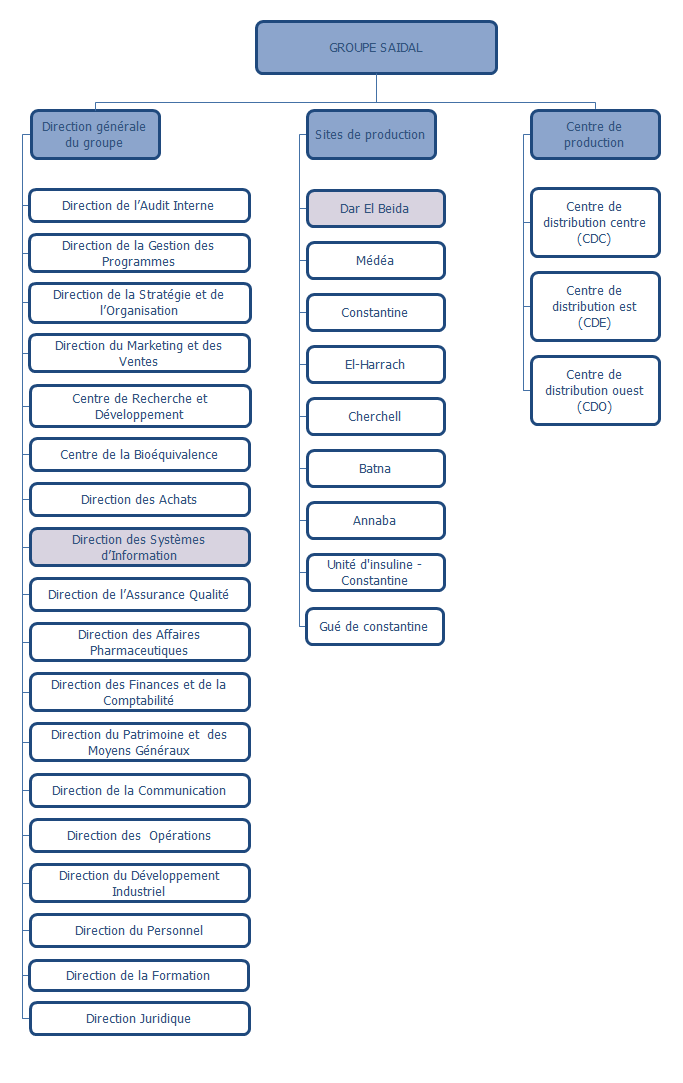
\includegraphics[width=0.8\linewidth]{./image_chapitre3/organigramme}
	\caption[Organigramme g�n�rale du Groupe SAIDAL]{Organigramme g�n�rale du Groupe SAIDAL}
	\label{fig:organigrammesaidal}
\end{figure}
\subsection{Site de production Dar El Beida}
C'est le site dans lequelle nous effectuerons notre stage. Il existe depuis 1958, il appartenait au laboratoire fran�ais LABAZ avant sa nationalisation en 1970, ce qui a donn� lieu aux transformations
suivantes:
\begin{itemize}
	\item Agrandissement du site de 3600 m2 � 6600 m2.
	\item La mise au point des produits pharmaceutiques alg�riens.
	\item Extension du magasin de stockage.
	\item Modernisation des cha�nes et des ateliers.
\end{itemize}
L'activit� de ce site �tait limit�e en la fabrication de quelques m�dicaments et produits
cosm�tiques, mais actuellement elle produit une gamme de m�dicaments tr�s large dans
plusieurs formes gal�niques (comprim�s, g�lules, sirops, forme p�teuses, suspension buvable, sels et solution dermique).\\[0.5\baselineskip]
Le site de production de Dar El Beida est caract�ris� par une capacit� de production tr�s
importante (43 millions unit�s de vente par an). Aussi l'usine est dot� d'un laboratoire de
contr�le de la qualit� charg� de l'analyse Physico-chimique et microbiologique et d'une
surface de stockage de 6600 m2 (4600 palettes).\cite{web10}
\subsection{Lieu d'affectation du stage: la sous-direction de maintenance}
Notre �tude s'effectuera au sein de la sous-direction de maintenance, qui est rattach� hi�rarchiquement � la direction de l'usine, charg� du suivi et de l'entretien des �quipements des ateliers de production.
L'organigramme suivant pr�sente la structure organisationnelle de la sous-direction de maintenance:
\begin{figure}[H]
	\centering
	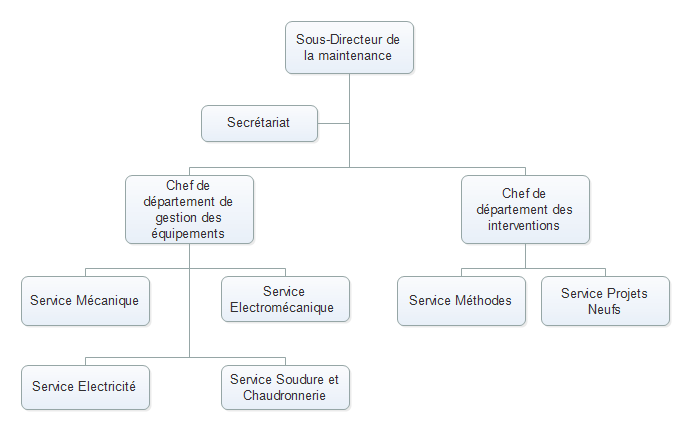
\includegraphics[width=.85\linewidth]{./image_chapitre3/organigramme_maintenance}
	\caption[organigramme du service de la maintenance]{organigramme du service de la maintenance}
	\label{fig:organigrammemaintenance}
\end{figure}
Chaque service est d�compos� comme suit :
\begin{figure}[H]
	\centering
	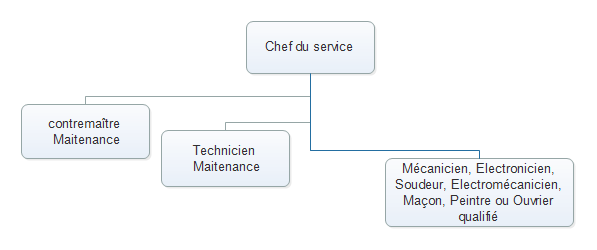
\includegraphics[width=0.8\linewidth]{./image_chapitre3/organigramme_maintenance_2}
	\caption[d�composition d'un service]{d�composition d'un service}
	\label{fig:organigrammemaintenance2}
\end{figure}
\section{Analyse de l'existant}
\subsection{�tude des postes de travail}
En organisation, un poste de travail est une unit� dans laquelle une personne ex�cute un ensemble de t�ches qui lui sont assign�es gr�ce aux ressources n�cessaires qui sont mises � sa disposition.
Notre �tude des postes de travail, a �t� faite gr�ce � l'analyse des fiches de poste qui nous sont fournies.\\[0.5\baselineskip]
Nous allons d�tailler les t�ches relatives aux diff�rents postes de travail. Notons que pour les niveaux 3 de la hi�rarchie, � savoir les chefs de service (voir figure 3.2 et figure 3.3), les t�ches sont tr�s semblables, donc nous avons d�cid� de restreindre l'�tude � un seul service dans chaque d�partement. Ainsi, les postes qui seront pr�sent�s sont:
\begin{itemize}
	\item Sous-directeur de la maintenance.
	\item Secr�taire.
	\item Chef de d�partement gestion des �quipements.
	\item Chef de d�partement des interventions.
	\item Chef de service m�canique.
	\item Contrema�tre en maintenance.
	\item Charg� des m�thodes.
	\item Technicien en maintenance.
\end{itemize}
\newpage

\subsubsection*{Fiche descriptive du poste N� 01}
\begin{center}
	\begin{tabular}{|p{2.7cm}|p{11.8cm}|}
		\hline	
		\textbf{Intitul� du poste} & Sous-directeur de la maintenance \\
		\hline	
		\textbf{Description des t�ches} & 
		\begin{itemize}
			\item Superviser l'entretien et le planning des �quipements et participe � la conception des nouvelles installations.
			\item Fixer les priorit�s et �laborer le planning de maintenance.
			\item �tablir, organiser et suivre le plan de maintenance pr�ventive.
			\item Manager les �quipes d'intervention et diriger les travaux d'intervention.
			\item G�rer les pi�ces de rechange.
			\item Pr�voir les comp�tences disponibles pour faire face aux al�as de fonctionnement.
			\item Identifier le solutions techniques d'am�lioration des �quipements et installations.
			\item G�rer la sous-traitance.
			\item G�rer le budget du service et pr�voir les investissements.
			\item Participer aux actions de qualit�, � la conception des nouvelles installations et le d�veloppement des nouveaux produits.
			%\item Pr�coniser la PDR n�cessaire au stock pour assurer un fonctionnement correct de l'outil de %production utilis�.
			\item D�terminer les besoins en formation de son personnel.
			%\item Veiller � l'application des BPF.
			\item Veiller au respect des consignes de s�curit� et d'hygi�ne.			
		\end{itemize}\\
		\hline
		 
	\end{tabular} \\
	\captionof{table}{Description du poste de travail � Sous-directeur de la maintenance �}
	\label{tab1}
\end{center}
\subsubsection*{Fiche descriptive du poste N� 02}
\begin{center}
	\begin{tabular}{|p{2.7cm}|p{11.8cm}|}
		\hline	
		\textbf{Intitul� du poste} & Secr�taire \\
		\hline	
		\textbf{Description des t�ches} & 
		\begin{itemize}
			\item Faire la saisie sur micro des diff�rents documents.
			\item Assurer l'enregistrement du courrier sur le registre (d�part et arriv�e).
			\item Assurer le classement des pi�ces administratives dans des chronos et dans dossiers personnels.
			\item Diffuser les diff�rentes correspondances.			
		\end{itemize}\\
		\hline
		
	\end{tabular} \\
	\captionof{table}{Description du poste de travail � Secr�taire �}
	\label{tab2}
\end{center}

\subsubsection*{Fiche descriptive du poste N� 03}
\begin{center}
	\begin{tabular}{|p{2.7cm}|p{11.8cm}|}
		\hline	
		\textbf{Intitul� du poste} & Chef de d�partement de gestion des �quipements \\
		\hline	
		\textbf{Description des t�ches} & 
		\begin{itemize}
		    \item Suivre l'activit� des diff�rents services au quotidien.
			\item Veiller � la codification des �quipements.
			\item Veiller � la tenue � jour des dossiers techniques et historiques des �quipements.
			\item D�terminer l'urgence des travaux.
			\item Programmer les travaux selon les urgences.
			\item Consulter et approuver les rapports d'activit�s mensuels.
			\item Participer � l'�laboration des plannings de maintenance pr�ventive et travaux neufs.
			\item Suivre le mouvement des �quipements avec le service patrimoine pour renforcer en collaboration avec la hi�rarchie et la production.			
			\item Veiller � l'application des consignes de s�curit� et BPF.
			\item Collaborer avec les gestionnaires des stocks pour l'achat des pi�ces de rechange.
			\item Participer � la faisabilit� et au d�veloppement des nouveaux produits sur les �quipements.
			\item Encadrer les apprentis et les stagiaires.		
		\end{itemize}\\
		\hline		
	\end{tabular} \\
	\captionof{table}{Description du poste de travail � Chef de d�partement de gestion des �quipements �}
	\label{tab3}
\end{center}
\subsubsection*{Fiche descriptive du poste N� 04}
\begin{center}
	\begin{tabular}{|p{2.7cm}|p{11.8cm}|}
		\hline	
		\textbf{Intitul� du poste} & Chef de d�partement des interventions \\
		\hline	
		\textbf{Description des t�ches} & 
		\begin{itemize}
			\item Assurer le bon fonctionnement des installations.
			\item Orienter et assister les subordonn�s lors des diff�rentes interventions.
			\item R�ceptionner et traiter les demandes de r�paration �tablies par les diff�rents services.
			\item Proc�der au diagnostic des pannes.
			
		\end{itemize}\\
		\hline
\end{tabular} \\
\end{center}			
\newpage	
\begin{center}
	\begin{tabular}{|p{2.7cm}|p{11.8cm}|}
		\hline		
		\textbf{Description des t�ches} &	
		\begin{itemize}
			\item Attribuer les t�ches aux subordonn�s.
			\item Proc�der � la r�paration �lectrique et m�canique des machines et installations.
			\item Proc�der � la maintenance pr�ventive et curative des �quipements de production utilis�s.
			\item Participer � l'�tude technique des offres des �quipements.
			\item Collaborer avec le bureau des m�thodes � l'�laboration des plannings d'interventions et travaux neufs.	
			\item Pr�coniser et r�ceptionner avec le bureau des m�thodes, les travaux de soudure et installations.
			\item Proc�der � l'installation �lectrique, industrielle et b�timents.
			\item Assurer la maintenance des chariots �l�vateurs �lectriques.
			\item Assister et suivre la sous-traitance.
			\item Faire appliquer les consignes de s�curit�.
			\item Appliquer et tester les exigences des BPF.		
		\end{itemize}\\
		\hline		
	\end{tabular} \\
	\captionof{table}{Description du poste de travail � Chef d�partement des interventions �}
	\label{tab4}
\end{center}
\subsubsection*{Fiche descriptive du poste N� 05}
\begin{center}
	\begin{tabular}{|p{2.7cm}|p{11.8cm}|}
		\hline	
		\textbf{Intitul� du poste} & Chef de service m�canique \\
		\hline
		\textbf{Description des t�ches} & 
		\begin{itemize}
			\item Contr�ler les absences de ses subordonn�s.
			\item Contr�ler l'�tat de fonctionnement des machines.
			\item Distribuer les t�ches aux subordonn�s.
			\item R�ceptionner les demandes de r�paration �tablies par les services de production.
			\item Proc�der � la r�paration m�canique des machines, compresseurs, chariots, �l�vateurs et transpalettes.
			\item Proc�der au diagnostics des pannes.
			\item Proc�der au changement de format des machines de fabrication ou de conditionnement.
			\item Contr�ler et remplacer les pi�ces d'usure des machines.		
		\end{itemize}\\
		\hline		
	\end{tabular} \\
	\captionof{table}{Description du poste de travail � Chef de service m�canique �}
	\label{tab5}
\end{center}
\newpage
\subsubsection*{Fiche descriptive du poste N� 06}
\begin{center}
	\begin{tabular}{|p{2.7cm}|p{11.8cm}|}
		\hline	
		\textbf{Intitul� du poste} & contrema�tre en maintenance \\
		\hline	
		\textbf{Description des t�ches} & 
		\begin{itemize}
			\item Contr�ler l'�tat de fonctionnement des machines.
			\item R�ceptionner les demandes de r�paration �tablies par les diff�rents services.
			\item Proc�der � la r�paration des machines.
			\item Participer aux diagnostics des pannes.
			\item Participer au changement de format des machines de fabrication ou de conditionnement.
			\item Participer � la r�ception des nouveaux �quipements et des installations.
			\item Appliquer les normes de BPF.
			\item Encadrer ses �l�ments.
			\item Veiller � l'application des consignes de s�curit�.
			\item L'entretien de son outillage.						
		\end{itemize}\\
		\hline		
	\end{tabular} \\
	\captionof{table}{Description du poste de travail � contrema�tre en maintenance �}
	\label{tab6}
\end{center}
\subsubsection*{Fiche descriptive du poste N� 07}
\begin{center}
	\begin{tabular}{|p{2.7cm}|p{11.8cm}|}
		\hline	
		\textbf{Intitul� du poste} & Charg� des m�thodes \\
		\hline	
		\textbf{Description des t�ches} & 
		\begin{itemize}
			\item Recevoir la demande de r�paration.
			\item D�terminer l'urgence avec le responsable concern�.
			\item Participer aux diagnostics des pannes.			
			\item �tablir, renseigner et transmettre l'ordre de service.
			\item Tenir � jour la saisie des rapports d'activit�s.
			\item Tenir � jour les dossiers historiques et techniques.
			\item Tenir � jour la documentation et renseigner le registre ad�quat.
			\item Suivre la sous-traitance et �tablir les PV de r�ception des travaux.			
		\end{itemize}\\
		\hline		
	\end{tabular} \\
	\captionof{table}{Description du poste de travail � Charg� des m�thodes �}
	\label{tab7}
\end{center}
\newpage
\subsubsection*{Fiche descriptive du poste N� 08}
\begin{center}
	\begin{tabular}{|p{2.7cm}|p{11.8cm}|}
		\hline	
		\textbf{Intitul� du poste} & Technicien en maintenance  \\
		\hline
		\textbf{Description des t�ches} & 
		\begin{itemize}
			\item Recevoir les demandes de r�paration.
			\item Diagnostiquer les pannes �lectriques, m�caniques, �lectrom�caniques ou celles relatives � la soudure en proc�dant � une s�rie de tests et de mesures.
			\item Suivre la sous-traitance et �tablir le PV des travaux.
			\item Tenir � jour la saisie des rapports d'activit�s.
			\item Tenir � jour les dossiers techniques et historiques.
			\item Renseigner les ordres de travail.
			\item Participer � l'installation et la d�sinstallation des nouveaux �quipements et ceux � d�placer.
			\item Participer � la pr�conisation des pi�ces de rechange.
			\item Participer � l'�laboration des plannings pr�ventifs des �quipements.
			\item Informer le bureau des m�thodes en cas de dysfonctionnement sur les �quipements.
			\item Veiller au respect des consignes de s�curit� et des BPF.				
		\end{itemize}\\
		\hline		
	\end{tabular} \\
	\captionof{table}{Description du poste de travail � Technicien en maintenance �}
	\label{tab8}
\end{center}
\subsubsection*{Synth�se}
Durant notre �tude des postes de travail, nous avons remarqu� quelques anomalies d'ordre organisationnel et humain, et qui sont : 
\begin{itemize}
\item Pr�sence de postes vacants dans l'organigramme, ce qui a entrain� des responsabilit�s qui ne sont pas assum�es.
\item Absence de quelques de fiches de postes.
\item Les missions ne sont pas convenablement r�alis�es et cela est d� peut-�tre au nombre important des missions pour chaque poste de travail.
\end{itemize}
\newpage
\subsection{�tude des documents}
Cette �tude nous permet de recenser les documents manipul�s par les postes de travail dans les diff�rentes proc�dures dans le service de maintenance du groupe industriel SAIDAL.

Dans le tableau ci-dessous, nous allons pr�senter pour chaque document:
\begin{itemize}
	\item Sa d�signation.
	\item Sa description.
	\item Son type (support), qui peut �tre:
	\begin{itemize}
		\item Papier.
		\item Num�rique.
	\end{itemize}
\end{itemize}
Voici la liste des documents que nous allons pr�senter dans cette �tude:
\begin{itemize}
	\item Dossier technique.
	\item Dossier historique.
	\item Demande de r�paration.
	\item Demande d'achat.
	\item Planning pr�ventif des �quipements.
	\item Bon de sortie des pi�ces.
	\item �tat des arr�ts journaliers.
	\item Rapport d'activit�s mensuel.
	\item Nomenclature de la documentation. 	
\end{itemize}
\begin{center}
	\begin{tabular}{|p{3cm}|p{9cm}|p{2cm}|}
		\hline
		\textbf{D�signation} & \textbf{Description} & \textbf{Type}  \\  
		\hline
		Dossier technique & Il est destin� � faciliter la mise en service et la mise en place du mat�riel. Il contient principalement les caract�ristiques techniques, les plans de d�limitation, la nomenclature des organes et les renseignements relatifs au constructeur et au fournisseur de l'�quipement. & papier  \\ 
		\hline 
		Dossier historique & Il contient toutes les �tapes d'o� passe le mat�riel : l'�tude, la commande, les informations concernant le fournisseur et le constructeur, la r�ception, l'essai et la mise en service. Il contient aussi les interventions et les modifications les plus importantes que subit l'�quipement. & papier \\
		\hline	
		Demande de r�paration & Il repr�sente une demande de service d'une fa�on formelle afin de  signaler une anomalie survenue sur un �quipement. & papier \\
		\hline
	\end{tabular} \\
\end{center}

\begin{center}
	\begin{tabular}{|p{3cm}|p{9cm}|p{2cm}|}
		\hline
		\textbf{D�signation} & \textbf{Description} & \textbf{Type}  \\  
		\hline
		Demande d'achat & C'est une demande effectu� � la direction des moyen g�n�raux  pour l'acquisition d'un �quipement ou une pi�ce de rechange & papier \\
		\hline	
		Planning pr�ventif des �quipements & C'est un calendrier des op�rations de la maintenance pr�ventive � ex�cuter chaque mois. & papier \\
		\hline
		Bon de sortie des pi�ces & Permet de justifier toute sortie d'une pi�ce de rechange du magasin. & papier \\
		\hline
		Etat des arr�ts journaliers & Contient tous les d�tails des interventions effectu�es chaque jour. & papier \\
		\hline
		Rapport d'activit� mensuel & R�sume l'ensemble des op�rations de maintenance effectu�es durant chaque mois en sp�cifiant le nombre et la dur�e des interventions,  la dur�e d'arr�t des �quipements ainsi que le co�t de chaque intervention. & Papier / num�rique \\
		\hline
		Nomenclature de la documentation & Liste la documentation technique livr�e avec chaque �quipement (manuel d'utilisation, Notice d'instruction, manuel d'installation, mode d'emploie , etc ...) & Papier \\
		\hline
	\end{tabular} \\
	\captionof{table}{Description des documents de la maintenance}
	\label{tab16}
\end{center}
\subsubsection*{Synth�se}
Durant notre �tude des documents, nous avons constat� quelques remarques et voici quelques-unes que nous jugeons importantes:
\begin{itemize}
	\item Tous les documents sont sur des supports papiers, ce qui qui peut engendrer leurs d�t�riorations.
	\item Les documents sont remplis manuellement, ce qui implique une perte de temps.
	\item La redondance des informations. Par exemple, le dossier technique et le dossier historique contiennent les m�mes renseignements concernant les fournisseurs et les constructeurs.
\end{itemize}
\subsection{�tude des proc�dures de travail}
Une proc�dure est un ensemble de t�ches qui concourent vers l'aboutissement d'un r�sultat pr�d�fini. L'�tude des proc�dures est une �tape importante dans la mise en place d'un syst�me d'information. En effet, elle permet de comprendre le fonctionnement du syst�me existant en d�cortiquant les enchainements des activit�s effectu�es et ensuite d�tecter les anomalies li�es � la gestion de la maintenance.\\[0.5\baselineskip]
Les informations contenues dans ces pr�sentes proc�dures ont �t� extraites des documents de la sous-direction de maintenance du groupe SAIDAL (Site de production DAR EL BAIDA), et lors de nombreuses interviews avec le responsable du service m�thode.\\[0.5\baselineskip]
Dans la suite, nous allons d�tailler les proc�dures de travail qui sont en nombre de sept (7) par une description textuelle puis par un sch�ma d�taill� (pour les proc�dures complexes). Pour le choix du formalisme � utiliser pour mod�liser ces proc�dures, nous avons opt� pour le diagramme d'activit�.\\[0.5\baselineskip]
Les proc�dures recens�es sont les suivantes:
\begin{itemize}
	\item Gestion de la documentation.
	\item R�ception et installation des �quipements.
	\item D�clenchements et r�ception des travaux de sous-traitance.
	\item Ordonnancement et r�alisation de la maintenance curative.
	\item Planification et r�alisation de la maintenance pr�ventive.
	\item R�forme des �quipements.
	\item Achat de la pi�ce de rechange et des consommables.
\end{itemize}
\subsubsection*{Proc�dure 01: Gestion de la documentation}
Le but de cette proc�dure est de faciliter l'intervention de maintenance en co�t et en temps. Elle s'applique � l'ensemble de la documentation technique g�n�rale et sp�cifique des �quipements install�s.
\subsubsection*{Acteurs}
\begin{itemize}
	\item Charg� des m�thodes.
\end{itemize}
\subsubsection*{Description de la proc�dure}
\begin{enumerate}
	\item �tablir un dossier technique pour tous les �quipements.
	\item �tablir un dossier historique pour tous les �quipements
	\item Codifier la documentation technique des �quipements et l'inscrire sur la nomenclature de la documentation.
	\item Classer la documentation technique par gisement\footnote{emplacement}.
	\item Inscrire le mouvement de la documentation technique sur le registre du mouvement de la documentation\footnote{entr�e et sortie de la documentation}.
	\item Actualiser le dossier historique au besoin.
\end{enumerate}
Pour des raisons relatives � la qualit�, les documents sont rang�s comme suivant:
\begin{center}
	\begin{tabular}{|c|c|c|c|}
		\hline
		\textbf{R�f�rence} & \textbf{Nom de la fiche} & \textbf{Endroit de classement} & \textbf{Dur�e de} \\
		& & & \textbf{conservation}\\
		\hline
		IMP 001 & Dossier technique & Boite d'archive au bureau      & A vie      \\
		 & & m�thodes & \\		
		\hline
		IMP 002 & Dossier historique & Boite d'archive au bureau & A vie \\
		& & m�thodes & \\
		\hline
		/ & Registre des mouvements & Bureau m�thodes & 1 an \\
		 & de la documentation & & \\
		\hline
	\end{tabular} \\
	\captionof{table}{Enregistrements relatifs � la qualit�}
	\label{tab9}
\end{center}

\subsubsection*{Proc�dure 02: R�ception et installation des nouveaux �quipements}
Le but de cette proc�dure est de s'assurer de la conformit� des �quipements suivant le cahier des charges et les int�grer dans le patrimoine de l'entreprise. Elle s'applique aux �quipements nouvellement acquis.
\subsubsection*{Acteurs}
\begin{itemize}
	\item Sous-directeur de maintenance.
	\item Chef du service m�thode.
	\item Technicien du bureau m�thodes.
	\item Service patrimoine.
	\item Direction de production.
	\item Fournisseur.	
\end{itemize}
\subsubsection*{Description de la proc�dure}
Cette proc�dure est d�clench�e � la r�ception d'un nouvel �quipement.
\begin{enumerate}
	\item Le sous-directeur de maintenance d�signe un groupe de d�ballage et d'installation.
	\item L'�quipe de d�ballage d�sign�e proc�dera au d�ballage de l'�quipement re�u et le compare avec le cahier des charges, le bon de commande ou le bon de livraison.
	\item Si l'�quipement re�u est conforme au cahier des charges, l'�quipe d'installation proc�de � son l'installation. L'�quipe effectue des essais de performance en pr�sence du fournisseur si n�cessaire.   
	\item Ensuite, le technicien du bureau m�thode affecte une codification � l'�quipement et sa documentation technique.
	\item Un PV de r�ception et d'installation seront �tablis. Les signataires sur le PV de r�ception sont : le responsable du service patrimoine, le responsable de maintenance et le fournisseur. Ceux du PV d'installation sont les utilisateurs (service production). 
	\item L'�quipement �tant parfaitement fonctionnel, le service m�thode proc�de � �tablir la documentation de l'�quipement (voir la proc�dure gestion de la documentation).
	\item Si n�cessaire, le directeur de maintenance et celui de la production d�signent une �quipe pour former le personnel sur le nouvel �quipement. 
\end{enumerate}
Ci-dessous, un sch�ma qui illustre cette proc�dure:
\begin{figure}[H]
	\centering
	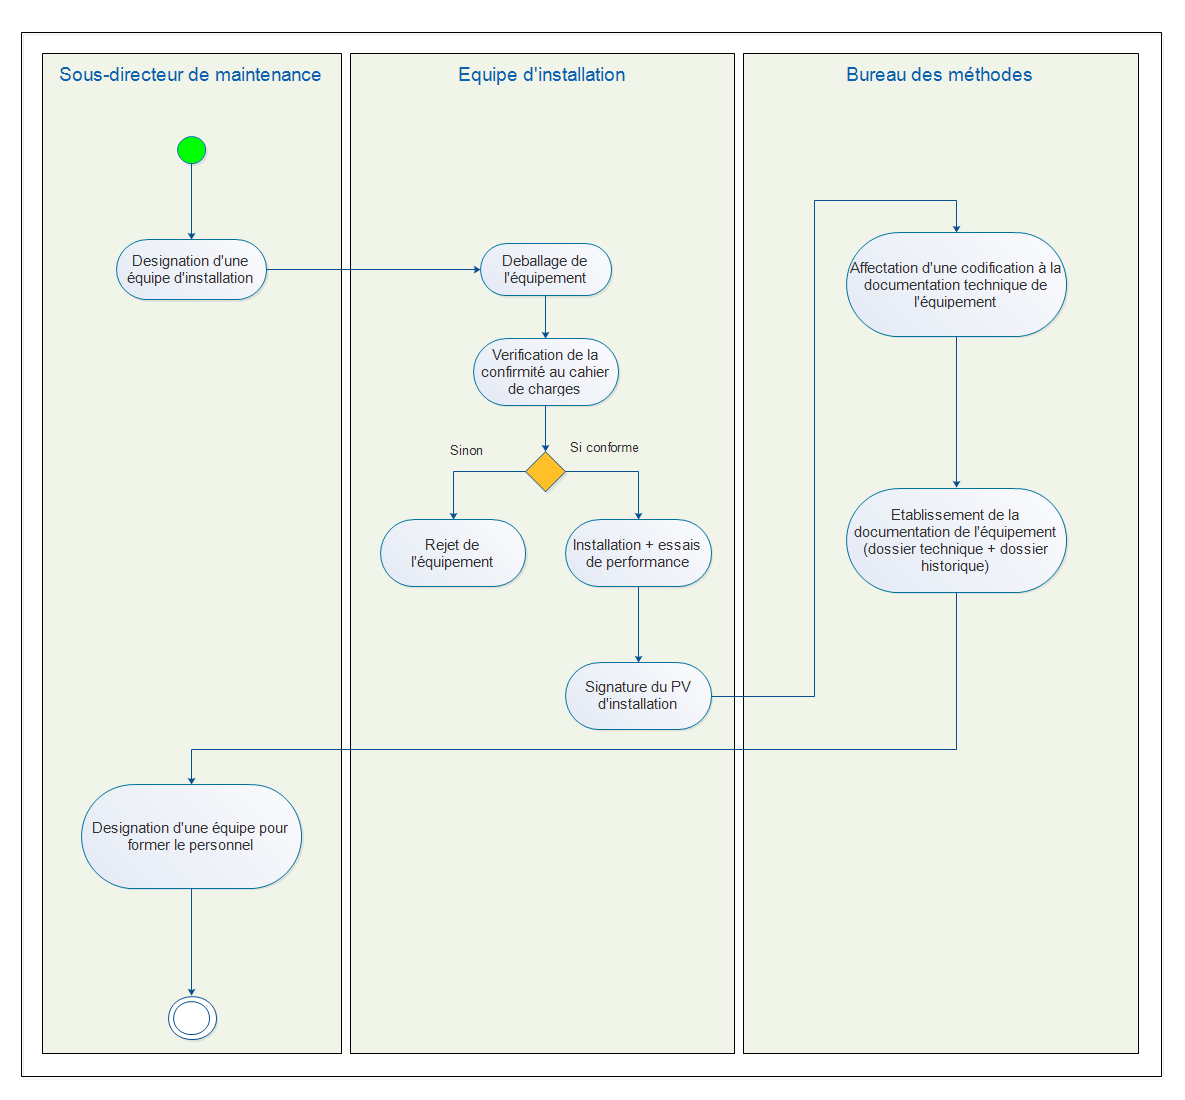
\includegraphics[width=1\linewidth]{./image_chapitre3/procedure_02}
	\caption[Proc�dure d'installation d'un nouvel �quipement]{Proc�dure d'installation d'un nouvel �quipement}
	\label{fig:procedure_02}
\end{figure}
\subsubsection*{Proc�dure 03: D�clenchements et r�ception des travaux de sous-traitance}
Le but est de s'assurer de la bonne qualit� des travaux en mati�re de sous-traitance. Elle s'applique � tous les travaux d'usinage, d'�lectricit� et d'�lectrom�canique.
\subsubsection*{Acteurs}
\begin{itemize}
	\item Sous-directeur de maintenance.
	\item Service des m�thodes.
	\item Service commercial.
\end{itemize}
\subsubsection*{Description de la proc�dure}
Cette proc�dure est d�clench�e d�s qu'une des structures �met une demande de r�paration et juge l'utilit� de faire appel � une sous-traitance.
\begin{enumerate}
	\item La sous-direction de maintenance re�oit la demande de r�paration. Si le montant de la r�paration est sup�rieur � 1 million de dinars, un cahier des charges doit �tre �tabli et sera transmis � la cellule juridique pour le traitement.
	\item la sous-direction de maintenance �tablit un courrier technique (�ventuellement un cahier des charges) et le remet au service commercial pour la consultation.
	\item Apr�s ouverture des plis par la commission d'achat, la sous-direction de maintenance �tablit un TCO\footnote{Tableau Comparatif des Offres} pour le choix du prestataire et le remet � la commission d'achat pour l'attribution.
	\item apr�s attribution, le chef du service m�thode �tablit une demande d'achat pour le service commercial pour l'�tablissement d'un bon de commande.
	\item Apr�s conclusion des travaux de maintenance par le prestataire, le bureau des m�thodes �tablit un rapport d�taill� des op�rations r�alis�es ainsi qu'une attestation des travaux faits.
	\item Apr�s r�ception de la facture de la part du prestataire, le directeur de maintenance �tablit un accus� de r�ception et la remet au service commercial pour l'�tablissement de la demande de paiement. Le dossier sera ensuite envoy� au service comptabilit�. 
\end{enumerate}
\newpage
Ci-dessous, un sch�ma qui illustre cette proc�dure:
\begin{figure}[H]
	\centering
	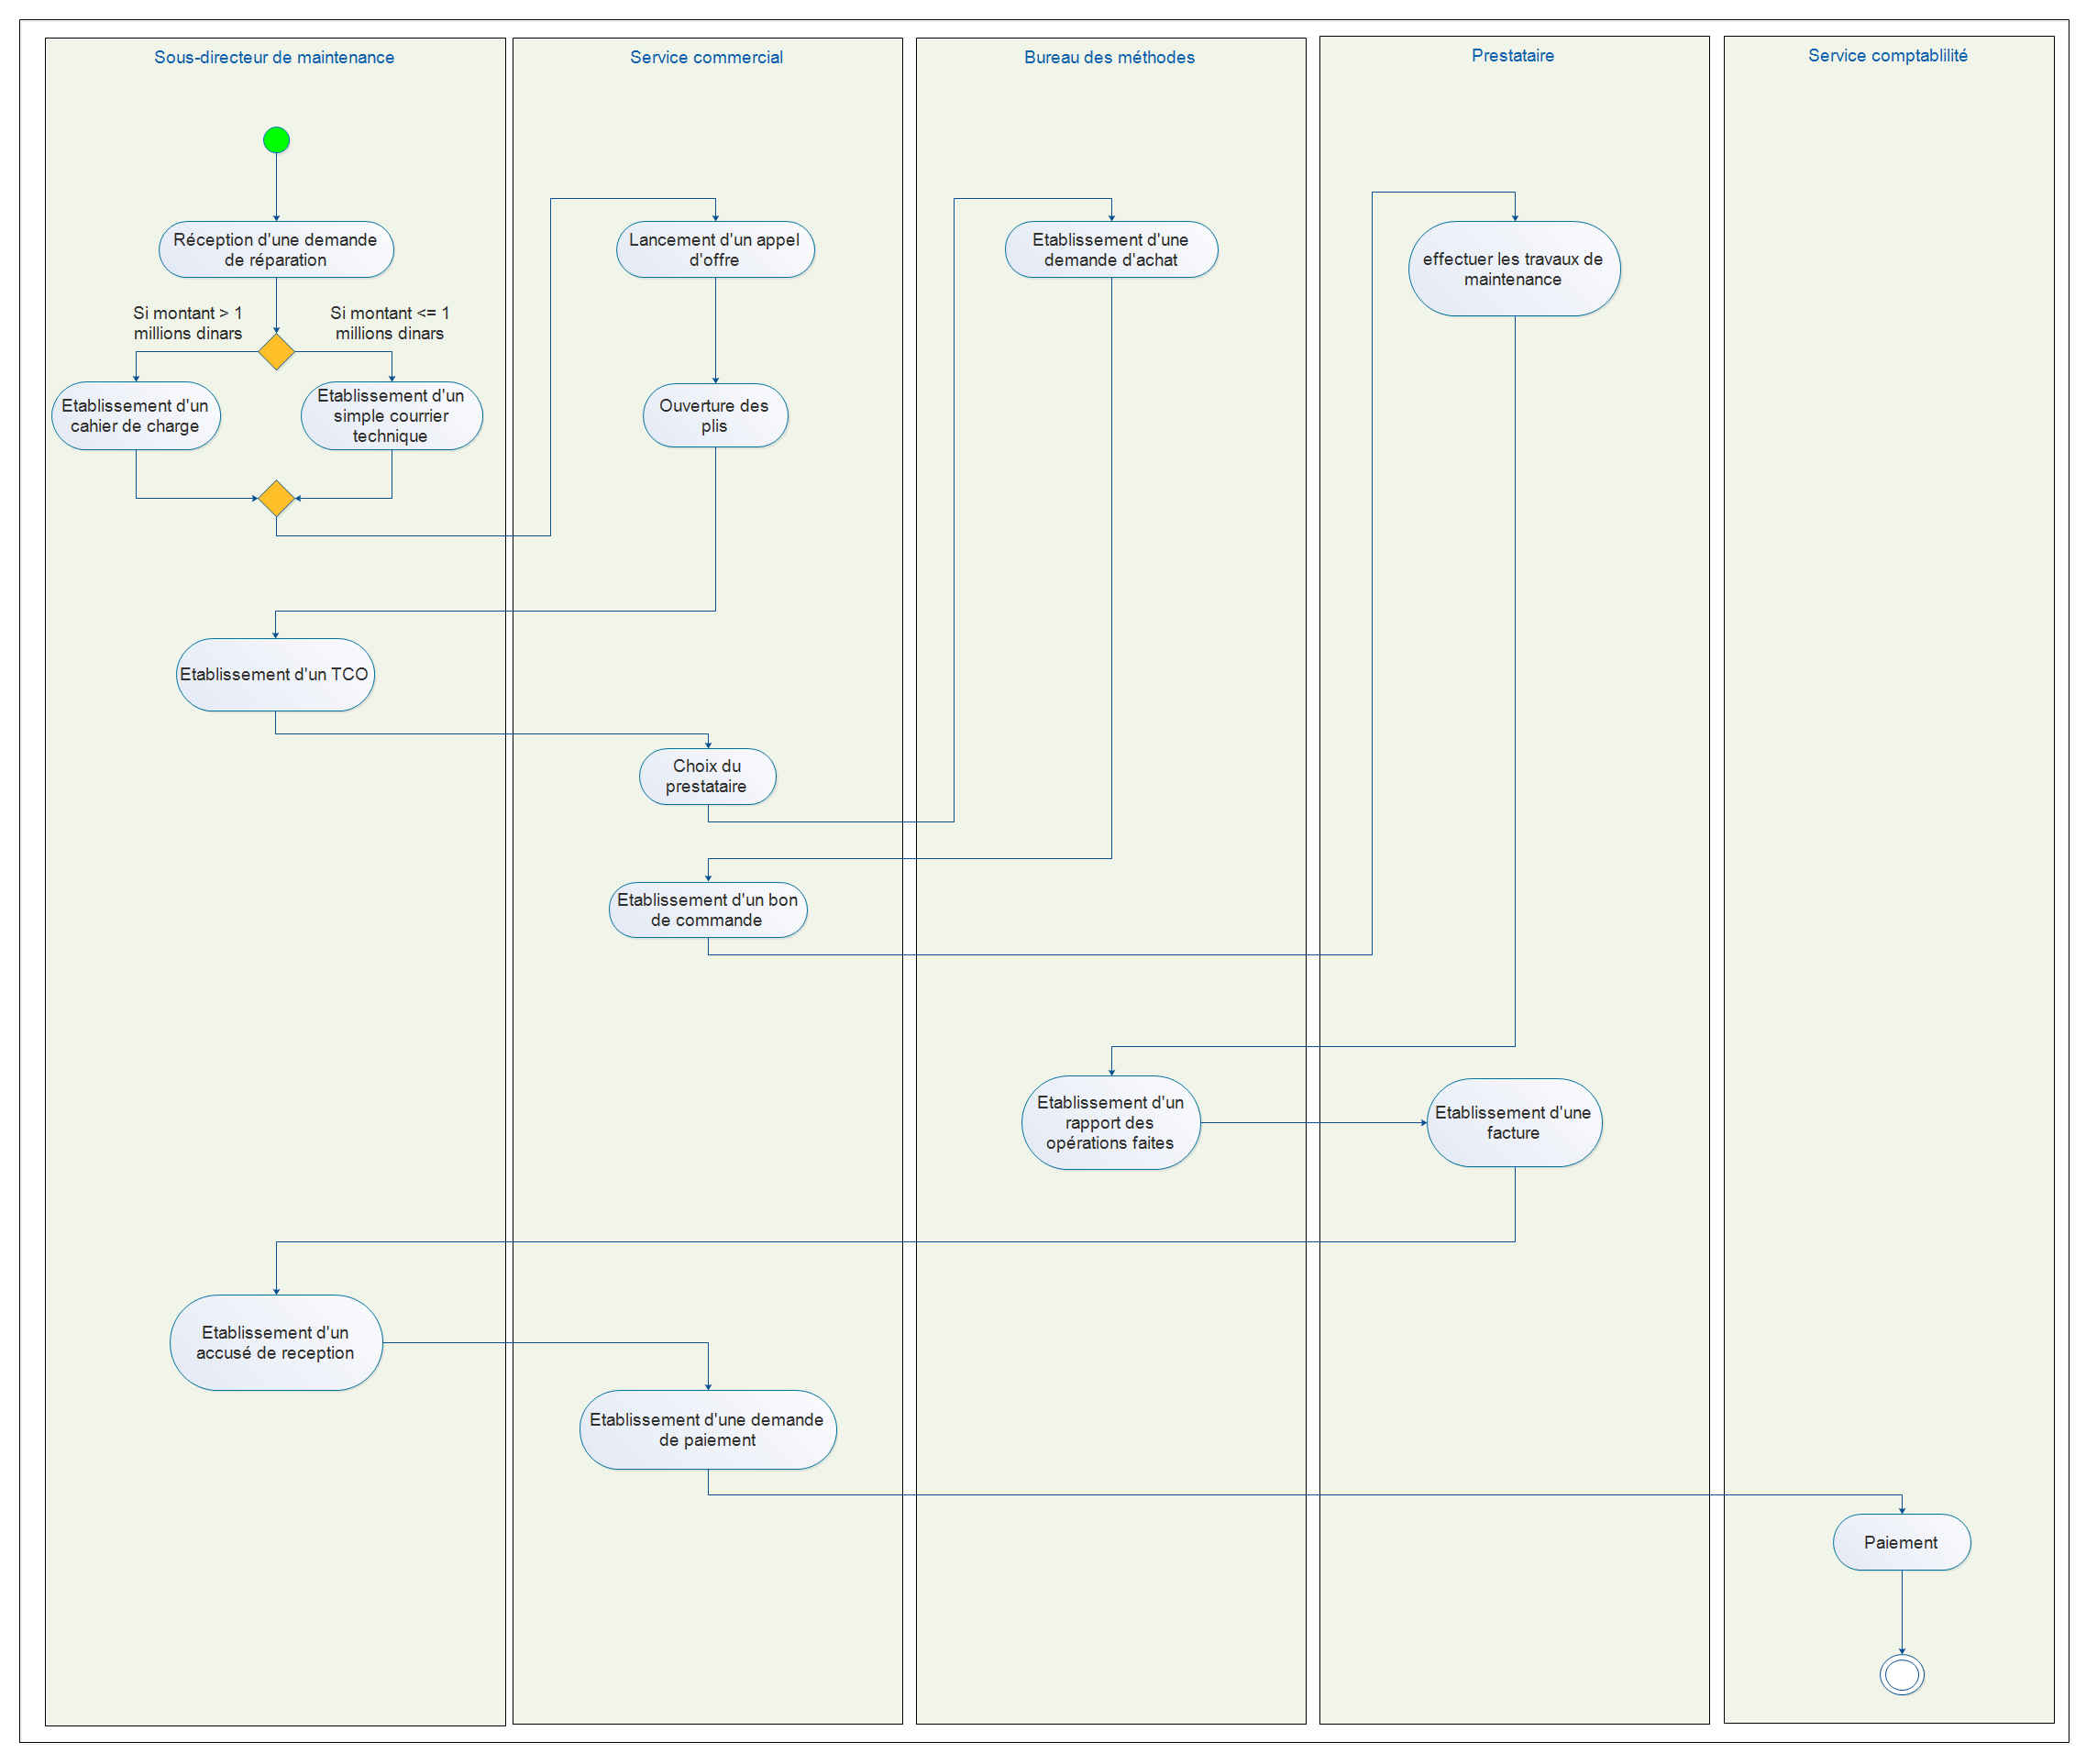
\includegraphics[width=1\linewidth]{./image_chapitre3/procedure_03}
	\caption[Proc�dure de d�clenchements et r�ception des travaux de sous-traitance]{Proc�dure de d�clenchement et r�ception des travaux de sous-traitance}
	\label{fig:procedure_03}
\end{figure}
\subsubsection*{Proc�dure 04: R�forme des �quipements}
Le but est de renouveler le parc machine pour des raisons de rentabilit�, �conomiques et de s�curit�. Elle s'applique � l'ensemble des �quipements de production. Les �quipements � r�former sont les ceux :
\begin{itemize}
	\item Ne r�pondant plus aux exigences technologiques (faible cadence, faible rendement, technologie d�pass�e, etc ....)
	\item Ne r�pondant plus aux normes pharmaceutiques en vigueur.
	\item Ne r�pondant plus aux normes s�curitaires.
	\item Dont les d�penses de r�paration d�passent 40 \% du prix d'acquisition.
\end{itemize}
\subsubsection*{Acteurs}
\begin{itemize}
	\item Direction de l'usine.
	\item Sous-direction de maintenance.
	\item D�partement de production.
	\item Service patrimoine.
\end{itemize}
\subsubsection*{Description de la proc�dure}
\begin{enumerate}
	\item La sous-direction de maintenance et la direction de la production proc�dent � un recensement des �quipements � r�former et �tablissent un rapport de r�forme qui sera transmet � la direction de l'usine pour convoquer la commission de r�forme. Une copie du PV de la r�union sera remise au d�partement de maintenance et une autre copie pour le service patrimoine.
	\item Le charg� des m�thodes retire l'�quipement en question de la liste des �quipements et archive son dossier historique et technique.
	\item Il �tablit un ordre de d�sinstallation et le remet � la direction de l'usine et au service patrimoine.
	\item D�sinstallation de l'�quipement en question.
\end{enumerate}
\subsubsection*{Proc�dure 05: Achat de la pi�ce de rechange}
Le but de cette proc�dure est d'assurer la disponibilit� de la pi�ce de rechange pour les �quipements. Elle s'applique � l'ensemble des �quipements et des utilit�s.
\subsubsection*{Acteurs}
\begin{itemize}
	\item Chef du service m�thodes.
\end{itemize}
\subsubsection*{Description de la proc�dure}
\begin{enumerate}
	\item Le chef du service m�thode consulte p�riodiquement l'�tat du stock de la PDR. 
	\item D�clencher l'op�ration d'achat pour les PDR dont les stocks sont au minimum.
	\item \textbf{L'op�ration d'achat:}
	\begin{itemize}
		\item Pour la PDR dont le montant ne d�passe pas 100 000 DA, consulter le fournisseur local pour avoir une facture proforma puis transmettre la demande d'achat au service commercial pour �tablir le bon de commande.
		\item Pour la PDR dont le montant d�passe 100 000 DA, on exige 3 factures proforma pour �tablir un TCO pour le choix du fournisseur (m�me proc�dure que pour la sous-traitance).
	\end{itemize}
	
\end{enumerate}
\subsubsection*{Proc�dure 06: Planification et r�alisation de la maintenance pr�ventive}
Le but est d'assurer une bonne planification pour la r�alisation des travaux de maintenance pr�ventive afin d'am�liorer la rentabilit� des �quipements de production.
\subsubsection*{Acteurs}
\begin{itemize}
	\item Chef du d�partement gestion des �quipements.
	\item Chef du d�partement interventions.
	\item Chef du service m�thodes.
	\item Sous-directeur de la maintenance. 
	\item Directeur de production.	
\end{itemize}
\subsubsection*{Description de la proc�dure}
\begin{enumerate}
	\item �tablir un planning pr�ventif des �quipements et un planning des travaux pr�ventifs pour chaque �quipement sur la base de la documentation technique et l'analyse des dossiers historiques des �quipements. 
	\item Recenser et v�rifier la disponibilit� de la PDR n�cessaire � l'ex�cution du planning. En cas d'indisponibilit� de la PDR, d�clencher l'op�ration d'achat.
	\item Programmer le planning des �quipements en fonction des p�riodes d'arr�t des machines.
	\item �tablir et transmettre une demande de r�paration accompagn�e du planning des travaux pr�ventifs de l'�quipement au chef de service d'intervention m�canique ou �lectrique. Ce dernier les transmettra � son tour � l'agent de maitrise (celui qui effectuera la r�paration).
	\item L'agent de maitrise ex�cute l'intervention et proc�de aux essais n�cessaires.
	\item Sur la demande de r�paration, il signale le service fait et le transmet au chef de service m�canique/�lectrique qui le signe et le transmet au chef de service m�thodes.
	\item Le chef de service m�thodes met � jour les dossiers historiques et �tablit un rapport d'activit�s des travaux pr�ventifs.
\end{enumerate}
\newpage
Ci-dessous, un sch�ma qui illustre cette proc�dure:
\begin{figure}[H]
	\centering
	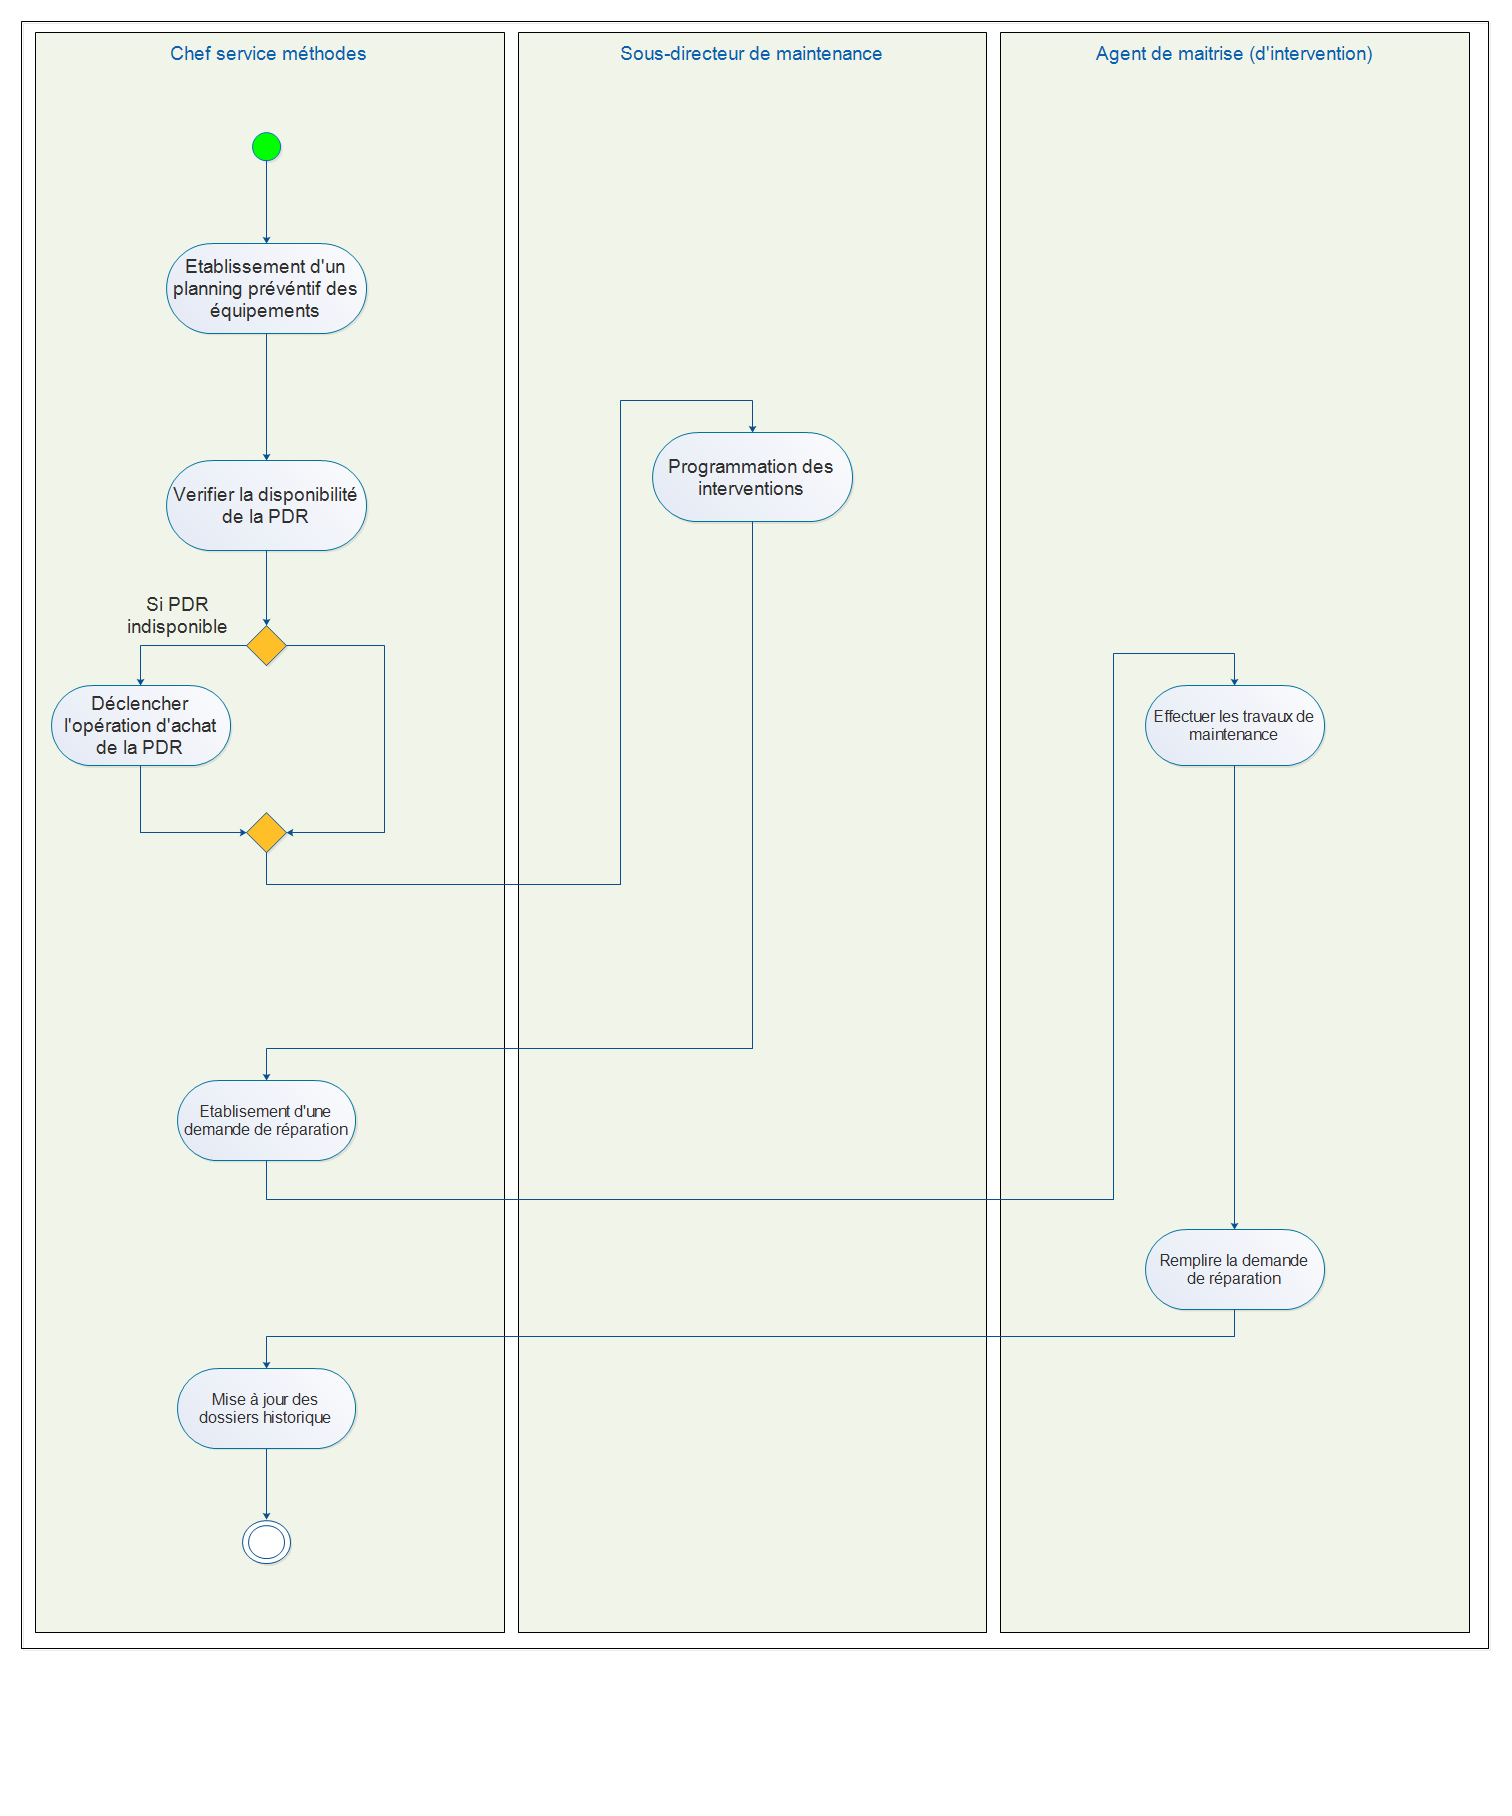
\includegraphics[width=1\linewidth]{./image_chapitre3/procedure_06}
	\caption[Planification et r�alisation de la maintenance pr�ventive]{Planification et r�alisation de la maintenance pr�ventive}
	\label{fig:procedure_06}
\end{figure}
\subsubsection*{Proc�dure 07: Ordonnancement et r�alisation de la maintenance curative}
Le but est de r�duire le temps d'arr�t des �quipements en organisant les interventions de maintenance.
\subsubsection*{Acteurs}
\begin{itemize}
	\item Chef de service m�thodes.
	\item Chef de d�partement concern� par la maintenance.
	\item Responsable du magasin.
	\item Technicien.	
\end{itemize}
\subsubsection*{Description de la proc�dure}
Cette proc�dure est d�clench�e d�s qu'une des structures �met une demande de r�paration.
\begin{enumerate}
	
	\item D�terminer la d�faillance et l'urgence d'intervention. S'il y a urgence, l'intervention sera imm�diate, sinon proc�der � sa programmation.
	\item Le chef du service m�thodes d�signe l'�quipe d'intervention.
	\item Pr�parer la pi�ce de rechange tout en visant le bon de sortie �tabli par le responsable du magasin.
	\item L'�quipe d'intervention proc�de � l'intervention. Une fois la r�paration effectu�e, le technicien effectue des essais en pr�sence du responsable du service concern� qui doit viser la demande de r�paration,il doit, aussi, remplir l'�tat des arr�ts journaliers. En cas de non-conformit� des essais, revoir et chercher la d�faillance.
	\item Le technicien remet la demande de r�paration ainsi que le bon de sortie pi�ce au bureau m�thodes.
	\item Le charg� des m�thodes mis a jour le dossier historique de l'�quipement concern� par la r�paration et rempli le rapport d'activit�s. 	
\end{enumerate}
Ci-dessous, un sch�ma qui illustre cette proc�dure:
\newpage
\begin{figure}[H]
	\centering
	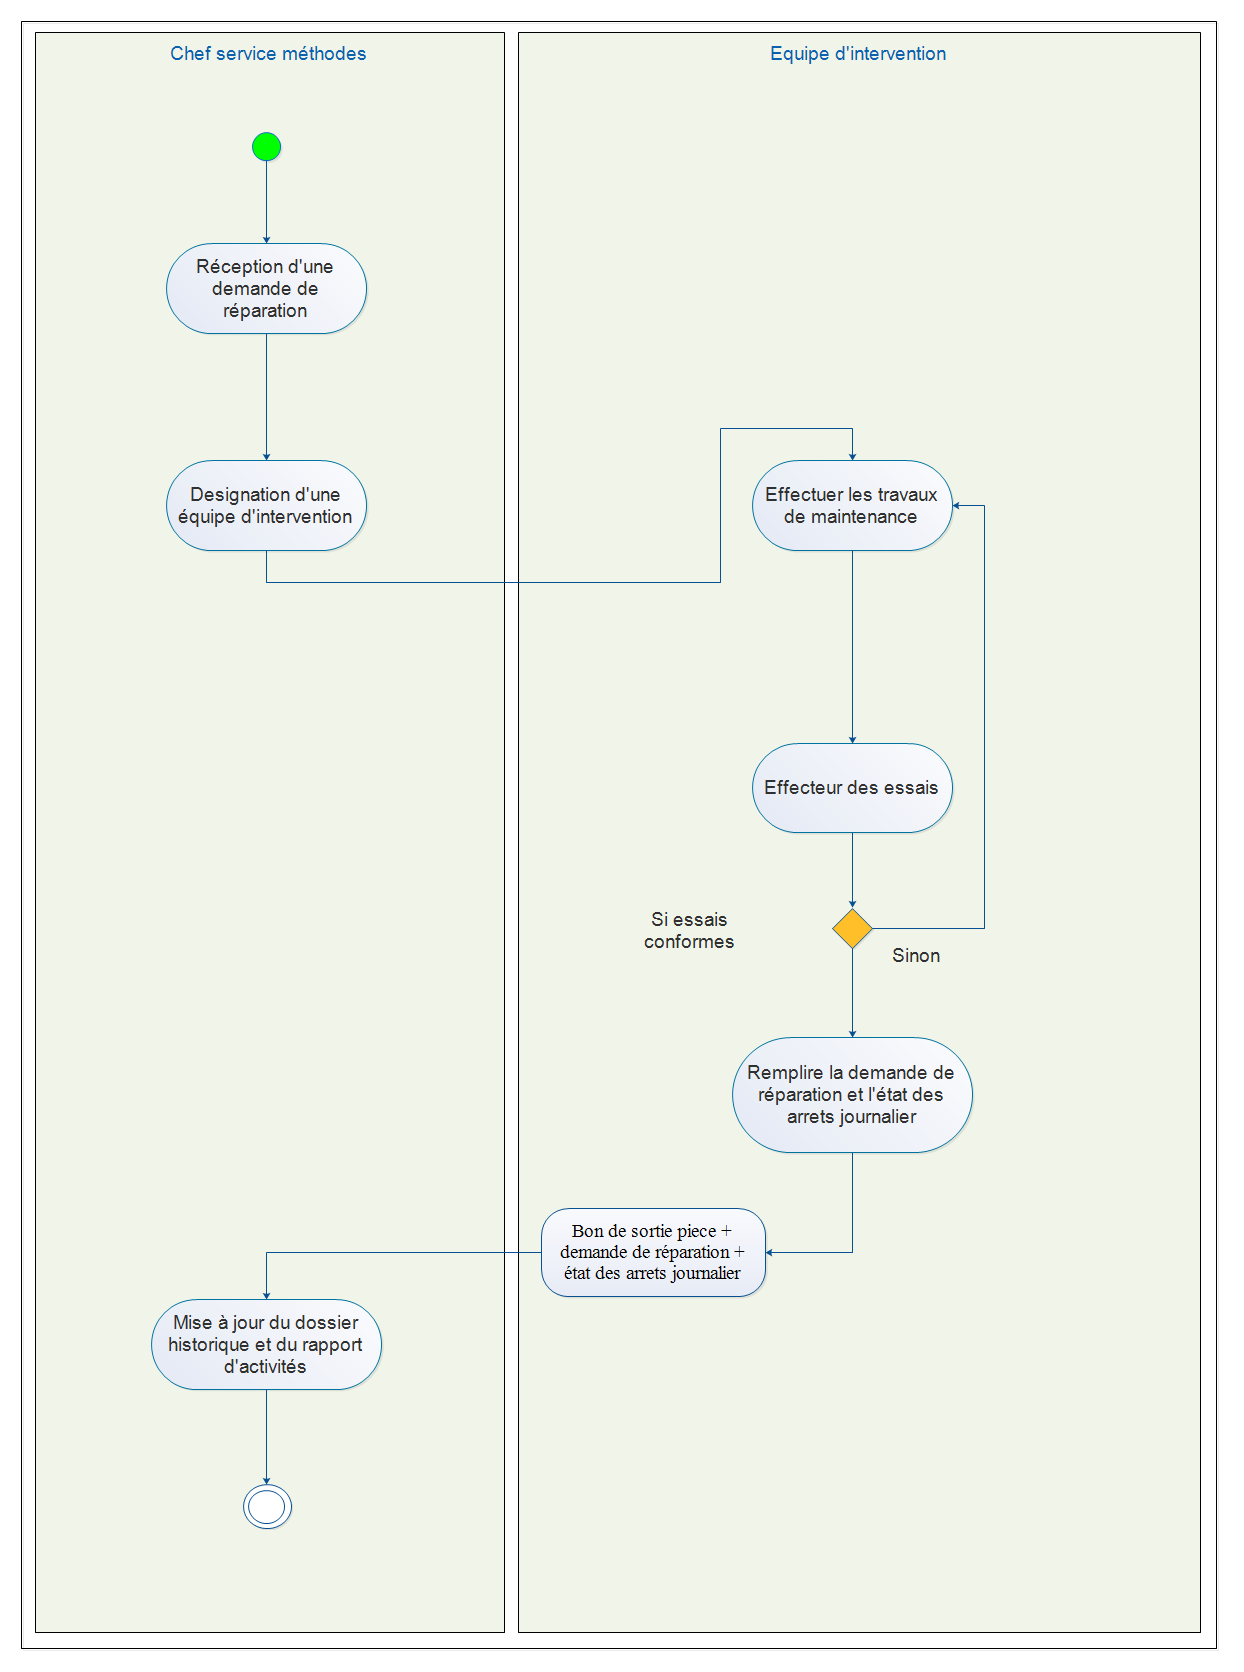
\includegraphics[width=1\linewidth]{./image_chapitre3/procedure_07}
	\caption[Ordonnancement et r�alisation de la maintenance curative]{Ordonnancement et r�alisation de la maintenance curative}
	\label{fig:procedure_07}
\end{figure}


\subsection{�tude de la codification existante}
La codification est l'op�ration qui consiste remplacer une information sous sa forme naturelle par un code clair et unique qui serait mieux adapt� aux besoins de l'utilisateur de l'information. \cite{web07}\\[0.5\baselineskip]
Un code est un nom abr�g� ou une repr�sentation de l'information permettant de d�signer un objet ou un concept de mani�re claire et unique.\cite{web07}\\[0.5\baselineskip]
Dans notre �tude de codification pour la sous-direction de maintenance, nous allons nous int�resser de la codification des �quipements et des pi�ces de rechange.  

\subsubsection*{Codification des �quipements}
Cette codification est structur�e comme suit :
\begin{figure}[H]
	\centering
	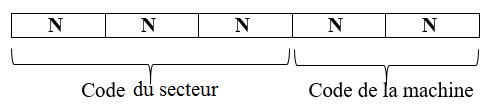
\includegraphics[width=0.4\linewidth]{./image_chapitre3/codification}
	%\caption[Proc�dure d'installation d'un nouvel �quipement]{Proc�dure d'installation d'un nouvel �quipement}
	\label{fig:codification}
\end{figure}
La codification des diff�rents secteurs de production est d�finie dans le tableau ci-dessous. Par contre, le code de la machine est un num�ro s�quentiel. 
\begin{center}
	\begin{tabular}{|p{3cm}|p{11.5cm}|}
		\hline
		\textbf{Code} & \textbf{Secteur}  \\
		\hline
		 000 &  P�teux  \\
		 \hline
		 040 &   Secs (fabrication)\\
		 \hline
		 050 &   Secs (pr�paration)\\
		 \hline
		 080 &  Sels \\
		 \hline
		 100 &  Sirops \\
		 \hline
		 140 &   Drag�ification\\
		 \hline
		 170 &   Pr�-conditionnement\\
		 \hline
		 200 &   Conditionnement\\
		 \hline
		 240 &  Pes�es  \\
		 \hline
		 250 &  Impression \\
		 \hline
		 300 &   Utilit�s (traitement d'air)\\
		 \hline
		 310 &  Utilit�s (traitement d'eaux et de vapeur) \\
		 \hline
		 320 &  Utilit�s (HVAC) \\
		 \hline
		 500 &  Installation commune (Conditionnement) \\
		 \hline
		 510 &  Installation commune (Production) \\
		 \hline
		 520 &  Installation commune (Maintenance) \\
		 \hline
		 550 &  Installation (Magasins et produits finis) \\
		 \hline
		 700 &  Direction \\
		 \hline
		 800 &  Production \\
		 \hline
		 900 & Laboratoire physico-chimie  \\
		 \hline
		 901 &  Laboratoire analytique \\
		 \hline
		 902 &  Laboratoire microbiologie \\
		 \hline
		 903 & Laboratoire in process  \\
		  \hline		
		
	\end{tabular} \\
	\captionof{table}{Codification des ateliers}
	\label{tab10}
\end{center}

 

\subsubsection*{Codification des documents}
Que ce soit pour le dossier technique, le dossier historique, la demande de r�paration, le planning des travaux pr�ventifs, le planning pr�ventif des �quipements, le bon de sortie des pi�ces ou l'�tat des arr�ts journaliers, la codification est repr�sent�e par un num�ro s�quentiel, ce qui rend la codification non significative.
\subsubsection*{Synth�se de la codification}
Durant notre �tude de la codification, nous avons constat� une codification non significative de tous les documents qui circulent dans le service de la maintenance. Or il est imp�ratif que SAIDAL leur mette en place une codification puissante afin de les suivre dans le processus de la maintenance.\\[0.5\baselineskip]
La codification utilis�e pour les �quipements est mal con�ue puisque nous en avons recens� quelques probl�mes, et qui sont :
\begin{itemize}
	\item Le nombre d'ateliers est de 24, cela veut dire que nous pouvons les repr�senter seulement sur 2 caract�res au lieu de 3 caract�res.
	\item Le nombre de machines dont dispose les ateliers voisine les cents, ce qui implique de pr�voir des codes pour tenir compte de l'�volution des �quipements � codifier. Cela peut �tre r�gl� par l'ajout d'un caract�re pour cette zone (descripteur).
\end{itemize}

\subsection{�tude quantitative}
Afin de donner une id�e sur les activit�s de la maintenance au niveau du groupe SAIDAL, nous avons r�alis� une �tude statistique. Nous pr�senterons le nombre d'interventions, les dur�es d'interventions, les temps d'arr�t des �quipements et le co�t des interventions pour chaque secteur de production pendant une p�riode d'un mois. Pour cela, nous avons utilis� les rapports d'activit� mensuels des dix premiers mois de l'ann�e 2015. Notons que cette �tude comprend � la fois les travaux de maintenance curative, pr�ventive et les travaux de sous-traitance vu qu'il n'existe pas des statistiques s�par�es pour chaque type d'intervention au niveau du service maintenance. 
\subsubsection*{Nombre d'interventions}
Le tableau ci-dessous pr�sente les nombre d'interventions mensuelles pour chaque secteur de production.
\begin{center}
	\begin{tabular}{|c|c|c|c|c|c|c|c|c|c|c|}
		\hline
		\multicolumn{3}{|c|}{Par sp�cialit�} & \multicolumn{8}{|c|}{Par secteur} \\
		\hline
		Elect. & M�can. & Utilit�s & Cdt & Divers & Sirops & Labo. & P�teux & Secs & Sels & Utilit�s \\  
		\hline
		33 & 155 & 15 & 36 & 12 & 52 & 1 & 19 & 62 & 17 & 4 \\  
		\hline			
		
	\end{tabular} \\
	\captionof{table}{Nombre d'interventions par mois}
	\label{tab11}
\end{center}
\noindent \textbf{Nombre moyen d'interventions par mois:} 203

\begin{figure}[H]
	\centering
	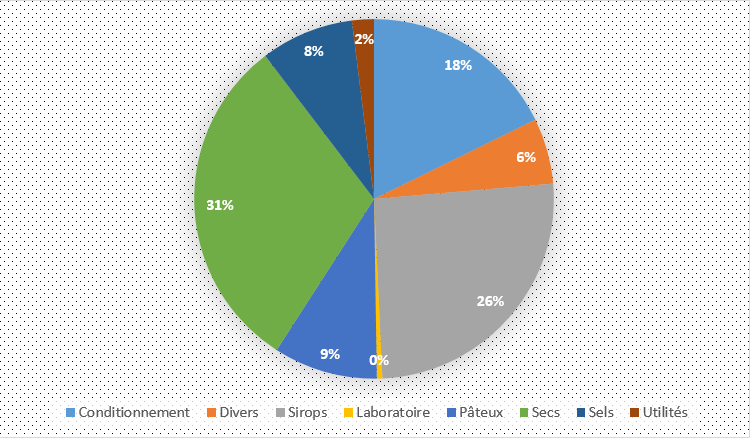
\includegraphics[width=0.9\linewidth]{./image_chapitre3/nombre_interventions}
	\caption[Nombre d'interventions par mois]{R�partition des interventions par atelier de production}
	\label{fig:nombreinterventions}
\end{figure}
\subsubsection*{Dur�es d'interventions}
Les tableaux ci-dessous pr�sente les dur�es d'interventions.
\begin{center}
	\begin{tabular}{|p{4cm}|p{4cm}|p{4cm}|}
		\hline
		Electrique & M�canique & Utilit�s  \\  
		\hline
		36h & 345h & 16h  \\  
		\hline	
	\end{tabular} \\
	\captionof{table}{Dur�e d'interventions par sp�cialit�}
	\label{tab12}
\end{center}

\begin{center}
	\begin{tabular}{|p{3cm}|p{3cm}|p{3cm}|p{3cm}|}
		\hline
		Secs/Sels & Sirops & P�teux & Utilit�s  \\  
		\hline
		276h & 46h & 30h & 45h  \\  
		\hline	
	\end{tabular} \\
	\captionof{table}{Dur�e d'interventions par secteur}
	\label{tab13}
\end{center}

\subsubsection*{Temps d'arr�t des �quipements}
Le tableau ci-dessous pr�sente le temps d'arr�t des �quipements pour chaque ateliers.
\begin{center}
	\begin{tabular}{|p{4cm}|p{4cm}|p{4cm}|}
		\hline
		Secs/Sels & Sirops & P�teux   \\  
		\hline
		284h & 60h & 34h  \\  
		\hline	
	\end{tabular} \\
	\captionof{table}{Temps d'arr�t des �quipements}
	\label{tab14}
\end{center}

\subsubsection*{Co�t d'intervention}
Le tableau ci-dessous pr�sente les co�ts d'interventions mensuelles par atelier de production et par sp�cialit�.
\begin{center}
	\begin{tabular}{|p{2.3cm}|c|c|c|c|c|c|c|c|c|}
		\hline
		& Cdt & Divers & Sirops & Labo. & P�teux & Secs & Sels & Utilit�s & \textbf{TOTAL}   \\
		\hline
		main d'\oe uvre �lectrique & 1983 & 1327 & 172 & / & 1444.5 & 2106 & 951 & / & \textbf{7983.5} \\
		\hline
		main d'\oe uvre m�canique & 21576 & 4957 & 10702 & / & 8164.5 & 26706 & 8282.5 & / & \textbf{80388} \\
		\hline
		main d'\oe uvre utilit�s & 154 & 693 & 231 & 385 & 77 & 77 & / & 688.5 & \textbf{2305.5} \\
		\hline
		\textbf{TOTAL} & \textbf{23713} & \textbf{6977} & \textbf{11105} & \textbf{385} & \textbf{9686} & \textbf{28889} & \textbf{9233.5} & \textbf{689.5} & \textbf{90677} \\		 
		\hline	
	\end{tabular} \\
	\captionof{table}{Cout d'intervention}
	\label{tab15}
\end{center}
\subsection{Nomenclature des �quipements}
La nomenclature des �quipements est un document n�cessaire dans le service de maintenance d'une entreprise, comme nous l'avons cit� dans le chapitre pr�c�dent, or le groupe SAIDAL ne dispose pas actuellement d'une nomenclature pour ses �quipements.  
\subsection{Analyse de la situation informatique}
Le service maintenance du groupe SAIDAL ne dispose ni d'infrastructure r�seau ni base de donn�es. En effet, la gestion de maintenance se fait exclusivement sur des fichiers EXCEL. L� encore, un grand manque se pr�sente car seuls les rapports d'activit�s mensuels sont concern�s, les autres documents sont g�r�s manuellement (sur papier).
\subsection{Diagnostic de l'existant}
Le diagnostic est n�cessaire avant tout d�veloppement d'une application et toute prise de d�cision au sein d'une organisation. Il s'agit de d�finir les probl�mes du processus existant ainsi que les causes de dysfonctionnement et les cons�quences qui en r�sultent.\\[0.5\baselineskip]
L'�tude des documents, des postes de travail, des proc�dures de travail, de la codification existante et la situation informatique nous a permis de recenser un certain nombre d'anomalies
relevant de la gestion de la maintenance au niveau du groupe.\\[0.5\baselineskip]
Dans notre diagnostic, nous proc�derons comme suit:
\begin{itemize}
	\item Dresser une liste des diff�rentes anomalies d�tect�es.
	\item Recenser les causes de chaque anomalie et les cons�quences qu'elle peut engendrer.
	\item enfin, proposer une/des solutions pour chaque anomalie.
\end{itemize}
\noindent \textbf{Anomalie 01: }Nombreuses informations des documents ne sont pas utilis�es.\\[0.5\baselineskip]
\noindent Causes:
\begin{itemize}
	\item Ambigu�t� des informations pr�sent�es dans les diff�rents documents manipul�s dans le processus de la maintenance (documents inadapt�s).
\end{itemize}
\noindent Cons�quences:
\begin{itemize}
	\item Perte d'informations et de temps.
	\item Redondance de l'information.
\end{itemize}

\noindent Suggestions:
\begin{itemize}
	\item Garder les informations principales et supprimer les autres.
\end{itemize}
\vspace{0.5cm}

\noindent \textbf{Anomalie 02: }Difficult� d'acc�der � l'information\\[0.5\baselineskip]
\noindent Causes:
\begin{itemize}
	\item Utilisation du support papier pour le suivi des diff�rentes proc�dures de travail et pour la r�daction des �tats journaliers et du rapport d'activit�s mensuel.
	\item Absence d'une base de donn�es centralis�e.
	
\end{itemize}
\noindent Cons�quences:
\begin{itemize}
	\item Perte de temps dans la recherche d'information.
\end{itemize}

\noindent Suggestions:
\begin{itemize}
	\item Utiliser un syst�me d'information avec une base de donn�e centralis�e.
	\item Automatiser les proc�dures de la maintenance.	
\end{itemize}
\vspace{0.5cm}
\noindent \textbf{Anomalie 03: }quelques informations sont obsol�tes\\[0.5\baselineskip]
\noindent Causes:
\begin{itemize}
	\item Existence des documents qui ne sont pas mis � jour.
	\item Existence des documents qui ne sont pas approuv�s.
	\item Existence des documents qui ne sont pas dat�s.
	
\end{itemize}
\noindent Cons�quences:
\begin{itemize}
	\item Incoh�rence des r�sultats puisque le service de la maintenance se r�f�re � des informations qui ne sont pas actualis�es.
\end{itemize}

\noindent Suggestions:
\begin{itemize}
	\item Mettre � jour, approuver et dater tous les documents manipul�s dans le processus de la maintenance	
\end{itemize}
\newpage
\noindent \textbf{Anomalie 04: }incoh�rence de rattachement du magasin\\[0.5\baselineskip]
\noindent Causes:
\begin{itemize}
	\item Le magasin appartient � la direction de la gestion des stocks, alors qu'il contient principalement la PDR qui est cens�e utilis�e par la sous-direction de la maintenance.
	
\end{itemize}
\noindent Cons�quences:
\begin{itemize}
	\item Chevauchements des responsabilit�s entre la sous-direction de la maintenance et la direction de la gestion des stocks.        
	\item Lenteur dans l'affectation de la pi�ce de rechange.
	
\end{itemize}

\noindent Suggestions:
\begin{itemize}
	\item Attacher le magasin � la sous-direction de la maintenance.
\end{itemize}
\vspace{0.5cm}
\noindent \textbf{Anomalie 05: }incoh�rence de rattachement du service des projets neufs\\[0.5\baselineskip]
\noindent Causes:
\begin{itemize}
	\item Le service Projets Neufs qui figure dans l'organigramme de la sous-direction de la maintenance et plus exactement dans le d�partement des interventions, ne fait objet d'aucune t�che ou mission relative au processus de la maintenance.
	
\end{itemize}
\noindent Cons�quences:
\begin{itemize}
	\item Officiellement, le personnel du service des projets neufs participe dans le processus de la maintenance, pourtant il ne le fait pas r�ellement.
	\item Difficult� dans la recherche de l'information.
	
\end{itemize}

\noindent Suggestions:
\begin{itemize}
	\item Attacher le service des projets neufs � la direction des moyens g�n�raux.
\end{itemize}
\vspace{0.5cm}
\noindent \textbf{Anomalie 06: }existence des postes vacants\\[0.5\baselineskip]
\noindent Causes:
\begin{itemize}
	\item Les postes de travail existent mais le personnel ne leurs est pas affect�.
	
\end{itemize}
\noindent Cons�quences:
\begin{itemize}
	\item Plusieurs responsabilit�s ne sont pas assum�es.
	
\end{itemize}

\noindent Suggestions:
\begin{itemize}
	\item Cr�er les postes de travail quand il y en a vraiment besoin.	
\end{itemize}
\vspace{0.5cm}
\noindent \textbf{Anomalie 07: }absence de quelques fiches de postes\\[0.5\baselineskip]
\noindent Causes:
\begin{itemize}
	\item Sur un effectif total de 41 personnes, seulement 18 fiches de postes ont �t� �tablies.
	
\end{itemize}
\newpage
\noindent Cons�quences:
\begin{itemize}
	\item Existence des postes auxquels la sous-direction de la maintenance n'a pas attribu� les responsabilit�s et les t�ches.
	
\end{itemize}

\noindent Suggestions:
\begin{itemize}
	\item Elaborer les fiches de postes manquantes en d�finissant clairement leurs t�ches et responsabilit�s.	
\end{itemize}
\vspace{0.5cm}
\noindent \textbf{Anomalie 08: }La codification utilis�e sur certains documents est non significative.\\[0.5\baselineskip]
\noindent Causes:
\begin{itemize}
	\item La codification utilis�e ne respecte pas les caract�ristiques de la codification et qui sont la non ambig�it�, l'adaptation aux nouveaux besoins, la possibilit� d'extension et la concision.
	
\end{itemize}
\noindent Cons�quences:
\begin{itemize}
	\item Le classement et la recherche de ces documents deviennent une t�che fastidieuse.
	
\end{itemize}

\noindent Suggestions:
\begin{itemize}
	\item Mise en place d'une codification significative et puissante.	
\end{itemize}
\vspace{0.5cm}
\noindent \textbf{Anomalie 09: }Retard dans l'�tablissement des documents et l'accomplissement des t�ches de maintenance.\\[0.5\baselineskip]
\noindent Causes:
\begin{itemize}
	\item Des t�ches manuelles.
	\item Lourdeur de la circulation de l'information.
	\item La complexit� des proc�dures de travail. Par exemple la lenteur de l'op�ration d'achat de de la PDR vu qu'elle exige la participation de plusieurs acteurs au sein de l'entreprise et il n'existe aucun m�canisme qui permet d'assouplir cette op�ration en cas des pannes urgentes n�cessitant une PDR non pr�sente dans le magasin.
	
\end{itemize}
\noindent Cons�quences:
\begin{itemize}
	\item Perte de temps.
	\item Retard de l'intervention au moment voulu et le non respect des d�lais.	
\end{itemize}
\vspace{0.5cm}
\noindent \textbf{Anomalie 10: }Les t�ches de la maintenance pr�ventive sont ex�cut�es une fois par ann�e. \\[0.5\baselineskip]
\noindent Causes:
\begin{itemize}
	\item La maintenance pr�ventive est ex�cut� une fois par ann�e (pendant la p�riode de l'arr�t annuel) faute de coordination entre le service de maintenance et le service de production. 

\end{itemize}
\noindent Cons�quences:
\begin{itemize}
	\item Augmentation des pannes du mat�riel.
	\item Cumul de travail sur les maintenanciers.
	
\end{itemize}
\noindent Suggestions:
\begin{itemize}
	\item Ex�cuter les t�ches de maintenance r�guli�rement suivant un planning �tabli en coordination avec les services de production.
\end{itemize}
\vspace{0.5cm}
\noindent \textbf{Anomalie 11: }Manque d'informations sur le mat�riel\\[0.5\baselineskip]
\noindent Causes:
\begin{itemize}
	\item Absence d'une base de donn�es fiable et unifi�e des �quipements.
	\item Absence d'une nomenclature des �quipements.
	\item Les fiches techniques sont obsol�tes et parfois absentes.
	
\end{itemize}
\noindent Cons�quences:
\begin{itemize}
	\item Perte de temps.
	\item Informations relatives au mat�riel fauss�es ou perdu (ex : �tat du mat�riel, documents
	techniques, etc ....).
	\item Mauvais entretien des �quipements.
	
\end{itemize}
\noindent Suggestions:
\begin{itemize}
	\item �tablir des fiches techniques de tout le mat�riel et veiller � leurs mises � jour.
	\item �tablir une nomenclature des �quipements.	
\end{itemize}

\include{pagevide}

\chapter{\sc �tude conceptuelle }
\section{Introduction}
Apr�s avoir achev� l'�tude de l'existant qui nous a permis d'analyser le fonctionnement de la maintenance au sein du groupe SAIDAL et d'en d�duire les anomalies, les dysfonctionnements et les suggestions, et apr�s avoir �cout� les propositions de la sous-direction de la maintenance , nous abordons l'�tape suivante qui consiste � concevoir un syst�me de gestion de maintenance assist�e par ordinateur en passant par l'automatisation de l'ancien syst�me et en tenant compte des axes d'am�liorations propos�s.\\[0.5\baselineskip]
L'objectif de cette �tape est de d�terminer de fa�on d�taill�e et pr�cise ce que le syst�me devrait faire, afin de r�pondre � nos objectifs cit�s dans le premier chapitre.\\[0.5\baselineskip]
Pour notre conception, nous optons pour la mod�lisation orient�e objet UML qui sera pilot�e par la d�marche 2TUP.
� UML se d�finit comme un langage de mod�lisation graphique et textuel destin� � comprendre et d�crire des besoins, sp�cifier et documenter des syst�mes, esquisser des architectures logicielles, concevoir des solutions et communiquer des points de vue �.\cite{ref07}\\[0.5\baselineskip]
Sa stabilit� de mod�lisation, sa normalisation ainsi que la facilit� et la clart� de ses diagrammes ont fait d'UML un outil de choix pour notre mod�lisation.\\[0.5\baselineskip]
� 2TUP signifie � 2 Tracks Unified Process �, il apporte une r�ponse aux contraintes de changement continuel impos�es aux syst�mes d'information de l'entreprise. En ce sens, il renforce le contr�le sur les capacit�s d'�volution et de correction de tels syst�mes. � 2 Tracks � signifie litt�ralement que le processus suit deux chemins. Il s'agit des chemins � fonctionnel � et � d'architecture technique �, qui correspondent aux deux axes de changement impos�s au syst�me informatique �.\cite{ref08}\\[0.5\baselineskip]
la figure suivante repr�sente le sch�ma du processus 2TUP.\\[0.5\baselineskip]
\begin{figure}[H]
	\centering
	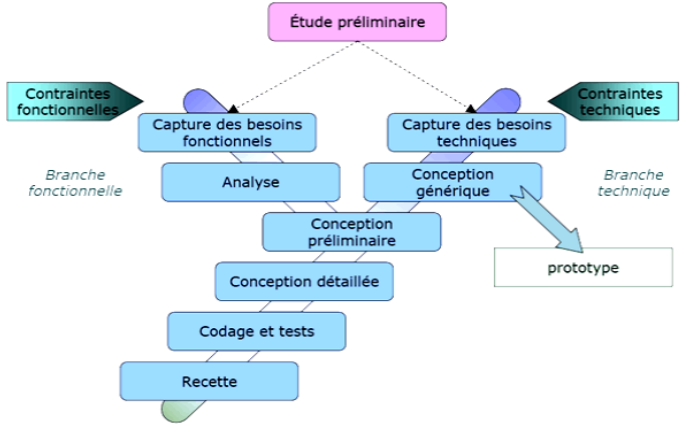
\includegraphics[width=0.9\linewidth]{./image_chapitre4/2TUP}
	\caption[Le processus de d�veloppement en Y (2TUP)]{Le processus de d�veloppement en Y (2TUP)}\cite{ref08}
	\label{fig:2TUP}
\end{figure}
\begin{itemize}
	\item \textbf{ La branche fonctionnelle (partie gauche) : }comporte la capture et l'analyse des besoins fonctionnels, qui produisent un mod�le des besoins focalis� sur le m�tier des utilisateurs.\cite{ref08}
	\item \textbf{ La branche technique (partie droite) : }comporte la capture des besoins techniques, qui recense toutes les contraintes et les choix dimensionnant la conception du syst�me, ainsi que la conception g�n�rique qui d�finit les composants n�cessaires � la construction de l'architecture technique.\cite{ref08}
	\item \textbf{ La branche du milieu  : }consiste � fusionner les r�sultats des 2 branches. Elle comporte la conception pr�liminaire, la conception d�taill�e, le codage et l'int�gration. Cette fusion conduit � l'obtention d'un processus en forme d'Y.\cite{ref08}
\end{itemize}

Le choix de cette d�marche n'est pas fortuit, mais ob�it � des consid�rations hautement professionnelles, notamment :
\begin{itemize}
	\item La compatibilit� avec UML.
	\item Chaque phase du processus 2TUP peut �tre d�compos�e en plusieurs it�rations.
	\item Chaque it�ration produit un incr�ment du produit.
\end{itemize}
\newpage
\section{ Etude pr�liminaire }

L'�tude pr�liminaire est la premi�re �tape du processus de d�veloppement, elle consiste � effectuer un premier rep�rage des besoins fonctionnels et techniques, en identifiant : \cite{ref08}
\begin{itemize}
	\item Les acteurs qui vont interagir avec le syst�me.
	\item Les messages qu'�changent les acteurs et le syst�me.
	\item Le diagramme du contexte.
\end{itemize}
\subsection{ Identification des acteurs  }
Les acteurs sont toute entit� externe (utilisateur humain, dispositif mat�riel ou autre syst�me) ayant une interaction directe avec le syst�me �tudi�. \cite{ref08}
\begin{figure}[H]
	\centering
	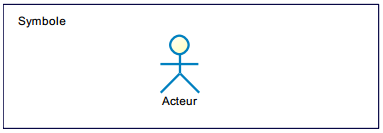
\includegraphics[width=0.9\linewidth]{./image_chapitre4/acteur}
	\caption[Repr�sentation d'un acteur dans l'UML]{Repr�sentation d'un acteur dans l'UML}
	\label{fig:acteur}
\end{figure}
L'�tude des documents et des proc�dures de travail effectu�e dans le chapitre �tude de l'existant et la prise en consid�ration des exigences et des propositions du groupe SAIDAL, nous ont permis de dresser une liste exhaustive des acteurs qui vont interagir avec le nouveau syst�me et leurs r�les comme la montre le tableau suivant :\\

\begin{center}
	\begin{tabular}{|p{3.5cm}|p{11cm}|}
		\hline
		\textbf{Acteur} &  \textbf{R�le}\\
		\hline
		\textbf{Administrateur} & 
		\begin{itemize}
			\item G�rer les utilisateurs, d�finir les profils et attribuer les privil�ges et les droits d'acc�s.
			\item S'occuper aussi de la maintenance
			du syst�me.			
		\end{itemize}\\
		\hline
		
\end{tabular} \\
\end{center}
\newpage
\begin{center}
	\begin{tabular}{|p{3.5cm}|p{11cm}|}
		\hline
		\textbf{Acteur} &  \textbf{R�le}\\
		\hline	
		\textbf{Chef du service de m�thodes} & 
		\begin{itemize}
			\item Recevoir les demandes de r�parations.
			\item �tablir les ordres de travail.
			\item Demander le PMP d'un �quipement.
			\item �tablir le planning pr�ventif des �quipements.		
			\item Retirer l'�quipement r�form� de la liste des �quipements.
			\item Demander des statistiques concernant la maintenance.
		\end{itemize}\\
		\hline
		\textbf{Chef du service de production} & 
		\begin{itemize}
			\item �tablir les demandes de r�paration.			
		\end{itemize}\\
		\hline
		\textbf{Chef du service �lectrique} & 
		\begin{itemize}
			\item Affecter l'ordre de travail aux intervenants (�lectriciens).
			\item Demander des statistiques de la maintenance concernant son service.			
		\end{itemize}\\
		\hline
		\textbf{Chef du service m�canique} & 
		\begin{itemize}
			\item Affecter l'ordre de travail aux intervenants (m�caniciens).
			\item Demander des statistiques de la maintenance concernant son service.			
		\end{itemize}\\
		\hline
		\textbf{Intervenant} & 
		\begin{itemize}
			\item Consulter le planning des
			interventions.
			\item Ex�cuter les interventions qui lui sont assign�es et remettre l'ordre de travail � son chef de service.			
		\end{itemize}\\
		\hline	
		\textbf{Syst�me de gestion des stocks} & 
		\begin{itemize}
			\item Envoyer au syst�me l'�tat des stocks de la PDR.			
		\end{itemize}\\
		\hline
	\end{tabular} \\
	\captionof{table}{Les acteurs et leurs r�les dans le syst�me }
	\label{tab16}
\end{center}

\newpage
\subsection{ Identification des messages  }
Les messages sont des communications unidirectionnelles entre objets transportant de l'information pour d�clencher un �v�nement chez le r�cepteur.  \cite{ref08}\\[0.5\baselineskip]
\textbf{Note : }Nous avons num�rot� les messages qui sont repr�sent�s dans le diagramme de contexte. Les num�ros attribu�s ne repr�sentent pas un ordre.\\[0.5\baselineskip]
Les deux tableaux suivants illustrent la liste des messages re�us et �mis par le nouveau syst�me :\\[0.5\baselineskip]
\textbf{Le syst�me re�oit les messages suivants : }

\begin{center}
	\begin{tabular}{|p{1.5cm}|p{3cm}|p{9.5cm}|}
		\hline
		\textbf{Num�ro} &  \textbf{Source} &  \textbf{Description} \\
		\hline
		\textbf{1} & Administrateur & Cr�er ou modifier les utilisateurs.\\
		\hline		
		\textbf{2} & Chef du service de production & Etablir une demande de r�paration.\\
		\hline			
		\textbf{3} & Chef du service de m�thodes & Cr�er des ordres de travail.\\
		\hline
		\textbf{4} & Chef du service de m�thodes & Demander le PMP d'un �quipement.\\
		\hline	
		\textbf{5} & Chef du service de m�thodes & Demander le planning pr�ventif des �quipements.\\
		\hline
		\textbf{6} & Chef du service de m�thodes & Demander des statistiques, ratios sur la maintenance.\\
		\hline
		\textbf{7} & Chef du service de m�thodes & Demander l'historique des interventions.\\
		\hline
		\textbf{8} & Chef du service �lectrique & Demander des statistiques concernant son service.\\
		\hline
		\textbf{9} & Chef du service �lectrique & Demander le planning pr�ventif des �quipements.\\
		\hline
		\textbf{10} & Chef du service m�canique & Demander des statistiques concernant son service.\\
		\hline
		\textbf{11} & Chef du service m�canique & Demander le planning pr�ventif des �quipements.\\
		\hline
		\textbf{12} & Intervenant & Demander le PMP d'un �quipement.\\
		\hline
		\textbf{13} & Intervenant & Demander le planning pr�ventif des �quipements.\\
		\hline
		\textbf{14} & Syst�me de gestion des stocks & Envoyer au syst�me l'�tat des stocks de la PDR.\\
		\hline
\end{tabular} \\
\captionof{table}{Liste des messages re�us par le syst�me }
\label{tab17}
\end{center}
\newpage

\textbf{Le syst�me �met les messages suivants :  }

\begin{center}
	\begin{tabular}{|p{1.5cm}|p{3cm}|p{9.5cm}|}
		\hline
		\textbf{Num�ro} &  \textbf{Destination} &  \textbf{Description} \\
		\hline	
		\textbf{15} & Chef du service de m�thodes & statistiques et ratios.\\
		\hline
		\textbf{16} & Chef du service de m�thodes & historique des interventions.\\
		\hline
		\textbf{17} & Chef du service de m�thodes & G�n�rer le PMP automatiquement.\\
		\hline
		\textbf{18} & Chef du service de m�thodes & G�n�rer le planning pr�ventif des �quipements automatiquement.\\
		\hline	
		\textbf{19} & Chef du service �lectrique & statistiques et ratios.\\
		\hline
		\textbf{20} & Chef du service �lectrique & G�n�rer le planning pr�ventif des �quipements automatiquement.\\
		\hline
		\textbf{21} & Chef du service m�canique & statistiques et ratios.\\
		\hline
		\textbf{22} & Chef du service m�canique & G�n�rer le planning pr�ventif des �quipements automatiquement.\\
		\hline
		\textbf{23} & Intervenant & G�n�rer le PMP automatiquement.\\
		\hline
		\textbf{24} & Intervenant & G�n�rer le planning pr�ventif des �quipements automatiquement.\\
		\hline
	\end{tabular} \\
	\captionof{table}{Liste des messages �mis  par le syst�me }
	\label{tab18}
\end{center}
\newpage

\subsection{ Diagramme de contexte  }
Le diagramme suivant repr�sente les messages �chang�s entre le nouveau syst�me d'information et les acteurs :
\begin{figure}[H]
	\centering
	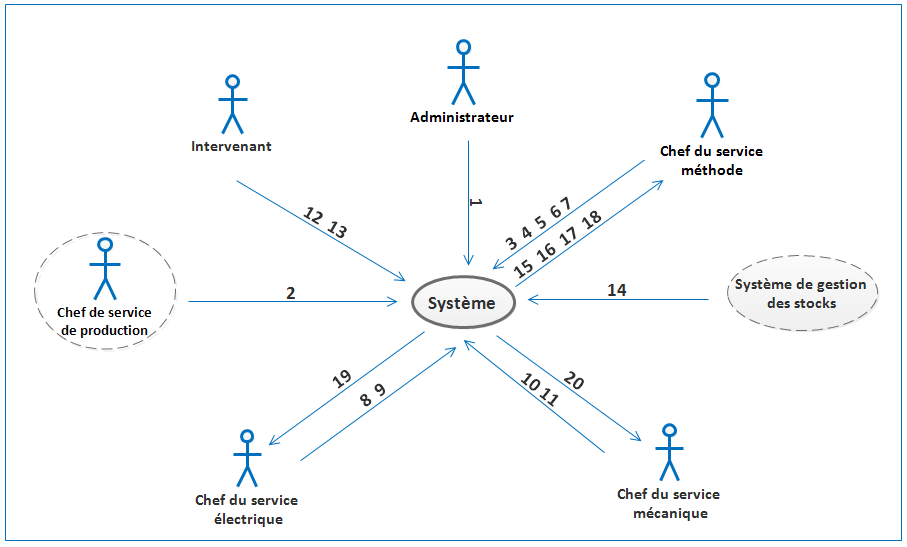
\includegraphics[width=0.9\linewidth]{./image_chapitre4/diagramme_contexte}
	\caption[Diagramme de contexte dynamique du nouveau syst�me]{Diagramme de contexte dynamique du nouveau syst�me.}
	\label{fig:diagramme du contexte}
\end{figure}
\newpage

\section{ Capture de besoins  }
\subsection{ Captures des besoins fonctionnels   }
La capture des besoins fonctionnels est la premi�re �tape de la branche gauche du cycle en Y. Elle formalise et d�taille ce qui a �t� �bauch� au cours de l'�tude pr�liminaire.\cite{ref08}\\[0.5\baselineskip]
Cette phase comporte :\cite{ref08}
\begin{itemize}
	\item L'identification des cas d'utilisation fonctionnels.
	\item La description textuelle des cas d'utilisation.
\end{itemize}
\subsubsection{ Identification des cas d'utilisations fonctionnels }
\textbf{D�finition}\\[0.5\baselineskip]
Un cas d'utilisation (use case) est un ensemble de s�quences d'actions r�alis�es par le syst�me et produisant un r�sultat observable int�ressant pour un acteur particulier. Un cas d'utilisation mod�lise un service rendu par le syst�me et exprime les interactions acteurs/syst�me. \cite{ref09}

\begin{figure}[H]
	\centering
	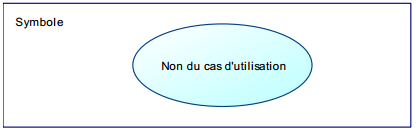
\includegraphics[width=0.9\linewidth]{./image_chapitre4/use_case}
	\caption[Repr�sentation d'un cas d'utilisation dans l'UML.]{Repr�sentation d'un cas d'utilisation dans l'UML.}
	\label{fig:use_case}
\end{figure}
Les cas d'utilisation sont une technique de capture des
besoins fonctionnels du syst�me. C'est une description "narrative" de comment est utilis� le syst�me.\cite{web11}\\[0.5\baselineskip]

\textbf{D�coupage modulaire des cas d'utilisations fonctionnels}\\[0.5\baselineskip]

Nous allons d�composer notre syst�me en modules avant d'identifier les cas d'utilisations fonctionnels. Par la suite nous allons d�tailler chaque module en une liste de cas d'utilisations en respectant la coh�rence fonctionnelle entre eux. \\[0.5\baselineskip]
Plus tard, chaque module sera repr�sent� par un package (paquetage).
Le tableau suivant repr�sente les modules de notre syst�me :
\newpage
\begin{center}
	\begin{tabular}{|p{5cm}|p{8cm}|}
		\hline
		\textbf{Num�ro du Module} &  \textbf{Titre }  \\
		\hline		
		\textbf{Module 1} & Gestion des �quipements\\
		\hline	
		\textbf{Module 2} & Gestion de la maintenance \\
		\hline		
		\textbf{Module 3} & Statistiques et ratios\\
		\hline	
	\end{tabular} \\
	\captionof{table}{D�coupage modulaire des cas d'utilisations fonctionnels en modules. }
	\label{tab19}
\end{center}

Dans ce qui suit, nous allons d�tailler chaque module en identifiant ses cas d'utilisations et en donnant leurs descriptions :\\

\textbf{Module1 : Gestion des �quipements}\\
\textbf{\small Liste des cas d'utilisations }\\
\begin{center}
	\begin{tabular}{|p{6cm}|p{8cm}|}
		\hline
		\textbf{Cas d'utilisation} &  \textbf{Acteurs }  \\
		\hline
		\textbf{G�rer la fiche technique de l'�quipement} & Chef du d�partement de gestion des �quipements\\
		\hline		
		\textbf{G�rer la nomenclature de l'�quipement} & Chef du d�partement de gestion des �quipements\\
		\hline	
		\textbf{G�rer la documentation de l'�quipement} & Chef du d�partement de gestion des �quipements\\
		\hline
		\textbf{G�rer les gammes de maintenance de l'�quipement } & Chef du d�partement de gestion des �quipements\\
		\hline		
	\end{tabular} \\
	\captionof{table}{liste des cas d'utilisations associ�s au module � Gestion des �quipements  �}
	\label{tab24}
\end{center}




\textbf{\small Diagramme des cas d'utilisations }\\
La figure suivante repr�sente le diagramme des cas d'utilisations du module � Gestion des �quipements  � :\\
\newpage
\begin{figure}[H]
	\centering
	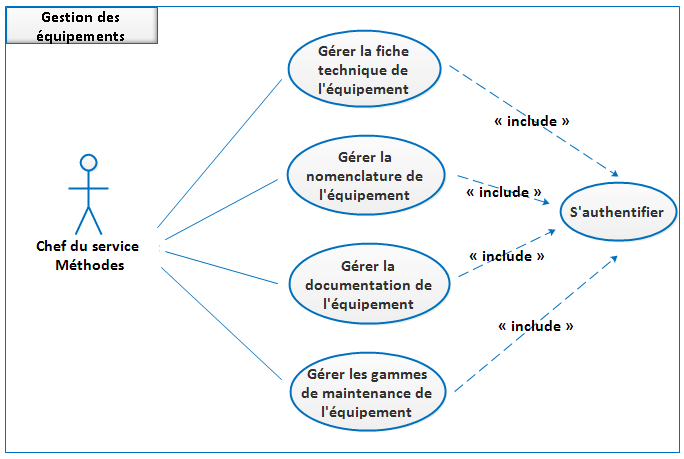
\includegraphics[width=0.9\linewidth]{./image_chapitre4/CUs_diagramme2}
	\caption[Diagramme des cas d'utilisations du module � Gestion des �quipements �]{Diagramme des cas d'utilisations du module � Gestion des �quipements : �}
	\label{fig:CUs_diagramme2}
\end{figure}
Dans ce qui suit, La description textuelle des diff�rents cas d'utilisations contenus dans le module � Gestion des �quipements �:\\[0.5\baselineskip]
\textbf{\footnotesize Description du cas � G�rer les documents  }

\begin{center}
	\begin{tabular}{|p{15cm}|}
		\hline
		\textbf{CU :  G�rer la fiche technique de l'�quipement}\\
		\hline	
		\textbf{Titre :}  G�rer la fiche technique de l'�quipement\\
		\hline
		\textbf{But :} Permet � l'utilisateur de cr�er/ modifier/ supprimer/ consulter la fiche technique d' un �quipement\\
		\hline
		\textbf{Acteur :}  Chef du d�partement de gestion des �quipements\\
		\hline
		\textbf{Pr�condition :}  L'utilisateur doit s'authentifier.\\
		\hline
		\textbf{Sc�nario nominal : } Ce cas commence lorsque l'utilisateur souhaite ex�cuter l'un des enchainements suivants : \\
		\textbf{Enchainement (a): }Cr�er une fiche technique  \\
		L'utilisateur acc�de au syst�me, il ajoute un nouvel �quipement en sp�cifiant ses informations ( code, d�signation, secteur ...etc.). \\
		 Si un ou plusieurs champs obligatoires sont vides ou invalides, l'exception s'ex�cute.  \\
		\textbf{Enchainement (b): }Modifier une fiche technique  \\
	L'utilisateur acc�de au syst�me, ce qui lui permet d'acc�der � la liste des �quipements, apr�s la s�lection d'un �quipement, il est possible de modifier un ou plusieurs champs.\\
	 Dans le cas d'une erreur dans la modification de la fiche technique, l'exception s'ex�cute. \\
	 \hline
\end{tabular} \\
\end{center}
\newpage
\begin{center}
 \begin{tabular}{|p{15cm}|}
     \hline
	 \textbf{Enchainement (c): }Supprimer une fiche technique  \\
	 L'utilisateur acc�de au syst�me, ce qui lui permet d'acc�der � la liste des �quipements, apr�s la s�lection d'un �quipement, il effectue une suppression logique .\\
		\textbf{Enchainement (d): }Consulter une fiche technique  \\
		L'utilisateur acc�de au syst�me, ce qui lui permet d'acc�der � la liste des �quipements, apr�s la s�lection d'un �quipement, il est possible de consulter la fiche technique de  � ce dernier.\\
		\hline	
		\textbf{Exception : }Le syst�me affiche un message d'erreur qui indique que les champs obligatoires ne sont pas correctement remplis. \\
		\hline	
		\textbf{Post condition : }  La cr�ation / modification/ suppression /consultation de la fiche technique d'un �quipement.\\
		\hline	
	\end{tabular} \\
	\captionof{table}{Description du cas � G�rer la fiche technique de l'�quipement   �}
	\label{tab25}
\end{center}


\textbf{\footnotesize Description du cas � G�rer la nomenclature de l'�quipement   }

\begin{center}
	\begin{tabular}{|p{15cm}|}
		\hline
		\textbf{CU :  G�rer la nomenclature de l'�quipement}\\
		\hline	
		\textbf{Titre :}  G�rer la nomenclature de l'�quipement\\
		\hline
		\textbf{But :} Permet � l'utilisateur de cr�er/ modifier/ supprimer/ consulter la nomenclature d'un �quipement\\
		\hline
		\textbf{Acteur :}  Chef du d�partement de gestion des �quipements\\
		\hline
		\textbf{Pr�condition :}  L'utilisateur doit s'authentifier.\\
		\hline
		\textbf{Sc�nario nominal : } Ce cas commence lorsque l'utilisateur souhaite ex�cuter l'un des enchainements suivants : \\
		\textbf{Enchainement (a): }Cr�er la nomenclature   \\
		L'utilisateur acc�de au syst�me, il s�lectionne un �quipement, puis il ajoute un ou plusieurs organes en remplissant un formulaire (d�signation, codification interne, rep�re, ...etc.). \\
		Si un ou plusieurs champs obligatoires sont vides ou invalides, l'exception s'ex�cute.  \\
		\textbf{Enchainement (b): }Modifier la nomenclature   \\
		L'utilisateur acc�de au syst�me, ce qui lui permet d'acc�der � la liste des �quipements, apr�s la s�lection d'un �quipement, il est possible de modifier un ou plusieurs organes.\\
		 Dans le cas d'une erreur dans la modification des organes, l'exception s'ex�cute. \\
		 \textbf{Enchainement (c): }Supprimer la nomenclature   \\
		 L'utilisateur acc�de au syst�me, ce qui lui permet d'acc�der � la liste des �quipements, apr�s la s�lection d'un �quipement, il est possible de supprimer des organes.\\
		\textbf{Enchainement (d): }Consulter la nomenclature   \\
		L'utilisateur acc�de au syst�me, ce qui lui permet d'acc�der � la liste des �quipements, apr�s la s�lection d'un �quipement, il est possible de consulter les organes de ce dernier.\\
		\hline	
		\textbf{Exception : } Le syst�me affiche un message d'erreur qui indique que les champs obligatoires ne sont pas correctement remplis. \\
		\hline
\end{tabular} \\
\end{center}
\newpage
\begin{center}
	\begin{tabular}{|p{15cm}|}
		\hline
		\textbf{Post condition : }  La cr�ation/ modification/ suppression/ consultation de la nomenclature d'un �quipement.\\
		\hline	
	\end{tabular} \\
	\captionof{table}{Description du cas � G�rer la nomenclature d'un  �quipement  �}
	\label{tab26}
\end{center}
\textbf{\footnotesize Description du cas � G�rer la documentation de l'�quipement   }

\begin{center}
	\begin{tabular}{|p{15cm}|}
		\hline
		\textbf{CU :  G�rer la documentation de l'�quipement}\\
		\hline	
		\textbf{Titre :}  G�rer la documentation de l'�quipement\\
		\hline
		\textbf{But :} Permet � l'utilisateur de cr�er/ modifier/ supprimer/ consulter la documentation d'un �quipement\\
		\hline
		\textbf{Acteur :}  Chef du d�partement de gestion des �quipements\\
		\hline
		\textbf{Pr�condition :}  L'utilisateur doit s'authentifier.\\
		\hline
		\textbf{Sc�nario nominal : } Ce cas commence lorsque l'utilisateur souhaite ex�cuter l'un des enchainements suivants : \\
		\textbf{Enchainement (a): }Cr�er la documentation   \\
		L'utilisateur acc�de au syst�me, il s�lectionne un �quipement, puis il ajoute un ou plusieurs documents en remplissant un formulaire (intitul�, type, contenu,  langue, ...etc.). \\
		Si un ou plusieurs champs obligatoires sont vides ou invalides, l'exception s'ex�cute.  \\
		\textbf{Enchainement (b): }Modifier la documentation   \\
		L'utilisateur acc�de au syst�me, ce qui lui permet d'acc�der � la liste des �quipements, apr�s la s�lection d'un �quipement, il est possible de modifier un ou plusieurs documents.\\
		Dans le cas d'une erreur dans la modification des documents, l'exception s'ex�cute. \\
		\textbf{Enchainement (c): }Supprimer la documentation   \\
		L'utilisateur acc�de au syst�me, ce qui lui permet d'acc�der � la liste des �quipements, apr�s la s�lection d'un �quipement, il est possible de supprimer des documents.\\
		\textbf{Enchainement (d): }Consulter la documentation   \\
		L'utilisateur acc�de au syst�me, ce qui lui permet d'acc�der � la liste des �quipements, apr�s la s�lection d'un �quipement, il est possible de consulter les documents de ce dernier.\\
		\hline	
		\textbf{Exception : } Le syst�me affiche un message d'erreur qui indique que les champs obligatoires ne sont pas correctement remplis. \\
		\hline
		\textbf{Post condition : }  La cr�ation/ modification/ suppression/ consultation de la documentation d'un �quipement.\\
		\hline	
	\end{tabular} \\
	\captionof{table}{Description du cas � G�rer la documentation d'un  �quipement �}
	\label{tab26}
\end{center}
\newpage
\textbf{\footnotesize G�rer les gammes de maintenance de l'�quipement  � }

\begin{center}
	\begin{tabular}{|p{15cm}|}
		\hline
		\textbf{CU :  G�rer les gammes de maintenance de l'�quipement  }\\
		\hline	
		\textbf{Titre :}  G�rer les gammes de maintenance de l'�quipement.\\
		\hline
		\textbf{But :} Permet � l'utilisateur de cr�er / modifier/ supprimer/ consulter une gamme de maintenance.\\
		\hline
		\textbf{Acteur :} Chef du d�partement de gestion des �quipements\\
		\hline
		\textbf{Pr�condition :}  L'utilisateur doit s'authentifier.\\
		\hline
		\textbf{Sc�nario nominal : } Ce cas commence lorsque l'utilisateur souhaite ex�cuter l'un des enchainements suivants : \\
		\textbf{Enchainement (a): }Cr�er une gamme   \\
		L'utilisateur acc�de au syst�me, il s�lectionne un �quipement, puis il ajoute une gamme (id\_gam, intitul�\_gam et periodicit�\_gam ), puis il cr�e le mode op�ratoire. \\
		Si un ou plusieurs champs obligatoires sont vides ou invalides, l'exception s'ex�cute.  \\
		\textbf{Enchainement (b): }Modifier une gamme   \\
		L'utilisateur acc�de au syst�me, ce qui lui permet d'acc�der � la liste des �quipements. Apr�s la s�lection d'un �quipement, il choisit une gamme et il effectue les modifications qu'il veut apporter. \\
		Dans le cas d'une erreur dans la modification d'une gamme, l'exception s'ex�cute. \\
		\textbf{Enchainement (c): }Supprimer une gamme   \\
		L'utilisateur acc�de au syst�me, ce qui lui permet d'acc�der � la liste des �quipements. Apr�s la s�lection d'un �quipement, il choisit une gamme et il la supprime. \\
		\textbf{Enchainement (d): }Consulter une gamme   \\
		L'utilisateur acc�de au syst�me, ce qui lui permet d'acc�der � la liste des �quipements. Apr�s la s�lection d'un �quipement, il choisit une gamme et il affiche les informations relatives � cette derni�re.\\
		\hline	
		\textbf{Exception : } Le syst�me affiche un message d'erreur qui indique que les champs obligatoires ne sont pas correctement remplis. \\
		\hline
		\textbf{Post condition : }  L'ajout/ modification/ suppression/ consultation d'une gamme de maintenance.\\
		\hline		
	\end{tabular} \\
	\captionof{table}{Description du cas � G�rer les gammes de maintenance de l'�quipement �}
	\label{tab29}
\end{center}
\newpage

\textbf{Module2 : Gestion de la maintenance}\\
\textbf{\small Liste des cas d'utilisations }\\
\begin{center}
	\begin{tabular}{|p{6cm}|p{8cm}|}
		\hline
		\textbf{Cas d'utilisation} &  \textbf{Acteurs }  \\
		\hline
		\textbf{G�rer les demandes de r�paration (DR) } & Chef de service de production\\
		\hline		
		\textbf{G�rer les ordres de travail (OR)} & Chef de service m�thodes\\
		\hline
		\textbf{G�n�rer le PMP d'un �quipement} & Chef du d�partement de gestion des �quipements, chef du service m�thodes, chef du service �lectrique ou m�canique et l'intervenant\\
		\hline	
		\textbf{G�rer le planning pr�ventif des �quipements} & Chef du service m�thodes et le chef de service �lectrique ou m�canique\\
		\hline		
		\textbf{G�rer le dossier des travaux de sous-traitance} & Sous-directeur de la maintenance\\
		\hline
	\end{tabular} \\
	\captionof{table}{liste des cas d'utilisations associ�s au module � Gestion de la maintenance �}
	\label{tab31}
\end{center}

\textbf{\small Diagramme des cas d'utilisations }\\
La figure suivante repr�sente le diagramme des cas d'utilisations du module � Gestion de la maintenance � :

\begin{figure}[H]
	\centering
	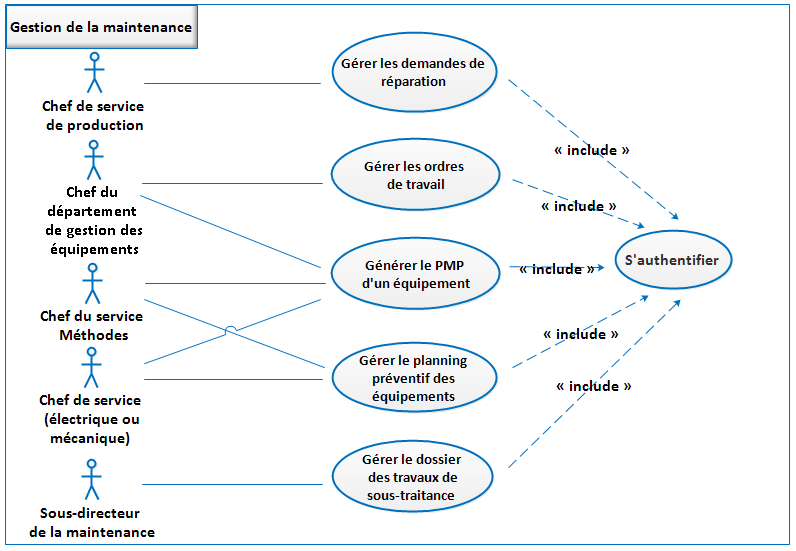
\includegraphics[width=0.9\linewidth]{./image_chapitre4/CUs_diagramme3}
	\caption[Diagramme des cas d'utilisations du module � Gestion de la maintenance curative �]{Diagramme des cas d'utilisations du module � Gestion de la maintenance �}
	\label{fig:CUs_diagramme3}
\end{figure}
Dans ce qui suit, La description textuelle des diff�rents cas d'utilisations contenus dans le module � Gestion de la maintenance � : \\[0.5\baselineskip]

\textbf{\footnotesize Description du cas � G�rer les demandes de r�paration   }

\begin{center}
	\begin{tabular}{|p{15cm}|}
		\hline
		\textbf{CU : G�rer les demandes de r�paration (DR)   }\\
		\hline	
		\textbf{Titre :}  G�rer les demandes de r�paration.\\
		\hline
		\textbf{But :} Permet � l'utilisateur de cr�er/ modifier/ /supprimer/ consulter une  demande de r�paration.\\
		\hline
		\textbf{Acteur :} Chef du service de production.\\
		\hline
		\textbf{Pr�condition :}  L'utilisateur doit s'authentifier.\\
		\hline
		\textbf{Sc�nario nominal : } Ce cas commence lorsque l'utilisateur souhaite ex�cuter l'un des enchainements suivants : \\	
		\textbf{Enchainement (a): } Cr�er une demande de r�paration      \\
		L'utilisateur s�lectionne � �tablir une demande de r�paration �, puis il saisit les informations de cette derni�re (id, date, d�tail de la panne , ...etc.). Si un ou plusieurs champs obligatoires sont vides ou invalides, l'exception s'ex�cute.\\
		Dans le cas d'une maintenance pr�ventive, la demande de r�paration est cr��e automatiquement par syst�me. \\
		\textbf{Enchainement (b): } Modifier une demande de r�paration      \\
		L'utilisateur s�lectionne une demande de r�paration qu'il a �tablie, puis il met � jour les informations de cette derni�re. \\
		Si un ou plusieurs champs obligatoires sont vides ou invalides, l'exception s'ex�cute.  \\
		\textbf{Enchainement (c): } Supprimer une demande de r�paration      \\
		L'utilisateur s�lectionne une demande de r�paration qu'il a �tablie, puis il la supprime. \\
		\textbf{Enchainement (d): } Consulter une demande de r�paration     \\
		L'utilisateur recherche une demande de r�paration, une fois trouv�e, il consulte les informations de cette derni�re et il peut aussi suivre son �tat qui peut �tre en attente, valid�e ou annul�e.\\
		\hline
		\textbf{Exception : } Le syst�me affiche un message d'erreur qui indique que les champs obligatoires ne sont pas correctement remplis. \\
		\hline
		\textbf{Post condition : }  La cr�ation/ modification/ suppression/ consultation d'une demande de r�paration.\\
		\hline		
	\end{tabular} \\
	\captionof{table}{Description du cas � G�rer les demandes de r�paration       �}
	\label{tab32}
\end{center}

\newpage
\textbf{\footnotesize Description du cas � G�rer les ordres de travail }

\begin{center}
	\begin{tabular}{|p{15cm}|}
		\hline
		\textbf{CU : G�rer les ordres de travail (OT)  }\\
		\hline	
		\textbf{Titre :}  G�rer les ordres de travail .\\
		\hline
		\textbf{But :} Permet � l'utilisateur de cr�er/ modifier/ supprimer/ consulter un ordre de travail.\\
		\hline
		\textbf{Acteur (cr�er/ modifier/ supprimer) :}  Le chef du service m�thodes.\\
		\textbf{Acteur (consulter) :}  chef de service �lectrique ou m�canique et l'intervenant.\\
		\hline
		\textbf{Pr�condition :}  L'utilisateur doit s'authentifier.\\
		\hline
		\textbf{Sc�nario nominal : } Ce cas commence lorsque l'utilisateur souhaite ex�cuter l'un des enchainements suivants : \\	
		\textbf{Enchainement (a): } Cr�er un ordre de travail      \\
		L'utilisateur s�lectionne une demande de r�paration, puis il saisit les informations relatives � l'ordre de travail � savoir : id, date, description des travaux, date d�but pr�vue, date fin pr�vue, ...etc.\\
		Si un ou plusieurs champs obligatoires sont vides ou invalides, l'exception s'ex�cute. \\
		\textbf{Enchainement (b): } Modifier un ordre de travail      \\
		L'utilisateur s�lectionne un ordre de travail, puis il met � jour les informations de ce dernier.\\ Si un ou plusieurs champs obligatoires sont vides ou invalides, l'exception s'ex�cute.  \\
		\textbf{Enchainement (c): } supprimer un ordre de travail \\
		L'utilisateur s�lectionne un ordre de travail, puis il le supprime.\\ 
		\textbf{Enchainement (d): } consulter un ordre de travail \\
		L'utilisateur s�lectionne un ordre de travail, puis il consulte les informations de ce dernier.\\
		\textbf{Exception : } Le syst�me affiche un message d'erreur qui indique que les champs obligatoires ne sont pas correctement remplis. \\
		\hline
		\textbf{Post condition : }  La cr�ation/ modification/ suppression / consultation d'un ordre de travail.\\
		\hline		
	\end{tabular} \\
	\captionof{table}{Description du cas � G�rer les ordres de travail �}
	\label{tab33}
\end{center}

\textbf{\footnotesize Description du cas � G�n�rer le PMP d'un �quipement �   }

\begin{center}
	\begin{tabular}{|p{15cm}|}
		\hline
		\textbf{CU : G�n�rer le PMP d'un �quipement automatiquement     }\\
		\hline	
		\textbf{Titre :}  G�n�rer le PMP ( Plan de Maintenance Pr�ventive ) d'un �quipement automatiquement.\\
		\hline
		\textbf{But :} Permet � l'utilisateur de consulter le PMP d'un �quipement qui est cr�� automatiquement par le syst�me.\\
		\hline
		\textbf{Acteur (consulter)  :} chef du d�partement de gestion des �quipements, chef du service m�thodes, chef du service �lectrique ou m�canique et l'intervenant.\\
		\hline
		\textbf{Pr�condition :}  L'utilisateur doit s'authentifier et au moins une gamme de maintenance doit exister au pr�alable.\\
		\hline
\end{tabular} \\
\end{center}
\newpage
\begin{center}
	\begin{tabular}{|p{15cm}|}
		\hline
		\textbf{Sc�nario nominal : } Ce cas commence lorsque l'utilisateur souhaite consulter le PMP d'un �quipement. \\	
		\textbf{Enchainement : } Consulter le PMP d'un �quipement \\
		L'utilisateur acc�de au syst�me, puis il choisit un �quipement pour lequel il veut consulter le PMP. Le syst�me affiche les informations de ce dernier (les op�rations pr�ventives pr�vues, observations, ...etc.) \\
		S'il n'existe pas au moins une gamme de maintenance �tablie concernant l'�quipement, l'exception s'ex�cute.\\
		\hline
		\textbf{Exception : } Le syst�me affiche un message d'erreur qui indique qu'aucune gamme de maintenance n'a �t� cr��e.\\
		\hline
		\textbf{Post condition : }  La consultation du PMP d'un �quipement.\\
		\hline		
	\end{tabular} \\
	\captionof{table}{Description du cas � G�n�rer le PMP d'un �quipement �}
	\label{tab36}
\end{center}

\textbf{\footnotesize Description du cas � G�rer le planning pr�ventif des �quipements �   }

\begin{center}
	\begin{tabular}{|p{15cm}|}
		\hline
		\textbf{CU : G�rer le planning pr�ventif des �quipements     }\\
		\hline	
		\textbf{Titre :}  G�rer le planning pr�ventif des �quipements  qui est cr�� automatiquement par le syst�me.\\
		\hline
		\textbf{But :} Permet � l'utilisateur de modifier/ consulter le planning pr�ventif des �quipements.\\
		\hline
		\textbf{Acteur (modifier)  :}  Le chef du service m�thodes et le chef du service �lectrique ou m�canique.\\
		\textbf{Acteur (consulter) :} Le chef du service m�thodes, chef du service �lectrique ou m�canique et l'intervenant.\\
		\hline
		\textbf{Pr�condition :}  L'utilisateur doit s'authentifier et les gammes de maintenance doivent �tre enregistr�es au pr�alable..\\
		\hline
		\textbf{Sc�nario nominal : } Ce cas commence lorsque l'utilisateur souhaite ex�cuter l'un des enchainements suivants : \\	
		\hline
		\textbf{Enchainement (a): } Modifier le planning pr�ventif des �quipements      \\
		L'utilisateur acc�de au syst�me, il s�lectionne un planning et apporte des modification qu'il veut ( taches, intervenant, ...etc.).  
		Si un ou plusieurs champs obligatoires sont vides ou invalides, l'exception 1 s'ex�cute. \\
		\textbf{Enchainement (b): } Consulter le planning pr�ventif des �quipements     \\
		L'utilisateur acc�de au syst�me, il recherche un planning pr�ventif des �quipements et il visualise les  informations relatives �� ce dernier.\\
		S'il n'existe pas au moins une gamme de maintenance, l'exception 2 s'ex�cute.\\
		\hline
		\textbf{Exception 1 : } Le syst�me affiche un message d'erreur qui indique que les champs obligatoires ne sont pas correctement remplis. \\
		\hline
\end{tabular} \\
\end{center}
\newpage
\begin{center}
	\begin{tabular}{|p{15cm}|}
		\hline
		\textbf{Exception 2 : } Le syst�me affiche un message d'erreur qui indique qu'aucune gamme de maintenance n'a �t� cr��e.\\
		\hline
		\textbf{Post condition : }  La modification/ consultation du planning pr�ventif des �quipements.\\
		\hline		
	\end{tabular} \\
	\captionof{table}{Description du cas � G�rer le planning pr�ventif des �quipements  �}
	\label{tab36}
\end{center}


\textbf{\footnotesize Description du cas � G�rer le dossier des travaux de sous-traitance     }

\begin{center}
	\begin{tabular}{|p{15cm}|}
		\hline
		\textbf{CU : G�rer le dossier des travaux de  sous-traitance     }\\
		\hline	
		\textbf{Titre :}  G�rer le dossier des travaux de sous-traitance  .\\
		\hline
		\textbf{But :} Permet � l'utilisateur de cr�er/ modifier/ supprimer/ consulter un dossier des travaux de sous-traitance.\\
		\hline
		\textbf{Acteur :}  Sous-directeur de la maintenance.\\
		\hline
		\textbf{Pr�condition :}  L'utilisateur doit s'authentifier. \\
		\hline
		\textbf{Sc�nario nominal : } Ce cas commence lorsque l'utilisateur souhaite ex�cuter l'un des enchainements suivants : \\	
		\textbf{Enchainement (a): } Cr�er un dossier des travaux de sous-traitance      \\
		L'utilisateur acc�de au syst�me, il cr�e un dossier des travaux sous-trait�s, il saisit les informations concernant de ces derniers (le sous-traitant, les interventions r�alis�es par ce dernier,...etc.). Il proc�de ensuite au scan du contrat de sous-traitance version papier puis il met la version �lectronique dans le dossier. \\
		Si un ou plusieurs champs obligatoires sont vides ou invalides, l'exception s'ex�cute.\\
		\textbf{Enchainement (b): } Modifier un dossier des travaux de sous-traitance      \\
		L'utilisateur acc�de au syst�me, ce qui lui permet d'acc�der � la liste des dossiers de travaux sous-trait�s, ensuite il peut s�lectionner un dossier et effectuer les modifications qu'il souhaite concernant ses informations.\\
		 Si un ou plusieurs champs obligatoires sont vides ou invalides, l'exception s'ex�cute.  \\
		 \textbf{Enchainement (c): } Supprimer un dossier des travaux de sous-traitance      \\
		 L'utilisateur acc�de au syst�me, ce qui lui permet d'acc�der � la liste des dossiers de travaux sous-trait�s, ensuite il peut s�lectionner un dossier et il le supprime.\\
		\textbf{Enchainement (d): } Consulter un dossier des travaux de sous-traitance     \\
		L'utilisateur acc�de au syst�me, ce qui lui permet d'acc�der � la liste des dossiers de travaux sous-trait�s, ensuite il peut s�lectionner un dossier et visualiser ses informations.\\
		\hline
		\textbf{Exception : } Le syst�me affiche un message d'erreur qui indique que les champs obligatoires ne sont pas correctement remplis. \\
		\hline
		\textbf{Post condition : }  La cr�ation/ modification/ suppression/ consultation du dossier des travaux de sous-traitance.\\
		\hline		
	\end{tabular} \\
	\captionof{table}{Description du cas � G�rer le dossier des travaux de  sous-traitance  �}
	\label{tab34}
\end{center}
\newpage

\textbf{Module3 : Statistiques et ratios}\\
\textbf{\small Liste des cas d'utilisations }\\
\begin{center}
	\begin{tabular}{|p{6cm}|p{8cm}|}
		\hline
		\textbf{Cas d'utilisation} &  \textbf{Acteurs }  \\
		\hline
		\textbf{G�n�rer les statistiques et les ratios } & Sous-directeur de la maintenance, chef du d�partement de gestion des �quipements, chef du service m�thodes, chef du service �lectrique ou m�canique \\
		\hline		
	\end{tabular} \\
	\captionof{table}{cas d'utilisations associ�s au module � Statistiques et ratios �}
	\label{tab31}
\end{center}

\textbf{\small Diagramme des cas d'utilisations }\\
La figure suivante repr�sente le diagramme des cas d'utilisations du module � Statistiques et ratios � :

\begin{figure}[H]
	\centering
	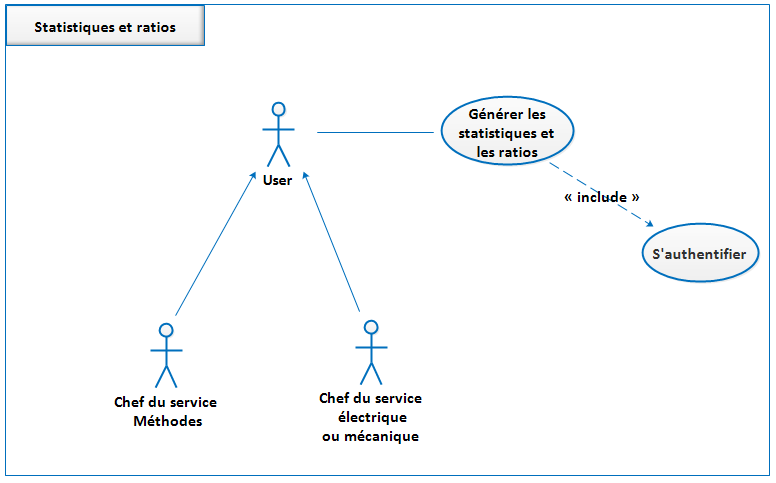
\includegraphics[width=0.9\linewidth]{./image_chapitre4/CUs_diagramme5}
	\caption[Diagramme des cas d'utilisations du module � Statistiques et les ratios �]{Diagramme des cas d'utilisations du module � Statistiques et ratios �}
	\label{fig:CUs_diagramme3}
\end{figure}

Dans ce qui suit, La description textuelle du cas d'utilisation contenu dans le module � Statistiques et ratios  �: \\[0.5\baselineskip]
\newpage
\textbf{\footnotesize Description du cas � G�n�rer les statistiques et les ratios   �   }

\begin{center}
	\begin{tabular}{|p{15cm}|}
		\hline
		\textbf{CU : G�n�rer les statistiques et les ratios      }\\
		\hline	
		\textbf{Titre :}  G�n�rer les statistiques et les ratios concernant la maintenance   .\\
		\hline
		\textbf{But :} Permet � l'utilisateur de consulter les statistiques et les ratios sur la maintenance.\\
		\hline
		\textbf{Acteur :}  Sous-directeur de la maintenance, chef du d�partement de gestion des �quipements, chef du service m�thodes, chef du service �lectrique ou m�canique.\\
		\hline
		\textbf{Pr�condition :}  L'utilisateur doit s'authentifier.\\
		\hline
		\textbf{Sc�nario nominal : } Ce cas commence lorsque l'utilisateur souhaite consulter les statistiques et les ratios. \\	
		\textbf{Enchainement : }      \\
		L'utilisateur acc�de au syst�me, il est possible qu'il consulte les statistiques et les ratios concernant la maintenance en choisissant des param�tres (service, date, ...etc.).\\
		 Dans le cas o� les statistiques ne sont pas disponibles, l'exception s'ex�cute.\\
		\hline
       \textbf{Exception : } Le syst�me affiche un message d'erreur qui indique que les les statistiques et les ratios ne sont pas disponibles . \\
       \hline
       \textbf{Post condition : }  La consultation des statistiques et des ratios.\\
       \hline		
    \end{tabular} \\
    \captionof{table}{Description du cas � G�n�rer les statistiques et les ratios   �}
    \label{tab37}
\end{center}


\subsection{ Captures des besoins techniques   }
Nous avons pr�c�demment identifi� les besoins fonctionnels qui repr�sentent la branche gauche (la branche fonctionnelle) de la m�thode � 2TUP �. Dans cette partie, nous allons nous pencher � identifier les besoins techniques.\\[0.5\baselineskip]
Cette �tape repr�sente la branche droite de la d�marche 2TUP, elle consiste � d�terminer tous les �l�ments n�cessaires pour une architecture appropri�e � la conception du syst�me. Elle nous permet ainsi de conna�tre le mat�riel, � savoir les machines et r�seaux, les progiciels � int�grer, ainsi que les outils retenus pour le d�veloppement. \cite{ref08}\\[0.5\baselineskip]

� La capture des besoins techniques couvre, par compl�mentarit� avec celle des besoins fonctionnels, toutes les contraintes qui ne traitent ni de la description du m�tier des utilisateurs, ni de la description applicative. �. \cite{ref08}.\\[0.5\baselineskip]

Pour la capture des besoins techniques, nous avons proc�d� comme suit :

\begin{itemize}
	\item Sp�cifications techniques du point de vue mat�riel.
	\item Sp�cifications techniques du point de vue logiciel.
	\item Identification des exploitants du syst�me.
	\item Identification des cas d'utilisation.
\end{itemize}

\subsubsection{ Sp�cifications techniques du point de vue mat�riel  }
La sp�cification technique du point de vue mat�riel consiste � traiter les contraintes relatives � la configuration du r�seau mat�riel. Ces contraintes sont de nature g�ographique, organisationnelle et technique. Elles concernent les performances d'acc�s aux donn�es, la s�curit� du syst�me, le mode d'utilisation du syst�me, ... etc. \cite{ref08}.\\

Dans cette partie, nous allons pr�senter la configuration choisie pour notre syst�me et qui est l'architecture 3 niveaux (3-tiers).\\

Le principe d'une architecture 3-tiers consiste � s�parer la r�alisation des trois parties (stockage des donn�es, logique applicative, pr�sentation). Les �l�ments permettant la r�alisation classique d'un syst�me en architecture trois tiers sont les suivants : \cite{web12}.\\
\begin{itemize}
	\item Navigateur web (client), c'est l'ordinateur demandeur de ressources, �quip�e d'une interface utilisateur qui repr�sente la partie visible de l'application et qui est charg�e de la pr�sentation.
	\item Serveur applicatif (middleware), charg� de la mod�lisation des processus m�tiers et la validation des donn�es.
	\item Syst�me de base de donn�es pour le stockage des donn�es.
\end{itemize}

\begin{figure}[H]
	\centering
	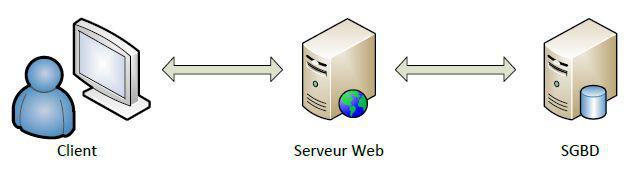
\includegraphics[width=0.9\linewidth]{./image_chapitre4/web_3tiers}
	\caption[Architecture � 3 niveaux] {Architecture � 3 niveaux}
	\label{fig:web_3tiers}
\end{figure}

Nous avons opt� pour ce type d'architectures pour les avantages que nous allons pr�senter ci-dessous :\\

\begin{itemize}
	\item Ne n�cessite pas assez de temps pour la mise en \oe uvre (r�alisable en court terme).
	\item 	La modification et la mise � jour des composantes de l'application sont tr�s faciles et cela permet une �volution r�guli�re du syst�me.
	\item Am�lioration de la s�curit� (acc�s � la base n'est effectu� que par le serveur).
	\item De meilleures performances, �tant donn� le partage des t�ches entre les diff�rents
	serveurs.
	\item D'un point de vue d�veloppement, la s�paration qui existe entre le client, le serveur et le SGBD permet une sp�cialisation des d�veloppeurs sur chaque tiers de l'architecture.
\end{itemize}

\subsubsection{ Sp�cifications techniques du point de vue logiciel  }
\begin{itemize}
	\item Langage de programmation : PHP 5.6.16.
	\item 	Framework : Laravel 5.1.
	\item Syst�me de gestion des bases de donn�es : MySQL 5.6.17.
	\item Serveur d'application : Serveur Apache 2.4.17.
	\item Environnement de d�veloppement : WAMPSERVER 2.5.
\end{itemize}

\subsubsection{ Identification des exploitants du syst�me   }
\textbf{D�finition}\\
L'exploitant est un acteur au sens d'UML, s'il ne b�n�ficie que des fonctionnalit�s techniques du syst�me. � \cite{ref08}.\\[0.5\baselineskip]

Pour notre cas les exploitants du syst�me sont :
\begin{itemize}
	\item \textbf{L'administrateur :} charg� de g�rer l'ensemble des utilisateurs du syst�me : cr�er ces utilisateurs et de leur attribuer les droits d'acc�s.
	\item \textbf{L'utilisateur :} celui qui utilise une des fonctionnalit�s du syst�me.
	
\end{itemize}

\subsubsection{  Identification des cas d'utilisation   }
Dans ce qui suit, nous allons d�tailler le module qui contient les cas d'utilisations techniques en donnant leurs descriptions :\\

\textbf{\small Liste des cas d'utilisations }\\
\begin{center}
	\begin{tabular}{|p{6cm}|p{8cm}|}
		\hline
		\textbf{Cas d'utilisation} &  \textbf{Acteurs }  \\
		\hline
		\textbf{G�rer l'authentification} & Tous les utilisateurs du syst�me\\
		\hline		
		\textbf{G�rer les profils utilisateurs} & Administrateur\\
		\hline	
		\textbf{G�rer les utilisateurs} & Administrateur\\
		\hline		
	\end{tabular} \\
	\captionof{table}{liste des cas d'utilisations techniques}
	\label{tab20}
\end{center}
\textbf{\small Diagramme des cas d'utilisations }\\
La figure suivante repr�sente le diagramme des cas d'utilisations techniques  :\\
\newpage

\begin{figure}[H]
	\centering
	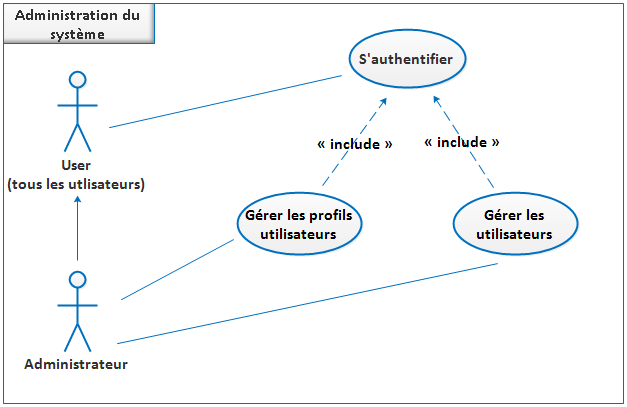
\includegraphics[width=0.9\linewidth]{./image_chapitre4/CUs_diagramme1}
	\caption[Diagramme des cas d'utilisations techniques ]{Diagramme des cas d'utilisations techniques}
	\label{fig:CUs_diagramme1}
\end{figure}
Dans ce qui suit, La description textuelle des diff�rents cas d'utilisations techniques : \\[0.5\baselineskip]
\textbf{\footnotesize Description du cas � G�rer l'authentification  }
\begin{center}
	\begin{tabular}{|p{15cm}|}
		\hline
		\textbf{CU : G�rer l'authentification}\\
		\hline	
		\textbf{Titre:} G�rer l'authentification d'un utilisateur\\
		\hline
		\textbf{But:} Permet � l'utilisateur de se connecter\\
		\hline
		\textbf{Acteur:}  Tous les utilisateurs du syst�me\\
		\hline
		\textbf{Pr�condition:}  L'utilisateur doit disposer d'un compte et des droits d'acc�s au syst�me.\\
		\hline
		\textbf{Sc�nario nominal : } Ce cas commence lorsque l'utilisateur souhaite se connecter � l'application. \\
		\textbf{Enchainement : }
		Une fois l'application lanc�e sur le navigateur web, l'utilisateur acc�de � une fen�tre de login, ce qui lui permet de saisir son nom d'utilisateur et son mot de passe. Le syst�me v�rifie les informations saisies par l'utilisateur en les comparants avec les donn�es enregistr�es sur la base de donn�es.\\
		Dans le cas o� les informations ne correspondent pas aux informations enregistr�es l'exception est ex�cut�e.\\
		\hline	
		\textbf{Exception : }  Le syst�me affiche un message d'erreur qui indique que les informations saisies sont erron�es.\\
		\hline
		\textbf{Post condition : }  L'utilisateur se connecte au syst�me et acc�de aux privil�ges correspondants � son profil.\\
		\hline	
	\end{tabular} \\
	\captionof{table}{Description du cas � G�rer l'authentification �}
	\label{tab21}
\end{center}
\newpage
\textbf{\footnotesize Description du cas � G�rer les profils utilisateurs �  }
\begin{center}
	\begin{tabular}{|p{15cm}|}
		\hline
		\textbf{CU :  G�rer les profils utilisateurs}\\
		\hline	
		\textbf{Titre :}  G�rer les profils utilisateurs\\
		\hline
		\textbf{But :} Permet d'ajouter/ modifier/ supprimer/ consulter un profil utilisateur\\
		\hline
		\textbf{Acteur :}  Administrateur\\
		\hline
		\textbf{Pr�condition :}  l'utilisateur doit d'abord s'authentifier.\\
		\hline
		\textbf{Sc�nario nominal : } Ce cas commence lorsque l'administrateur souhaite ex�cuter l'un des enchainements suivants : \\
		\textbf{Enchainement (a): }Ajouter un profil utilisateur \\
		L'administrateur ins�re un profil en sp�cifiant son intitul� et en lui affectant des privil�ges.\\
		Si un ou plusieurs champs obligatoires sont vides ou invalides, l'exception s'ex�cute.\\
		\textbf{Enchainement (b): }Modifier un profil utilisateur \\
		L'administrateur affiche la liste des profils utilisateur et s�lectionne celui qu'il souhaite modifier, et enfin met � jour les donn�es le concernant.\\
		Si un ou plusieurs champs obligatoires sont vides ou invalides lors de la modification, l'exception s'ex�cute.\\
		\textbf{Enchainement (c): }Supprimer  un profil utilisateur \\
		L'administrateur affiche la liste des profils utilisateur, une fois le profil s�lectionn�, il supprime logiquement les informations et les privil�ges de ce dernier.\\
		\textbf{Enchainement (d): }Consulter un profil utilisateur \\
		L'administrateur affiche la liste des profils utilisateur, apr�s la s�lection de celui qu'il souhaite consulter, il peut visualiser toutes ses informations (intitul�, privil�ge, ...etc).\\
		\hline	
		\textbf{Exception : }  Le syst�me affiche un message d'erreur qui indique que les champs obligatoires n'e sont pas correctement remplis.\\
		\hline
		\textbf{Post condition : }  La cr�ation/ modification/ suppression/ consultation d'un profil utilisateur.\\
		\hline	
	\end{tabular} \\
	\captionof{table}{Description du cas � G�rer les profils utilisateurs  �}
	\label{tab22}
\end{center}

\textbf{\footnotesize Description du cas � G�rer les utilisateurs  }

\begin{center}
	\begin{tabular}{|p{15cm}|}
		\hline
		\textbf{ CU :  G�rer les utilisateurs}\\
		\hline	
		\textbf{Titre :}  G�rer les utilisateurs\\
		\hline
		\textbf{But :} Permet d'ajouter/ modifier/ supprimer/ consulter un profil utilisateur\\
		\hline
		\textbf{Acteur :}  Administrateur\\
		\hline
		\textbf{Pr�condition :}  l'utilisateur doit d'abord s'authentifier.\\
		\hline
		\textbf{Sc�nario nominal : } Ce cas commence lorsque l'administrateur souhaite ex�cuter l'un des enchainements suivants : \\
		\hline
		
    \end{tabular} \\
\end{center}
\newpage
\begin{center}
	\begin{tabular}{|p{15cm}|}
		\hline
		\textbf{Enchainement (a): }Ajouter un utilisateur \\
		L'administrateur ajoute un utilisateur en saisissant ces informations (nom d'utilisateur, mot de passe, ...etc.), il effectue son enregistrement dans la base de donn�es, dans le cas d'une erreur dans un champ l'exception s'ex�cute.\\
		\textbf{Enchainement (b): }Modifier un utilisateur \\
		L'administrateur consulte la liste des utilisateurs, une fois l'utilisateur s�lectionn�, il acc�de � ses informations et proc�de � la mise � jour de ces derni�res.\\
		Dans le cas d'une erreur dans un champ l'exception s'ex�cute.\\
		\textbf{Enchainement (c): }Supprimer  un utilisateur \\
		L'administrateur consulte la liste des utilisateurs, une fois l'utilisateur s�lectionn�, il supprime logiquement les informations et les privil�ges de ce dernier.\\
		\textbf{Enchainement (d): }Consulter un utilisateur \\
		L'administrateur affiche la liste des utilisateur, apr�s la s�lection de celui qu'il souhaite consulter, il peut visualiser toutes ses informations (nom, pr�nom, nom d'utilisateur, ...etc.).\\
		\hline	
		\textbf{Exception : }  Le syst�me affiche un message d'erreur qui indique que les champs obligatoires ne sont pas correctement remplis.\\
		\hline
		\textbf{Post condition : }  La cr�ation/ modification/ suppression/ consultation d'un utilisateur.\\
		\hline	
	\end{tabular} \\
	\captionof{table}{Description du cas � G�rer les utilisateurs  �}
	\label{tab23}
\end{center}



\newpage
\section{ Analyse  }

L'analyse est la phase qui consiste � clarifier les besoins des utilisateurs du syst�me d'une mani�re
d�taill�e.\\[0.5\baselineskip]
Cette phase comporte:\cite{ref08}
\begin{itemize}
	\item D�coupage en cat�gories.
	\item D�veloppement du mod�le statique.
	\item D�veloppement du mod�le dynamique.
\end{itemize}

\subsection{ D�coupage en cat�gories  }


Cette phase constitue la premi�re �tape de l'analyse du syst�me. La d�marche
mise en \oe uvre consiste � utiliser la notion de package pour d�finir les cat�gories.\\[0.5\baselineskip]
Le d�coupage en cat�gories se base essentiellement sur deux principes qui
sont : les classes et les cat�gories. \cite{ref08}.\\
Cette activit� va s'affiner de mani�re it�rative au cours du
d�veloppement du projet. Elle se situe sur la branche gauche du cycle en Y et succ�de � la
capture des besoins fonctionnels.\\[0.5\baselineskip]
Une cat�gorie consiste en un regroupement logique de classes � forte coh�rence interne et
faible couplage externe. \cite{ref08}\\[0.5\baselineskip]

\begin{figure}[H]
	\centering
	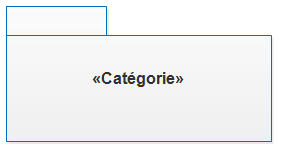
\includegraphics[width=0.5\linewidth]{./image_chapitre4/Categorie}
	\caption[Repr�sentation d'une cat�gorie des classes dans l'UML.]{Repr�sentation d'une cat�gorie des classes dans l'UML.}
	\label{fig:cat�gorie}
\end{figure}


Le d�coupage en cat�gories de notre projet a donn� le r�sultat suivant :

\begin{center}
	\begin{tabular}{|p{6cm}|p{8.5cm}|}
		\hline
		\textbf{Paquage} &  \textbf{Cas d'utilisation }  \\
		\hline
		\multirow{3}{*}{Administration du syt�me} & G�rer l'authentification  \\ \cline{2-2} 
		&  G�rer les profils utilisateurs \\ \cline{2-2} 
		& G�rer les utilisateurs \\ 
		\hline
	\end{tabular} \\
\end{center}
\newpage
\begin{center}
	\begin{tabular}{|p{6cm}|p{8.5cm}|}
		\hline
		\multirow{4}{*}{Gestion des �quipements} & G�rer la fiche technique de l'�quipement  \\ \cline{2-2} 
		&  G�rer la nomenclature de l'�quipement \\ \cline{2-2} 
		&  G�rer la documentation de l'�quipement \\ \cline{2-2} 
		&  G�rer les gammes de maintenance de l'�quipement \\  
		\hline
		\multirow{5}{*}{Gestion de la maintenance} & G�rer les demandes de r�paration (DR)  \\ \cline{2-2} 
		&  G�rer les ordres de travail (OR) \\ \cline{2-2} 
		&  G�n�rer le PMP d'un �quipement \\ \cline{2-2} 
		&  G�rer le planning pr�ventif des �quipements \\ \cline{2-2} 
		&  G�rer le dossier des travaux de sous-traitance \\
		\hline
		Statistiques et les ratios & G�n�rer les statistiques et les ratios\\
		\hline		
	\end{tabular} \\
	\captionof{table}{D�coupage en cat�gories}
	\label{tab38}
\end{center}

La figure suivante repr�sente le  d�coupage en cat�gories de notre syst�me sous UML :
\begin{figure}[H]
	\centering
	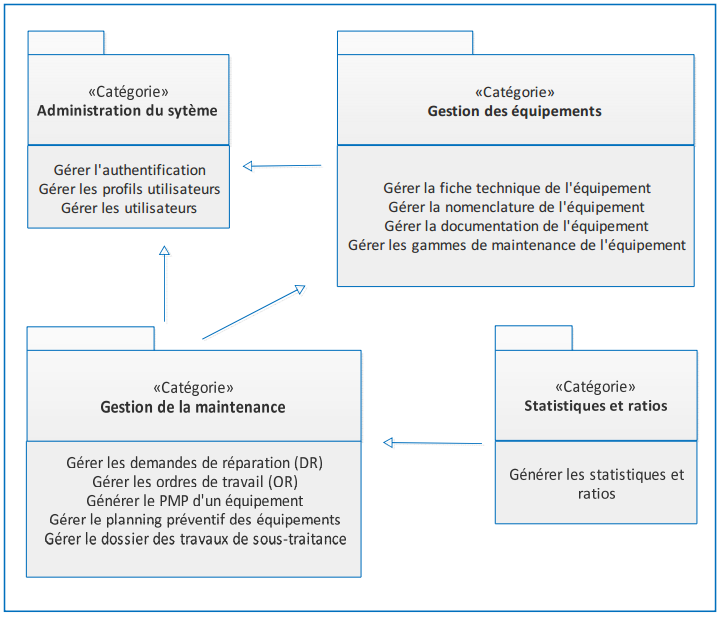
\includegraphics[width=0.9\linewidth]{./image_chapitre4/decoupage_categories}
	\caption[D�coupage en cat�gories en UML.]{D�coupage en cat�gories UML.}
	\label{fig:decpupage_categorie}
\end{figure}

\subsection{ D�veloppement du mod�le statique  }
Le d�veloppement du mod�le statique est la deuxi�me activit� de l'�tape d'analyse. Elle se situe
dans la branche gauche du cycle en Y et succ�de au d�coupage en cat�gories.\cite{ref08}.\\[0.5\baselineskip]
cette �tape consiste � d�tailler les classes, pr�alablement d�termin�es dans la capture des besoins, avec les attributs et les m�thodes correspondants.\\[0.5\baselineskip]
Une classe est l'abstraction d'un ensemble d'objets qui poss�dent une structure identique
(liste des attributs) et un m�me comportement (liste op�rations). \cite{ref09}\\[0.5\baselineskip]
Au cours de cette phase, nous allons associer � chaque cat�gorie un diagramme de classe.
\begin{figure}[H]
	\centering
	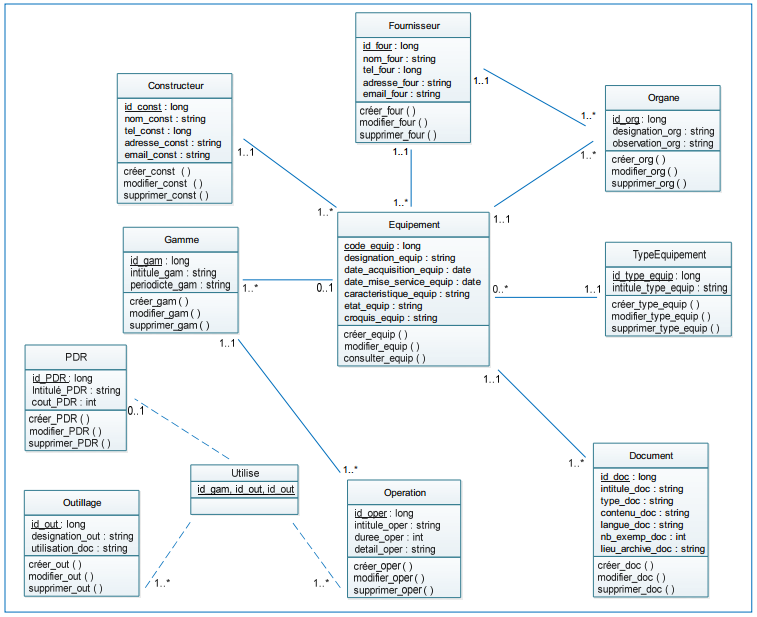
\includegraphics[width=1\linewidth]{./image_chapitre4/Diagramme_classes_documentation}
	\caption[Diagramme de classe correspondant � la cat�gorie  � Gestion de la documentation �.]{Diagramme de classe correspondant � la cat�gorie  � Gestion de la documentation �.}
	\label{fig:Diagramme_classes_documentation}
\end{figure}
\newpage
\begin{figure}[H]
	\centering
	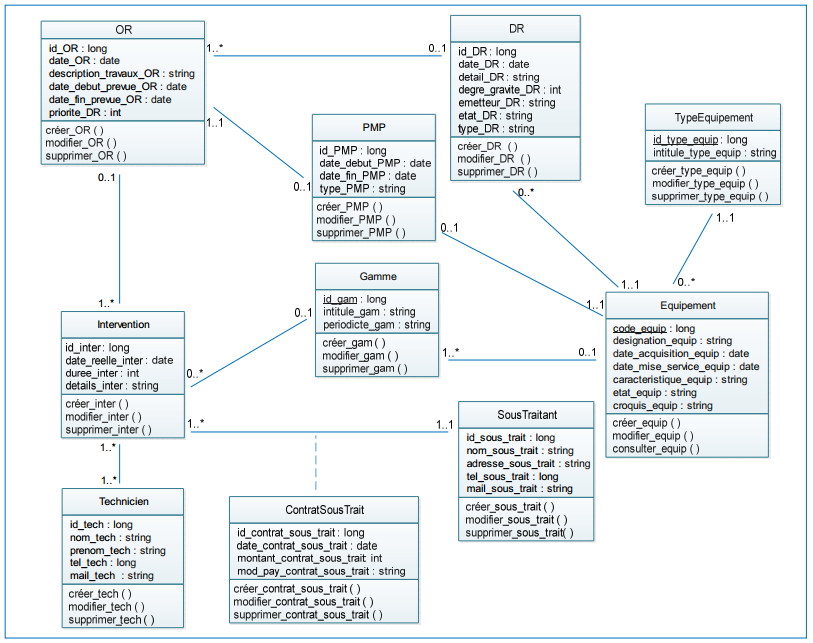
\includegraphics[width=1\linewidth]{./image_chapitre4/Diagramme_classes_maintenance}
	\caption[Diagramme de classe correspondant � la cat�gorie  � Gestion de la maintenance �.]{Diagramme de classe correspondant � la cat�gorie  � Gestion de la maintenance �.}
	\label{fig:Diagramme_classes_maintenance}
\end{figure}
\begin{figure}[H]
	\centering
	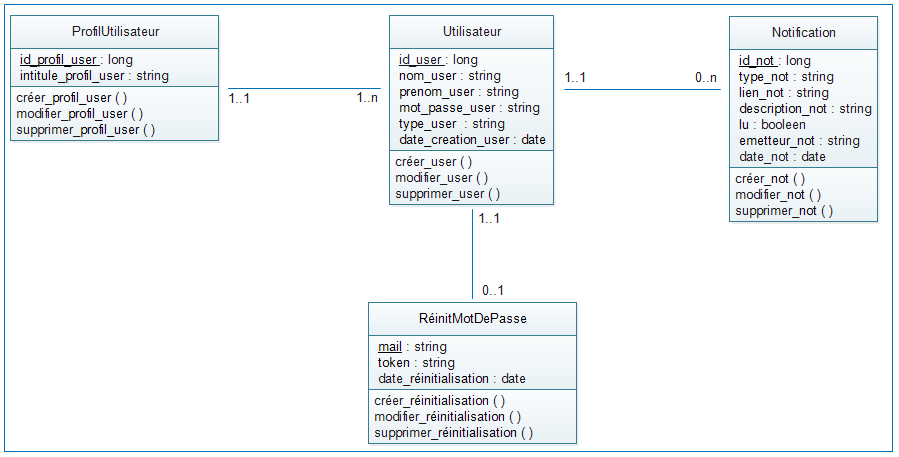
\includegraphics[width=1\linewidth]{./image_chapitre4/Diagramme_classes_admin}
	\caption[Diagramme de classe correspondant � la cat�gorie  � Administration du syst�me �.]{Diagramme de classe correspondant � la cat�gorie  � Administration du syst�me �.}
	\label{fig:Diagramme_classes_admin}
\end{figure}
\newpage
\begin{center}
	\begin{tabular}{|p{3cm}|p{5cm}|p{3cm}|p{2.5cm}|}
		\hline
		\textbf{Classe} &  \textbf{Attribut} &  \textbf{D�signation}&  \textbf{Type} \\
		\hline
		\multirow{14}{*}{Equipement} & code\_equip & code de l'�quipement & entier long   \\ \cline{2-4} 
		& designation\_equip & d�signation de l'�quipement & chaine de crat�res    \\ \cline{2-4} 
		& date\_acquisition\_equip & date d'acquisition de l'�quipement & date    \\ \cline{2-4} 
		& date\_mise\_service\_equip & date de mise en service de l'�quipement & date    \\ \cline{2-4} 
		& caracteristique\_equip & caract�ristique de l'�quipement & chaine de crat�res    \\ \cline{2-4} 
		& etat\_equip & �tat de l'�quipement & chaine de crat�res    \\ \cline{2-4} 
		& croquis\_equip & url du croquis de l'�quipement & chaine de crat�res    \\  
		\hline
		\multirow{4}{*}{TypeEquipement} & id\_type\_equip & identifiant du type de l'�quipement & entier long   \\ \cline{2-4} 
		& intitule\_type\_equip & intitul� du type de l'�quipement & chaine de crat�res    \\   
		\hline
		\multirow{5}{*}{Organe} & code\_org & code de l'organe & entier long   \\ \cline{2-4}  
		& designation\_org & d�signation de l'organe & chaine de crat�res    \\ \cline{2-4} 
		& observation\_org & observation sur l'organe & chaine de crat�res    \\  
		\hline
		\multirow{6}{*}{Gamme} & id\_gam & identifiant de la gamme & entier long   \\ \cline{2-4} 
		& intitule\_gam & intitul� de la gamme & chaine de crat�res    \\ \cline{2-4} 
		& periodicte\_gam & p�riodicit� de la gamme & entier    \\  
		\hline
		\multirow{10}{*}{Operation} & id\_oper & identifiant de l'op�ration & entier long   \\ \cline{2-4} 
		& intitule\_oper & intitul� de l'op�ration & chaine de crat�res    \\ \cline{2-4} 
		& duree\_oper & dur�e de l'op�ration & entier    \\ \cline{2-4}
		& detail\_oper & d�tails de l'op�ration & chaine de crat�res    \\  
		\hline
\end{tabular} \\
\end{center}
\newpage
\begin{center}
		\begin{tabular}{|p{3cm}|p{5cm}|p{3cm}|p{2.5cm}|}
		\hline
		\multirow{10}{*}{Constructeur} & id\_const & identifiant du constructeur & entier long   \\ \cline{2-4} 
		& nom\_const & nom du constructeur & chaine de crat�res    \\ \cline{2-4} 
		& tel\_const & t�l�phone du constructeur & entier long    \\ \cline{2-4}  
		& adresse\_const & adresse du constructeur & chaine de crat�res    \\ \cline{2-4} 
		& email\_const & email du constructeur & chaine de crat�res    \\    
		\hline	
		\multirow{10}{*}{Fournisseur} & id\_four & identifiant du fournisseur & entier long   \\ \cline{2-4} 
		& nom\_four & nom du fournisseur & chaine de crat�res    \\ \cline{2-4} 
		& tel\_four & t�l�phone du fournisseur & entier long    \\ \cline{2-4}  
		& adresse\_four & adresse du fournisseur & chaine de crat�res    \\ \cline{2-4} 
		& email\_four & email du fournisseur & chaine de crat�res    \\    
		\hline
		\multirow{12}{*}{Document} & id\_doc & identifiant du document & entier long   \\ \cline{2-4} 
		& intitule\_doc & intitule du document & chaine de crat�res    \\ \cline{2-4} 
		& type\_doc &  type du document & chaine de crat�res     \\ \cline{2-4} 
		& langue\_doc & langue du document & chaine de crat�res    \\ \cline{2-4} 
		& contenu\_doc & contenu du document & chaine de crat�res     \\ \cline{2-4} 
		& nb\_exemp\_doc & nombre d'exemplaires du document & entier    \\ \cline{2-4} 
		& lieu\_archiv\_doc & lieu d'archivage du document & chaine de crat�res    \\
		\hline
		\multirow{6}{*}{Outillage} & id\_out & identifiant de l'outillage & entier long   \\ \cline{2-4} 
		& designation\_out & d�signation de l'outillage & chaine de crat�res    \\ \cline{2-4} 
		& utilisation\_out & utilisation de l'outillage & chaine de crat�res     \\  
		\hline
\end{tabular} \\
\end{center}
\newpage
\begin{center}
	\begin{tabular}{|p{3cm}|p{5cm}|p{3cm}|p{2.5cm}|}
		\hline
		\multirow{6}{*}{PDR} & id\_PDR & identifiant de la pi�ce de rechange & entier long   \\ \cline{2-4} 
		& intitule\_PDR & intitul� de la PDR & chaine de crat�res    \\ \cline{2-4} 
		& cout\_out & cout de de la PDR & entier     \\  
		\hline
		\multirow{21}{*}{DR} & id\_DR & identifiant de la demande de r�paration & entier long   \\ \cline{2-4} 
		& date\_DR & date de la demande de r�paration & date    \\ \cline{2-4} 
		& detail\_DR & d�tails de la demande de r�paration & chaine de crat�res    \\ \cline{2-4} 
		& degre\_gravite\_DR & degr� de gravit� de la demande de r�paration & entier (0..4)    \\ \cline{2-4} 
		& emetteur\_DR & �metteur de la demande de r�paration & chaine de crat�res    \\ \cline{2-4} 
		& etat\_DR & �tat de la demande de r�paration & chaine de crat�res    \\ \cline{2-4} 
		& type\_DR & type de la demande de r�paration & chaine de crat�res    \\  
		\hline	
		\multirow{15}{*}{OR} & id\_OR & identifiant de l'ordre de r�paration & entier long   \\ \cline{2-4} 
		& date\_OR & date de l'ordre de r�paration & date    \\ \cline{2-4} 
		& description\_travaux\_OR & description des travaux contenus dans l'ordre de r�paration & chaine de crat�res    \\ \cline{2-4}
		& date\_debut\_prevue\_OR & date d�but pr�vue de r�paration & date    \\ \cline{2-4} 
		& date\_fin\_prevue\_OR & date fin pr�vue de r�paration & date    \\ \cline{2-4} 
		& priorite\_OR & priorit� de l'ordre de r�paration & entier (0..4)    \\ 
		\hline	
	\end{tabular} \\
\end{center}
\newpage
\begin{center}
	\begin{tabular}{|p{3cm}|p{5cm}|p{3cm}|p{2.5cm}|}
		\hline
		\multirow{9}{*}{Intervention} & id\_inter & identifiant de l'intervention & entier long   \\ \cline{2-4} 
		& date\_reelle\_inter & date r�elle de l'intervention & date    \\ \cline{2-4} 
		& duree\_inter & dur�e de l'intervention & entier    \\ \cline{2-4} 
		& details\_inter & d�tails des travaux de l'intervention & chaine de crat�res    \\ 
		\hline
		\multirow{10}{*}{Technicien} & id\_tech & identifiant du technicien & entier long   \\ \cline{2-4} 
		& nom\_tech & nom du technicien & chaine de caract�res     \\ \cline{2-4} 
		& prenom\_tech & pr�nom du technicien & chaine de caract�res    \\ \cline{2-4} 
		& tel\_tech & t�l�phone du technicien & entier long    \\ \cline{2-4}
		& mail\_tech & mail du technicien & chaine de crat�res    \\ 
		\hline
		\multirow{12}{*}{PMP} & id\_PMP & identifiant du PMP (Plan de la Maintenance Pr�ventive ) & entier long   \\ \cline{2-4} 
		& date\_debut\_PMP & date d�but du PMP & date     \\ \cline{2-4} 
		& date\_fin\_PMP & date fin du PMP & date     \\ \cline{2-4} 
		& type\_PMP & type de la maintenance pr�ventive (Syst�matique, conditionnelle ou pr�visionnelle) & chaine de caract�res    \\ 
		\hline
		\multirow{10}{*}{SousTraitant} & id\_sous\_trait & identifiant du sous-traitant  & entier long   \\ \cline{2-4} 
		& nom\_sous\_trait & nom du sous-traitant  &  chaine de caract�res   \\ \cline{2-4} 
		& adresse\_sous\_trait & adresse du sous-traitant & chaine de caract�res \\ \cline{2-4} 
		& tel\_sous\_trait & t�l�phone du sous-traitant & entier long     \\ \cline{2-4} 
		& mail\_sous\_trait & mail du sous-traitant & chaine de caract�res     \\ 
		\hline
\end{tabular} \\
\end{center}
\newpage
\begin{center}
	\begin{tabular}{|p{3cm}|p{5cm}|p{3cm}|p{2.5cm}|}
		\hline
		\multirow{11}{*}{ContratSousTrait} & id\_contrat\_sous\_trait & identifiant du contrat de  sous-traitance  & entier long   \\ \cline{2-4} 
		& date\_contrat\_sous\_trait & date du contrat de  sous-traitance  &  date   \\ \cline{2-4} 
		& montant\_contrat\_sous\_trait & montant du contrat de  sous-traitance & entier \\ \cline{2-4} 
		& mod\_pay\_contrat\_sous\_trait & mode de payement du contrat de  sous-traitance & chaine de caract�res      \\ 
		\hline	
		\multirow{8}{*}{Utilisateur} & id\_user & identifiant de l'utilisateur  & entier long   \\ \cline{2-4} 
		& nom\_user & nom de l'utilisateur  &  chaine de caract�res   \\ \cline{2-4} 
		& prenom\_user & pr�nom de l'utilisateur & chaine de caract�res \\ \cline{2-4} 
		& mot\_passe\_user & mot de passe de l'utilisateur & chaine de caract�res \\ \cline{2-4}
		& type\_user & type de l'utilisateur & chaine de caract�res \\ \cline{2-4}
		& date\_creation\_user & date de cr�ation de l'utilisateur  & date   \\ 
		\hline	
		\multirow{7}{*}{ProfilUtilisateur} & id\_profil\_user & identifiant du profil utilisateur  & entier long   \\ \cline{2-4} 
		& intitule\_profil\_user & intitul� du profil utilisateur &  chaine de caract�res   \\ \cline{2-4} 
		& date\_creation\_profil\_user & date de cr�ation du profil utilisateur & date \\
		\hline
		\multirow{4}{*}{Fonctionnalite} & id\_fonc & identifiant de la fonctionnalit� & entier long   \\ \cline{2-4} 
		& intitule\_fonc & intitul� de la fonctionnalit� &  chaine de caract�res   \\ \cline{2-4}
		& url\_fonc & url de la fonctionnalit� &  chaine de caract�res   \\
		\hline
    \end{tabular} \\
    \captionof{table}{Dictionnaire de donn�es du mod�le statique}
    \label{tab39}
\end{center}
\newpage
\subsection{ D�veloppement du mod�le dynamique  }
Le d�veloppement du mod�le dynamique constitue la troisi�me �tape de la partie analyse, elle
consiste � d�gager des sc�narios et � �tudier le comportement des classes du syst�me � partir
des diagrammes de s�quence.\cite{ref08}\\[0.5\baselineskip]
\subsubsection{ Diagrammes de s�quence  }
Le diagramme de s�quence permet de repr�senter les messages �chang�s entre les diff�rents objets du syst�me, avec un ordre chronologique repr�sent� de haut en bas.\cite{ref11}\\[0.5\baselineskip]
 Le diagramme de s�quence n'est pas la seule mod�lisation possible des �changes de messages entre objets ;
le diagramme de communication le permet aussi.\cite{ref08}\\[0.5\baselineskip]
La diff�rence entre les deux diagrammes r�side dans le fait que le diagramme de s�quence
met l'accent sur l'aspect chronologique des communications, alors que le diagramme de communication, quant � lui, met l'accent sur les relations structurelles des participants qui interagissent \cite{ref08}.
Cette diff�rence justifie le choix du diagramme de s�quence dans notre
cas.

Dans ce qui suit, une liste de sc�narios que nous allons repr�senter par des diagrammes de s�quence.

\begin{center}
	\begin{tabular}{|p{15cm}|}
		\hline
		\textbf{Sc�narios des diagrammes de s�quence }  \\
		\hline			
		S'authentifier \\
		\hline
		Ajouter un utilisateur \\
		\hline
		Ajouter un �quipement (sa fiche technique, ses gammes de maintenance, sa nomenclature et sa documentation)\\
		\hline
		Ajouter une demande de r�paration (DR) \\
		\hline
		Ajouter un ordre de travail (OR) \\
		\hline
		G�n�rer le PMP d'un �quipement \\
		\hline
		G�n�rer le planning pr�ventif des �quipements \\
		\hline
		Ajouter un dossier des travaux de sous-traitance \\
		\hline
		G�n�rer les statistiques et les ratios\\
		\hline
	\end{tabular} \\
	\captionof{table}{liste des principaux sc�narios}
	\label{tab34}
\end{center}
\newpage

Dans ce qui suit, nous allons pr�senter chaque sc�nario par un diagramme de s�quence sous UML :\\
\begin{figure}[H]
	\centering
	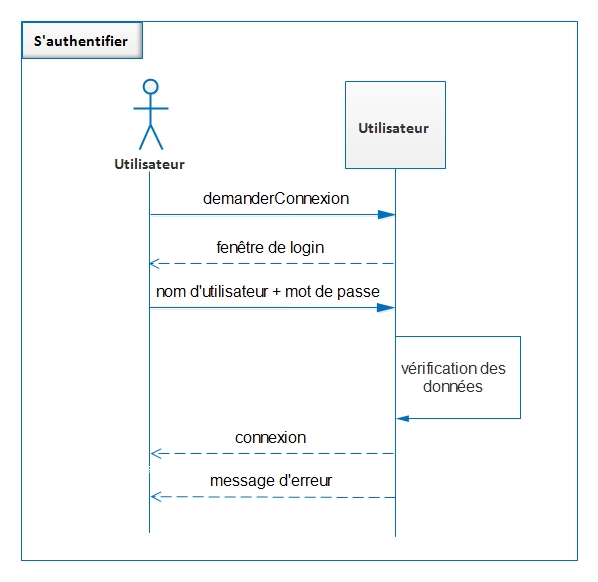
\includegraphics[width=0.9\linewidth]{./image_chapitre4/DSQ_authentification}
	\caption[Diagramme de s�quence de � S'authentifier �.]{Diagramme de s�quence de � S'authentifier �.}
	\label{fig:DSQ_authentifier}
\end{figure}
\newpage

\begin{figure}[H]
	\centering
	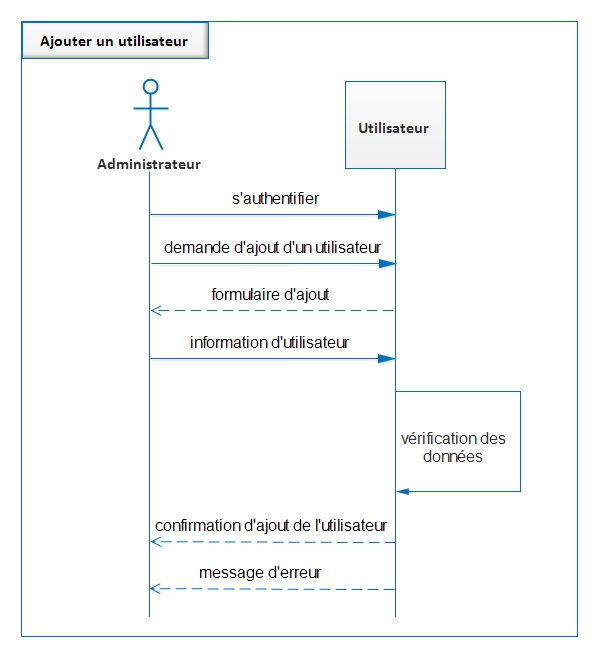
\includegraphics[width=0.9\linewidth]{./image_chapitre4/DSQ_ajouter_user}
	\caption[Diagramme de s�quence de � Ajouter un utilisateur �.]{Diagramme de s�quence de � Ajouter un utilisateur �.}
	\label{fig:DSQ_ajouter_user}
\end{figure}
\newpage

\begin{figure}[H]
	\centering
	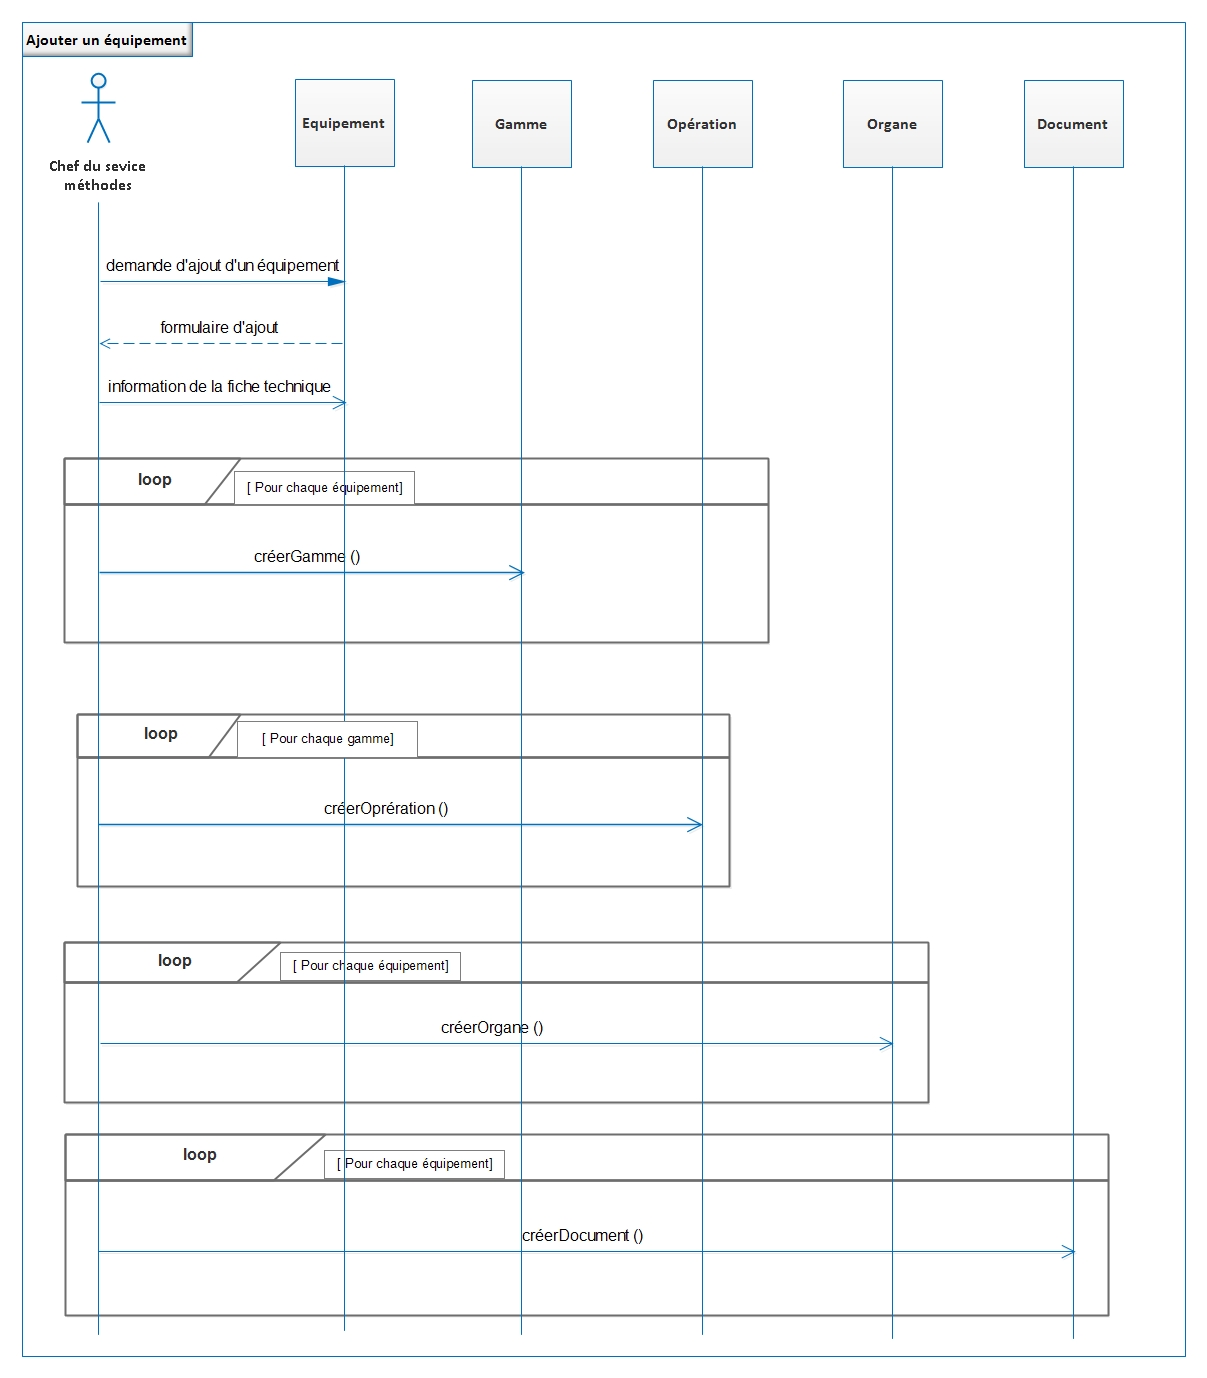
\includegraphics[width=1\linewidth]{./image_chapitre4/DSQ_ajouter_equip}
	\caption[Diagramme de s�quence de � Ajouter un �quipement �.]{Diagramme de s�quence de � Ajouter un �quipement �.}
	\label{fig:DSQ_ajouter_equip}
\end{figure}
\newpage

\begin{figure}[H]
	\centering
	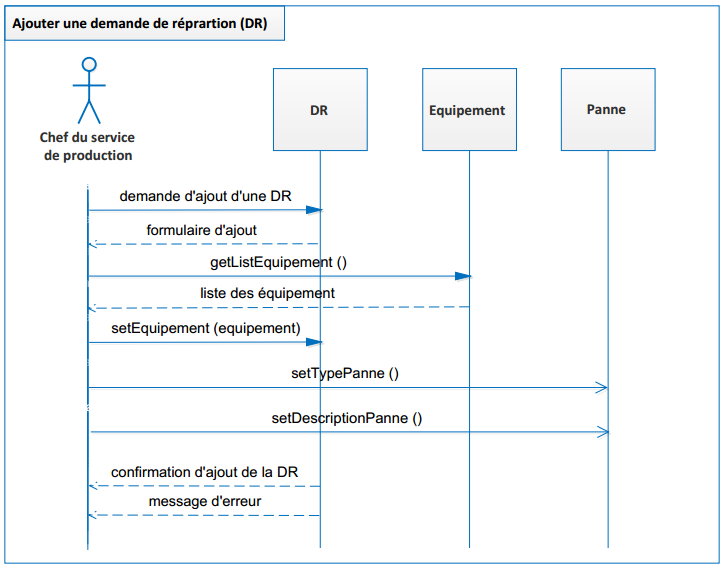
\includegraphics[width=1\linewidth]{./image_chapitre4/DSQ_ajouter_DR}
	\caption[Diagramme de s�quence de � Ajouter une demande de r�paration �.]{Diagramme de s�quence de � Ajouter une demande de r�paration �.}
	\label{fig:DSQ_ajouter_DR}
\end{figure}
\newpage

\begin{figure}[H]
	\centering
	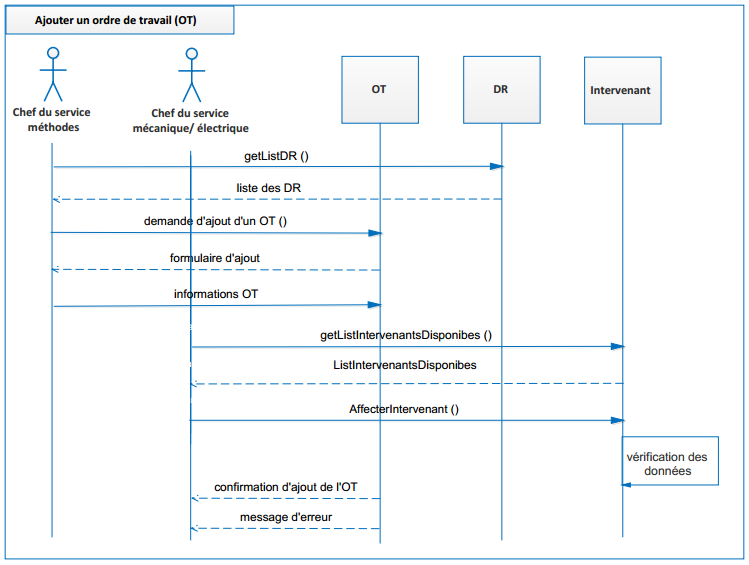
\includegraphics[width=1\linewidth]{./image_chapitre4/DSQ_ajouter_OT}
	\caption[Diagramme de s�quence de � Ajouter un ordre de travail �.]{Diagramme de s�quence de � Ajouter un ordre de travail �.}
	\label{fig:DSQ_ajouter_OT}
\end{figure}
\newpage

\begin{figure}[H]
	\centering
	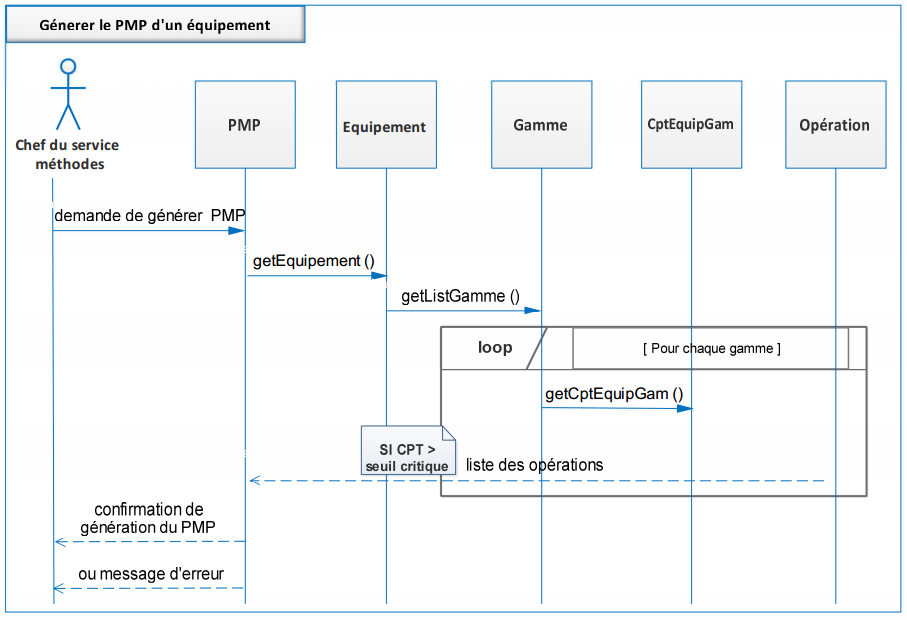
\includegraphics[width=1\linewidth]{./image_chapitre4/DSQ_generer_PMP}
	\caption[Diagramme de s�quence de � G�n�rer le PMP d'un �quipement �.]{Diagramme de s�quence de � G�n�rer le PMP d'un �quipement �.}
	\label{fig:DSQ_generer_PMP}
\end{figure}
\newpage

\begin{figure}[H]
	\centering
	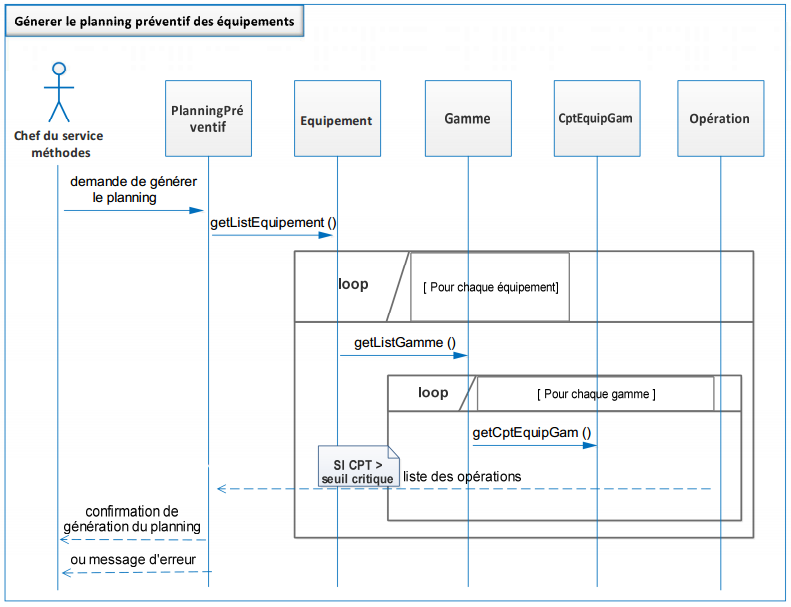
\includegraphics[width=1\linewidth]{./image_chapitre4/DSQ_generer_planning_preventif}
	\caption[Diagramme de s�quence de � G�n�rer le planning pr�ventif des �quipements �.]{Diagramme de s�quence de � G�n�rer le planning pr�ventif des �quipements �.}
	\label{fig:DSQ_generer_planning}
\end{figure}
\newpage

\begin{figure}[H]
	\centering
	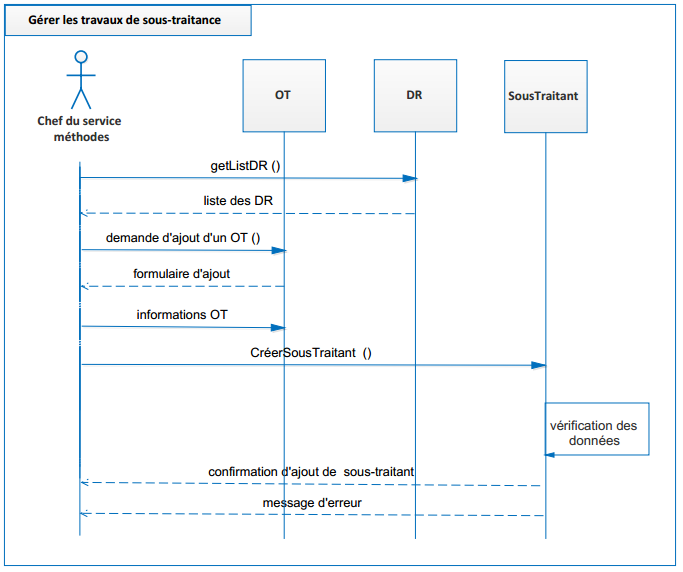
\includegraphics[width=1\linewidth]{./image_chapitre4/DSQ_ajouter_dossier_sous_traitance}
	\caption[Diagramme de s�quence de � Ajouter un dossier des travaux de sous-traitance �.]{Diagramme de s�quence de � 	Ajouter un dossier des travaux de sous-traitance �.}
	\label{fig:DSQ_ajouter_dossierST}
\end{figure}
\newpage



\subsection{ Conclusion  }
� travers ce chapitre nous avons pu mettre en place une solution conceptuelle. D'abord,
nous avons exprim� les besoins fonctionnels et techniques auxquels devra r�pondre notre syst�me en utilisant diagrammes de cas d'utilisation. L'aspect fonctionnel du syst�me attendu nous a permis de bien aborder la phase d'analyse en pr�sentant le d�coupage du syst�me en cat�gories et les diff�rents diagrammes de classes de ces derni�res. Nous avons ensuite d�fini le comportement du syst�me en pr�sentant les diff�rents sc�narios possibles des diagrammes de s�quence. Pour finir, nous avons pr�sent� la base de donn�es qu'utilisera notre application.

\include{pagevide}
\chapter{\sc R�alisation de la solution}
\label{chap:realisation-dep}
Nous  consacrons ce dernier chapitre � la pr�sentation de la phase de r�alisation de notre projet.  La partie r�alisation est tout aussi importante que la conception. En effet,  c'est au cours de celle-ci que nous concr�tisons notre travail. Ceci par l'impl�mentation d'un prototype de la solution pr�sent�e dans les pr�c�dents  chapitres. \\[0.7\baselineskip]
Dans la suite de ce chapitre, nous d�crivons, d'une part, les plates-formes mat�rielles et logicielles sur lesquelles nous avons d�velopp� notre solution, ainsi que les  diff�rents choix techniques que nous avons adopt�. D'autre part, nous pr�sentons notre application, ainsi achev�e, � travers des captures d'�crans des interfaces relatives aux fonctionnalit�s principales.
\section{Environnement de travail}
La r�alisation de tout projet informatique n�cessite des choix mat�riels ainsi que logiciels, lesquels constituent ce que nous appelons environnement de travail.
\subsection{Environnement mat�riel}
Le d�veloppement de l'application s'est fait sur deux machines de type PC portables. Nous donnons ici, la marque et quelques caract�ristiques de chacune d'elles :\\

\begin{itemize}
\item \textbf{Machine 1 :} Acer TravelMate 5735
\begin{itemize}
\item[$\bullet$] Microprocesseur : Intel(R) Core(TM) i5-4210U CPU @ 1.70GHz 2.40 GHz,
\item[$\bullet$] RAM : DDR3 6 GB,
\item[$\bullet$] Disque dur : 1 To.
\end{itemize}
\item \textbf{Machine 2 :} Toshiba  Sattelite L50
\begin{itemize}
\item[$\bullet$] Microprocesseur : Intel(R) Core(TM) i5-4210U CPU @ 1.70GHz 2.40 GHz,
\item[$\bullet$] RAM : DDR3 6 GB,
\item[$\bullet$] Disque dur : 1 To.
\end{itemize}

\end{itemize}

\subsection{Environnement logiciel}
Durant toute la phase de d�veloppement, nous avons utilis� l'environnement logiciel d�crit ci-dessous.
\subsubsection{Syst�me d'exploitation}
Les deux machines utilis�es pour le d�veloppement sont �quip�es d'un syst�me d'exploitation Windows et dont les caract�ristiques sont les suivantes :

\begin{itemize}
	\item \textbf{�dition Windows }: Windows 8.1 Professionnel
	\item \textbf{Type du syst�me :} Syst�me d'exploitation 64 bits
\end{itemize}

\subsubsection{Choix du SGBD}
MySQL est un syst�me de gestion de bases de donn�es relationnelles. Il est distribu� sous une double licence GPL et propri�taire. Il fait partie des logiciels de gestion de base de donn�es les plus utilis�s au monde, autant par le grand public (applications web principalement) que par des professionnels.\\
 \begin{wrapfigure}[4]{r}{3.5cm}
 	
\includegraphics[width=0.8\linewidth]{./image_chapitre5/mysql}
 \end{wrapfigure}
MySQL est un serveur de bases de donn�es d�velopp� dans un souci de performances �lev�es en lecture, ce qui signifie qu'il est davantage orient� vers le service de donn�es d�j� en place que vers celui de mises � jour fr�quentes et fortement s�curis�es. Il est multi-thread et multi-utilisateur.

\subsubsection{Serveur Web}
Tout au long du d�veloppement de notre application, nous avons utilis� le serveur
 \begin{wrapfigure}[4]{r}{3.5cm}
 	
\includegraphics[width=0.8\linewidth]{./image_chapitre5/apache}
 \end{wrapfigure}
 Apache version 2.4.18. Apache HTTP Server (Apache) est un serveur HTTP cr�� et maintenu au sein de la fondation Apache. C'est le serveur HTTP le plus populaire du Web. Il est distribu� selon les termes de la licence Apache. Apache offre diverses fonctionnalit�s dont la possibilit� de d�finir des restrictions d'acc�s gr�ce aux fichiers htaccess ainsi qu'un support de serveurs virtuels.
 
 \section{Choix techniques}
 Avant de se lancer dans le d�veloppement, il est n�cessaire de faire des choix techniques. Ces derniers d�pendent g�n�ralement des objectifs et moyens du projet. Nous ne pouvons pas parler de bons choix dans l'absolu mais des choix bien adapt�s � nos besoins ont �t� adopt�s, et dont la description est donn�e dans la suite de cette section.
 
 \subsection{Choix du langage}
 En d�veloppement, chaque technologie a ses propres sp�cificit�s, ses avantages et ses inconv�nients. Le choix d'une technologie est un choix qui peut �tre qualifi� de crucial, car il engage le d�veloppeur tout au long de son projet. Il existe de nombreuses architectures et langages pour la r�alisation d'application Web. On distingue, g�n�ralement, trois grandes plateformes : 
 \begin{itemize}
 	\item J2EE (Java 2 Platform, Enterprise Edition),
 	\item Microsoft Dot Net,
 	\item et PHP (Hypertext Preprocessor).
 \end{itemize}
 Dans notre cas, nous avons d�cid� d'adopter le langage PHP en tant que principale technologie pour la r�alisation du projet. Notre choix n'est pas fortuit mais d�coule d'une logique que nous pouvons r�sumer en citant les avantages majeurs qu'offre ce langage par rapport aux autres :
 \begin{itemize}
 	\item Tout d'abord, PHP est gratuit et ne n�cessite aucune licence d'utilisation. De plus, il s'agit du langage de programmation Web le plus utilis�,
 	\item C�t� performances, PHP est visiblement plus rapide que les autres langages puisqu'il ne requiert aucune pr�compilation,
 	\item Depuis sa version 5, PHP supporte les concepts de la programmation orient�e objets. Ce qui le change du statut d'un simple langage de script pour pages personnelles et l'ouvre � des r�alisations complexes structur�es et performantes. Ceci a caus� notamment l'apparition de nombreux Frameworks PHP (laravel, Symphony et autres).
 	
 \end{itemize}

\subsection{N�cessit� d'un Framework}
\subsubsection{Framework PHP}
Traduit litt�ralement en fran�ais, le terme Framework signifie �cadre de travail�. C'est un ensemble de biblioth�ques et de conventions permettant le d�veloppement rapide d'une application. Il fournit une palette de briques logicielles et impose suffisamment de rigueur de d�veloppement pour pouvoir produire une application aboutie et facile � maintenir. Ces composants sont organis�s pour �tre utilis�s en interaction les uns avec les autres.

\subsubsection{Avantages des Frameworks}
Certes il n'est gu�re indispensable d'utiliser un Framework pour le d�veloppement d'une application Web. Et contrairement aux id�es re�ues, un Framework, en soi, n'est pas forc�ment un gage de qualit� ni de s�curit�. Tout d�pend de son utilisation et de sa ma�trise, comme tout autre outil. Cependant, les Frameworks de d�veloppement ont de multiples avantages, et parmi lesquels, nous pouvons citer :
\begin{itemize}
	\item D�veloppement rapide d'application (il n'est plus n�cessaire de red�velopper tout un tas de fonctions),
	
	\item Organisation du projet (s�paration des logiques techniques et logiques de pr�sentation),
	
	\item Des composants et biblioth�ques r�utilisables (un composant peut servir dans plusieurs projets),
	
	\item Instauration de bonnes pratiques de codage (comme les standard PSR; PHP Standards Recommendation),
	
	\item La souplesse (laisse de nombreuses libert�s au d�veloppeur).
\end{itemize}

\subsection{Laravel Framework}
Laravel est un framework web open-source �crit en PHP5 respectant le principe 
 \begin{wrapfigure}[4]{r}{4cm}
 	
\includegraphics[width=1\linewidth]{./image_chapitre5/laravel}
 \end{wrapfigure}
 mod�le-vue-contr�leur et enti�rement d�velopp� en programmation orient�e objet
. Laravel est distribu� sous licence MIT.\\
C'est un Framework qui met beaucoup l'accent sur les
bonnes pratiques. Laravel est tr�s utilis� par des grands sites
(vimeo par exemple) et est recommand� pour les
moyens et grands projets.
\subsubsection{Fonctionnalit�s principales}
Zend est consid�r� comme le Framework le plus puissant, gr�ce notamment aux nombreuses fonctionnalit�s qu'il met � la disposition de ses utilisateurs:
\begin{itemize}
	\item \textbf{S�curit� : } protection contre injection SQL, filtrage et validation, etc.
	\item \textbf{Organisation du code :} L'organisation des r�pertoires et des classes suit certaines normes.
	\item \textbf{URL simples et claires :} un syst�me de routage perfectionn� (RESTFul et ressources).
	\item \textbf{Architecture MVC :} offre de base une architecture MVC permettant de s�parer la pr�sentation, la navigation et l'acc�s aux donn�es.
	\item \textbf{Facilitation fonctions courantes  :} acc�s en base de donn�es, authentification, droits d'acc�s, pagination etc.
\end{itemize}

\subsubsection{Choix de Laravel}
Nous avons pr�f�r� Laravel aux autres Frameworks PHP car c'est un Framework qui nous est familier, et dont les m�canismes de fonctionnement ne nous sont pas totalement m�connus. Ceci diminue consid�rablement le temps d'apprentissage et am�liore la capacit�  � r�soudre les probl�mes li�s au d�veloppement durant la phase de codage.\\[0.7\baselineskip]
Par ailleurs notre choix est aussi motiv� par les nombreux avantages offerts par ce Framework :
\begin{itemize}
	\item Il est soutenu par une large communaut� et b�n�ficie d'une grande notori�t�, 
	
	\item Une courbe d'apprentissage relativement rapide (contrairement aux autres grands framework),
	
	\item Des librairies sous forme de module,
	
	\item Librairie stable et fiable.
	
\end{itemize}

\subsection{Eloquent ORM}
\subsubsection{D�finition d'un ORM}
Un ORM, pour Object-Relational Mapping, est une couche d'abstraction entre l'application et la base de donn�es. Il donne l'illusion de travailler avec une base de donn�es orient�e objet. En effet, il permet de mapper directement la base de donn�es relationnelle en objet.  De ce fait, le d�veloppeur ne se soucie quasiment plus des requ�tes SQL ni du SGBD que l'application utilise.
\subsubsection{Eloquent}
Eloquent ORM inclus avec Laravel permet de travailler facilement avec la base de donn�es.
Chaque table de base de donn�es dispose d'un "mod�le" correspondant qui est utilis� pour
interagir avec cette table. Les mod�les permettent d'effectuer toute les op�rations sur une table (insertion, modification , suppression) et offre une multitudes de fonctions qui permettent d'interagir avec les donn�es sans avoir recours a des requ�tes SQL complexes.

\subsection{Choix du standard de d�veloppement}
\label{sec:standard-dev} 
Il est g�n�ralement int�ressant de suivre un certain design pattern (patron de conception) pour rendre le code plus ais� � maintenir et � faire �voluer. \\[0.7\baselineskip]
Pour le d�veloppement de notre application, nous avons d�cid� de suivre le pattern MVC. L'architecture MVC est devenue un standard de conception des applications Web modernes. Suivant ce mod�le,  la plupart du code d'une application se retrouve dans l'une de ces couches : pr�sentation, logique m�tier, et acc�s aux donn�es. Le pattern MVC mod�lise cette s�paration d'une mani�re quasi-parfaite. Cette s�paration est indispensable pour maintenir le code global organis�, particuli�rement lorsque plusieurs d�veloppeurs travaillent ensemble sur la m�me application.\\[0.7\baselineskip]
MVC est tr�s utilis� avec PHP. Il est m�me devenu le pattern architectural le plus utilis� dans les Frameworks PHP, et Laravel n'en fait pas exception.\\[0.7\baselineskip]
La figure suivante r�sume les diff�rentes interactions entre les couches du mod�le MVC.   
\begin{figure}[h!]
	\centering
	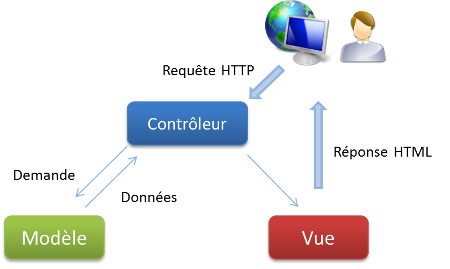
\includegraphics[width=0.7\linewidth]{./image_chapitre5/mvc}
	\caption{Sch�ma des interations entre couches du mod�le MVC}
\end{figure}

\subsubsection{Organisation du projet}
La hi�rarchie de notre projet est comme pr�sent�e dans la figure ci-dessous. Chaque module poss�de ses propre contr�leurs, vues et repositories (classes de gestion de donn�es).
La s�paration en module permet de simplifier la t�che de maintenance du code et l'am�lioration du projet.
\begin{figure}[h!]
	\centering
	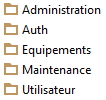
\includegraphics[scale=1.3]{./image_chapitre5/application}
	\caption{Arborescence de l'application selon le pattern MVC}
	\label{fig:folder-structure}
\end{figure}\\[0.7\baselineskip]
Dans ce qui suit, nous donnons une br�ve explication de chaque r�pertoire du projet : 

\begin{itemize}
	\item \textbf{Module Administration :} qui contient les contr�leurs et vues relatifs l'administration de l'application.
	\item \textbf{Module Auth :} ce module fourni permet la gestion d'authentification des utilisateurs (gestion des sessions).
	\item \textbf{Module Equipements :} qui contient les contr�leurs et vues n�cessaires � la fonctionnalit� d'inventaire des �quipements (nomenclature, gammes, documentation, fournisseurs ...) .
	\item \textbf{Module Maintenance :} contient les contr�leurs et vue pour la gestion de la maintenance (corrective et pr�ventive).
	\item \textbf{Utilisateur :} qui contient les contr�leurs et vues n�cessaires qui permet la gestion des notifications (en temps r�el).
	
\end{itemize}

\subsection{La s�curit� de l'application}
La s�curit� des syst�mes d'information est l'ensemble des mesures techniques et
de protection permettant � un syst�me d'information de r�sister � des �v�nements susceptibles
de compromettre la disponibilit�, l'int�grit� ou la confidentialit� des donn�es stock�es.
Etant une solution web, notre solution est expos�e d'avantages aux risques de failles
s�curitaires. Par cons�quent nous nous somme int�resser en premier lieu aux attaques les plus
courantes, pour enfin trouver des solutions et prot�ger au mieux notre application.

\subsubsection{S�curisation des interactions avec l'utilisateur}
\label{sec:secu-inject} 
Les applications Web sont caract�ris�es par un tr�s grand nombre d'�changes entre l'utilisateur et le serveur. Ces �changes constituent une v�ritable source de risques qu'il faut ma�triser.

\subsubsection*{Validation et filtrage des formulaires}
Laravel fournit deux composants facilitant la validation des formulaires : FormRequest. Une erreur de validation sera g�n�r�e quand le type de donn�es re�ues d'un ou plusieurs champs ne correspondent � ce que l'on attend r�ellement. De plus, une validation cot� client (javascript) est effectu� en premier lieu pour all�ger la charge du serveur. 

\subsubsection*{Protection contre les injections SQL}
C'est une des plus vieilles failles connues mais c'est �galement la plus dangereuse. Une injection SQL consiste � saisir des requ�tes SQL dans un champ de formulaire, pour obtenir des informations sur le fonctionnement de l'application et de passer outre certaines autorisations.
La protection contre les injections SQL est assur�e par Eloquent ORM. L'utilisation des m�thodes fourni par ce dernier permet d'�viter ce genre d'attaque.

\subsubsection*{Protection contre les attaques CSRF}
Cette attaque est relativement simple � mettre en place et consiste � envoyer � un client authentifi� sur un site un script dissimul� (dans une page web ou un email) pour lui faire accomplir une action � son insu.
Pour se pr�munir contre ce genre d'attaque Laravel g�n�re un token al�atoire associ� au formulaire de telle sorte qu'� la soumission ce token est v�rifi� pour �tre s�r de l'origine (avec le composant VerifyCsrfToken).

\subsubsection*{Protection contre les attaques XSS}
C'est une technique qui consiste � injecter du code HTML contenant du JavaScript dans une page pour le faire ex�cuter � un utilisateur (pour voler une session ou un mot de passe par exemple).
Les vuln�rabilit�s de type XSS apparaissent dans les vues. Pour pallier ce probl�me, Laravel propose le composant Blade. Ce dernier propose une syntaxe (double accolades \{\{\ \}\}) qui permet d'�chapper le code html et ainsi afficher les balise <> plut�t que de les ex�cuter.


\subsubsection{Authentification et contr�les d'acc�s } 
Un �l�ment clef de la s�curisation d'une application web consiste � d�terminer si un utilisateur donn� a le droit d'acc�der � la ressource qu'il demande. Cette s�curisation s'effectue en deux �tapes : une �tape d'authentification et une �tape d'autorisation permettant de v�rifier que l'utilisateur a bien le droit d'acc�der � la ressource souhait�e.
La plupart des Frameworks PHP modernes poss�dent les concepts d'authentification ou de contr�le d'acc�s. Dans le cas de Laravel, l'authentification est g�r�e par le composant
\begin{BVerbatim}
Controller\auth
\end{BVerbatim}, alors que le contr�le d'acc�s est g�r� par 
\begin{BVerbatim}
Middelware\authenticate
\end{BVerbatim}

\subsection{Autres choix technologiques}
\subsubsection{jQuery}
\begin{wrapfigure}{r}{4cm}
	
\includegraphics[width=4cm,height=2cm]{./image_chapitre5/jquery}
\end{wrapfigure}
jQuery est une biblioth�que libre d�velopp�e en JavaScript (dit �galement Framework JavaScript). C'est un logiciel open source distribu� sous les licences combin�es du MIT et GPL.  JQuery permet de manipuler d'une mani�re ais�e le Document Object Model plus connu sous son abr�viation DOM, et qui est un standard du W3C. \\[0.7\baselineskip]
En plus de l'utilisation de cette librairie, plusieurs plugins ont �t� utilis�s, les plus importants sont:
\begin{itemize}
	\item Bootstrap validation.
	\item Datatables.js.
	\item Moment.js.
	\item notifications.js
	\item fullcalendar.js.
	\item waitme.js.
\end{itemize}
\subsubsection{Node.js}
\begin{wrapfigure}{r}{4cm}
	
\includegraphics[width=4cm,height=2cm]{./image_chapitre5/nodejs}
\end{wrapfigure}
Node.js est une plateforme logicielle libre et �v�nementielle en JavaScript orient�e vers les applications r�seau qui doivent pouvoir monter en charge. il est distribu� sous licence MIT. Concr�tement, node.js est un environnement d'assez bas niveau permettant d'ex�cuter du javascript non plus dans le navigateur web mais sur le serveur.
\subsubsection{Socket.IO}
socket.io est l'une des biblioth�ques les plus plus utilis�es avec Node.js. Elle permet de
\begin{wrapfigure}{r}{4cm}
	
\includegraphics[width=4cm,height=2cm]{./image_chapitre5/socketio}
\end{wrapfigure}
faire tr�s simplement de la communication synchrone dans l'application, c'est-�-dire de la communication en temps r�el.socket.io se base sur plusieurs techniques diff�rentes qui permettent la communication en temps r�el, La plus connue d'entre elles est WebSocket (API javascript).\\[0.5\baselineskip]
 
 Ces deux technologies ( Node.JS et Socket.IO) combin�es aux composant app\textbackslash Events de Laravel nous ont permet de mettre en place un syst�me de notification en temps r�el.
 
 \section{Interfaces de l'application}
 Nous donnons dans ce qui suit les principales interfaces de l'application produite.
 \subsection{Interface d'authentification}
 
 \subsubsection*{Authentification}
 
 C'est la premi�re interface qui apparait au lancement de l'application (voir figure \autoref{fig:interface-auth}).
 \begin{figure}[H]
 	\centering
 	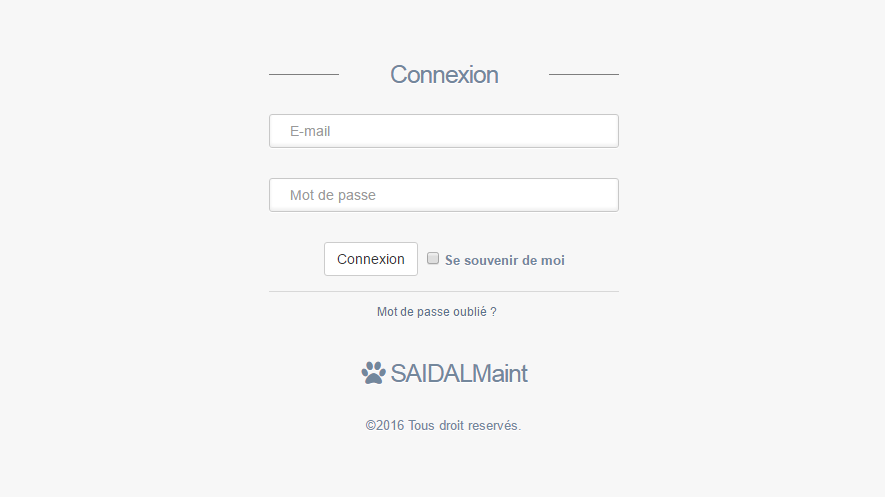
\includegraphics[width=1\linewidth]{./image_chapitre5/connexion}
 	\caption{Interface d'authentification de l'application}
 	\label{fig:interface-auth}
 \end{figure}
 
 \subsubsection*{R�initialisation de mot de passe}
 En cas d'oubli de mot de passe, l'utilisateur peut demander un nouveau mot de passe que le syst�me envoie par e-mail. �videmment l'utilisateur doit introduire une adresse e-mail valide (c'est-�-dire qui existe dans la base de donn�es).
 \begin{figure}[h!]
 	\centering
 	\includegraphics[width=1\linewidth]{./image_chapitre5/reset}
 	\caption{R�initialisation de mot de passe en cas d'oubli}
 \end{figure}
 
 \section{Conclusion}
 � travers ce dernier chapitre, nous avons d�crit la partie r�alisation de notre solution. Ainsi, nous avons expos�, en premier lieu, l'environnement mat�riel et logiciel dans lequel nous avons d�velopp� notre application, suivi d'une pr�sentation de nos diff�rents choix technologique.\\[0.7\baselineskip]
 Nous avons, par la suite, pr�sent� les interfaces les plus significatives de notre application moyennant des captures d'�crans, tout en donnant des explications br�ves des fonctionnalit�s offertes par l'application finale.
\include{pagevide}

%-----------------------Conclusion-----------------------%
\fancyhead[LE,RO]{} \fancyhead[LO]{}\fancyhead[RE]{}
\fancyhead[C]{\bfseries Conclusion g�n�rale}
\renewcommand{\footrulewidth}{0.5pt}
\phantomsection
\addcontentsline{toc}{chapter}{\numberline{}Conclusion g�n�rale}
\chapter*{Conclusion g�n�rale et perspectives}

Dans ce m�moire nous avons pr�sent� le travail r�alis� dans le cadre de notre projet de fin
d'�tudes, et dont l'objectif �tait la conception et la r�alisation d'un syst�me d'information pour la gestion de la maintenance au sein du groupe SAIDAL. Cette derni�re �prouve des besoins dans la gestion actuelle de la maintenance. Cette derni�re, �tant une gestion manuelle, ne permet pas d'effectuer des intervention en temps voulu, ne permet pas une bonne planification des interventions pr�ventive et encore moins une bonne tra�abilit� de l'information. L'entreprise � jug� utile de doter son service de maintenance d'une application de gestion de la maintenance assist� par ordinateur.\\[0.5\baselineskip]
Une premi�re �tape �tait d'effecteur une �tude bibliographique sur la maintenance afin de d�couvrir ce domaine. Nous avons pris connaissance des concepts cl� de la maintenance, � savoir , les diff�rents type de maintenance existants (corrective, pr�ventive), les gammes de maintenance, le PMP, ainsi que les objectifs de la fonction maintenance. Cette �tude nous a aussi permet d'appr�hender les concepts de la GMAO et les fonctionnalit�s qu'elle offre et son apport dans le domaine de la maintenance.\\[0.5\baselineskip]
La deuxi�me �tape d'effectuer une �tude de l'existant. �a a permet de se familiariser avec les diff�rents proc�dures de maintenance au sein de SAIDAL, et ainsi de d�tecter les points faibles de la gestion actuelle et ainsi proposer une solution optimal et propre leurs processus de maintenance.\\[0.5\baselineskip]
La troisi�me �tape porte sur la conception, nous 

Les principaux objectifs de ce projets sont atteints, n�anmoins un travail parfait n'existe jamais et notre travail n'en fait pas exception. Des perspectives d'am�lioration peuvent �tre envisag�es:
\begin{itemize}

\item Int�grer le syst�me de gestion des stocks dans la GMAO (stock de pi�ces de rechange).
\item Int�grer le syst�me de gestion des immobilisations dans la GMAO.
\item D�ployer le syst�me sur les autre sites de production (ce qui va amener � apporter des modifications majeurs vu que le processus de maintenance est diff�rent d'un site � un autre).
\item Int�grer la gestion �lectronique des documents (GED).
\item Concevoir un syst�me d'aide � la d�cision bas� sur les donn�es issues de notre syst�me.
\item int�grer une fonctionnalit� de gestion des contrat de sous-traitance.  
\end{itemize}  



%----------------------Bibliographie---------------------%
\fancyhead[LE,RO]{} \fancyhead[LO]{}\fancyhead[RE]{}
\fancyhead[C]{\bfseries Bibliographie - Webographie}
\renewcommand{\footrulewidth}{0.5pt}
\phantomsection
\renewcommand\bibname{Bibliographie - Webographie}
\addcontentsline{toc}{chapter}{\numberline{}Bibliographie - Webographie}
\begin{thebibliography}{MON00}
\expandafter\ifx\csname fonteauteurs\endcsname\relax
\def\fonteauteurs{\scshape}\fi

\bibitem[\bfseries AFN02]{ref02}
\bgroup\fonteauteurs\bgroup AFNOR\egroup\egroup{} :
\newblock Maintenance industrielle: Fonction maintenance. indice de classement:
  Fd x 60-000.
\newblock Disponible en ligne sur:
  \url{http://imis.angers.free.fr/site/IMG/pdf/FDX_60-000.pdf}, Mai 2002.
\newblock [Consult� le 20 Octobre 2015].

\bibitem[\bfseries BUC00]{web02}
Nicolas \bgroup\fonteauteurs\bgroup BUCHY\egroup\egroup{} :
\newblock La gestion de la maintenance assist�e par ordinateur et la
  maintenance des logiciels.
\newblock Disponible en ligne sur:
  \url{http://s3.amazonaws.com/publicationslist.org/data/gelog/ref-507/115.pdf},
  2000.

\bibitem[\bfseries dl11]{web09}
Minist�re de~\bgroup\fonteauteurs\bgroup l'Industrie\egroup\egroup{} :
\newblock Rapport sectoriel n�01: L'industrie pharmaceutique.
\newblock page~3, Janvier 2011.

\bibitem[\bfseries DRE08]{web03}
Vincent \bgroup\fonteauteurs\bgroup DRECQ\egroup\egroup{} :
\newblock La gmao en quelques lignes.
\newblock Disponible en ligne sur:
  \url{http://www.conseilorga.com/Documents/octobre%202008%20-%20La%20GMAO%20en%20quelques%20lignes.pdf},
  Octobre 2008.
\newblock [Consult� le 20 Octobre 2015].

\bibitem[\bfseries AA13]{web07}
Ouardia \bgroup\fonteauteurs\bgroup ATEK\egroup\egroup{} et Farida
\bgroup\fonteauteurs\bgroup ADMANE\egroup\egroup{} :
\newblock Introduction aux syst�mes d'information.
\newblock Cours de syst�me d'information (2CPI), Ecole nationale superieure
d'informatique, ALGER, 2013.

\bibitem[\bfseries KAF01]{ref04}
H�di \bgroup\fonteauteurs\bgroup KAFFEL\egroup\egroup{} :
\newblock {\em Contribution La maintenance distribu�: concepts, �valuation et
  mise en \oe uvre}.
\newblock Th\`ese de doctorat, universit� laval qu�bec, Octobre 2001.

\bibitem[\bfseries LAC11]{web08}
Mohamed-Ch�rif \bgroup\fonteauteurs\bgroup LACHICHI\egroup\egroup{} :
\newblock Lotfi benbahmed, pr{\'e}esident du conseil national de l'ordre des
  pharmaciens, au forum de "libert{\'e}".
\newblock {\em "LIBERT{\'E}"}, page~6, 16 mars 2011.

\bibitem[\bfseries MEC04]{ref06}
Bernard \bgroup\fonteauteurs\bgroup MECHIN\egroup\egroup{} :
\newblock {\em Documentation de la fonction maintenance}.
\newblock Ed. Techniques Ing�nieur, 2004.

\bibitem[\bfseries MON00]{ref01}
Fran�ois \bgroup\fonteauteurs\bgroup MONCHY\egroup\egroup{} :
\newblock {\em Maintenance: M�thodes et organisations}.
\newblock Dunod \'edition, 2000.

\bibitem[\bfseries Oph08]{ref05}
D.~\bgroup\fonteauteurs\bgroup Ophelie\egroup\egroup{} :
\newblock Gestion de la maintenance assist�e par ordinateur.
\newblock {\em Publications Oboulo. com}, 2008.

\bibitem[\bfseries RUF11]{web04}
Jean-Michel \bgroup\fonteauteurs\bgroup RUFFIN\egroup\egroup{} :
\newblock pourquoi une gmao.
\newblock Disponible en ligne sur:
  \url{www.jmr-gmao.com/FTPJMR/Pourquoi%20une%20GMAO.doc}, 2011.
\newblock [Consult� le 20 Octobre 2015].

\bibitem[\bfseries SML97]{ref03}
Marc \bgroup\fonteauteurs\bgroup SAINT-MARSEILLE\egroup\egroup{} et Jean-Bruno
  \bgroup\fonteauteurs\bgroup LAPOINTE\egroup\egroup{} :
\newblock {\em La gestion des �quipements: vers l'entretien pr�ventif}.
\newblock Association paritaire pour la sant� et la s�curit� du travail
  secteur fabrication de produits en m�tal et de produits �lectriques
  \'edition, 1997.

\bibitem[\bfseries weba]{web05}
Comparatif des logiciels gmao.
\newblock Disponible en ligne sur:
  \url{http://gii.polytech.up.univ-mrs.fr/deuterium/page_guide.php?num_page=66}.
\newblock [Consult� le 20 Octobre 2015].

\bibitem[\bfseries webb]{web06}
Gestion de la maintenance: les logiciels de gmao.
\newblock Disponible en ligne sur:
  \url{www.mesures.com/pdf/old/778GA_logiciel_GMAO.pdf}.
\newblock [Consult� le 20 Octobre 2015].

\bibitem[\bfseries webc]{web10}
Site officiel du groupe saidal.
\newblock Disponible en ligne sur: \url{https://www.saidalgroup.dz}.
\newblock [En ligne: Consult� le 20 Octobre 2015].

\bibitem[\bfseries web14]{web01}
Introduction � la maintenance.
\newblock Disponible en ligne sur:
  \url{http://www.technologuepro.com/maintenance-industrielle/chapitre-4-la-documentation-enmaintenance.pdf},
  2014.
\newblock [Consult� le 20 Octobre 2015].

\bibitem[\bfseries ROQUES VAL, 2004]{ref07}
Pascal \bgroup\fonteauteurs\bgroup ROQUES\egroup\egroup{} and
Franck  \bgroup\fonteauteurs\bgroup VALLEE\egroup\egroup{} :
\newblock {\em UML 2 en action de l'analyse des besoins � la conception J2EE}.
\newblock 3�me �dition Ed. EYROLLES, 2004.

\bibitem[\bfseries ROQUES VAL, 2007]{ref08}
Pascal \bgroup\fonteauteurs\bgroup ROQUES\egroup\egroup{} and
Franck  \bgroup\fonteauteurs\bgroup VALLEE\egroup\egroup{} :
\newblock {\em UML 2 en action de l'analyse des besoins � la conception J2EE}.
\newblock 4�me �dition Ed. EYROLLES, 2007.

\bibitem[\bfseries ROQUES, 2008]{ref09}
Pascal \bgroup\fonteauteurs\bgroup ROQUES\egroup\egroup{} :
\newblock {\em UML 2 Mod�liser une application web }.
\newblock 4�me �dition Ed. EYROLLES, 2008.

\bibitem[\bfseries MB11]{web11}
Mohammed Amine   \bgroup\fonteauteurs\bgroup MOSTEFAI\egroup\egroup{} et Sofiane  
\bgroup\fonteauteurs\bgroup BATATA\egroup\egroup{} :
\newblock Expression des besoins.
\newblock Cours d'IGL (Introduction de G�nie Logiciel) (1CS), Ecole nationale superieure
d'informatique, ALGER, 2011.

\bibitem[\bfseries webd]{web12}
Choix d'une architecture trois-tiers
\newblock Disponible en ligne sur:
\url{http://cedric.babault.free.fr/rapport/node4.html}.
\newblock [Consult� le 26 Avril 2016].



\bibitem[\bfseries AUDIBERT, 2009]{ref11}
Laurent \bgroup\fonteauteurs\bgroup AUDIBERT\egroup\egroup{} :
\newblock {\em UML 2 De L?apprentissage � La Pratique }.
\url{http://laurent-audibert.developpez.com/Cours-UML/?page=introduction-modelisation-objet#L1-4-3-f},
2009.
\newblock [Consult� le 17 Mai 2016].



\end{thebibliography}

%----------------------Webographie---------------------%
%\fancyhead[LE,RO]{} \fancyhead[LO]{}\fancyhead[RE]{}
%\fancyhead[C]{\bfseries Bibliographie - Webographie}
%\renewcommand{\footrulewidth}{0.5pt}
%\phantomsection
%\renewcommand\bibname{Webographie}
%\addcontentsline{toc}{chapter}{\numberline{} Webographie}
%\begin{thebibliography}{site5}

\bibitem[Doctissimo, 2015]{site5}
Doctissimo (2015).
\newblock
\url{http://www.doctissimo.fr/html/dossiers/meningite/sa_5040_meninge.htm}.
\newblock [En ligne; Consult{\'e} le 29-Novembre-2015].

\end{thebibliography}
%--------------------------Page vide---------------------%
\include{pagevide}\fancyhf{}
\renewcommand{\headrulewidth}{0pt}%
\renewcommand{\footrulewidth}{0pt}

\end{document}
